% vim: nospell
% mainfile: master.tex
\input set/preamble.tex
\input set/macros.tex
\input set/listings.tex

\begin{document}

% Front matter %%%%%%%%%%%%%%%%%%%%%%%%%%%%%%%%%%%%%%%%%%%%%%%%%%%%%%%%%%%%%%%%%
\pagenumbering{roman}
\pagestyle{empty}
\input set/frontpage
\input set/titlepage
\pagestyle{fancy}
\setcounter{page}{1}
\tableofcontents
\cleardoublepage

% Main matter %%%%%%%%%%%%%%%%%%%%%%%%%%%%%%%%%%%%%%%%%%%%%%%%%%%%%%%%%%%%%%%%%%
\setcounter{page}{1}
\pagenumbering{arabic}

% Intro
\chapter{Introduction}
\label{cha:intro}

%% Motivation
The mobile phone era began to take its modern form in the eighties when the development of analog cell-based mobile phone systems began. The AMPS systems, developed by Bell Labs and installed in the United States in 1982, being the most successful of the first generation mobile phone systems, proved that mobile personal telephony was here to stay \cite{tanenbaum2012computer}. In the second generation, speech was transmitted in digital form instead of analog. The GSM system from Europe became the de-facto world wide standard for 2G, while still only being aimed at voice communication \cite{tanenbaum2012computer}. Towards the third generation, and with the transition towards smartphones, mobile phones were no longer only a means of communicating voice and short messages, but also a means of accessing the Internet and exchanging data. The increase in music and video services online made the demand for higher data rates larger and larger while the number of users increased as well.

% LTE: MIMO antennas for higher performance: Requires low correlation + high efficiency
The technology for the fourth generation is the Long Term Evolution (LTE). The fourth generation of mobile phone systems aimed to increase the data rates as well as getting a more seamless interaction with wired and wireless IP networks \cite{tanenbaum2012computer}. A way of getting there is the use of MIMO, i.e.\ having multiple antennas in the mobile phones, making it possible to either communicate data in parallel, increasing the data rate, or to increase the signal strength using diversity techniques. For this reason, the LTE specification supports multiple antennas to be integrated for LTE MIMO and diversity use \cite{holma2011lte}.

In order to achieve good MIMO and diversity performance, the correlation between the radiation patterns of the LTE antennas should be low, i.e.\ the signals received by the two should be as different as possible in order to gain the most \cite{Tim2012Practical}. Patterns can be de-correlated by spacing the antennas far apart compared to the wavelength. However, this is not practical in a mobile phone at the low-band frequencies as the free-space wavelength at \SI{700}{MHz} is \SI{429}{mm}. The correlation can be improved by having the antennas polarized differently but this is no easy task.

% Lower frequency bands may be deployed (cite: Samantha2015tunableAntennas)
The demand for bandwidth increases as more and more users desire a greater throughput, new bands are being licensed. Part of the spectrum around \SI{600}{MHz}, previously used for television broadcasting, is being considered for extending the LTE bands \cite{Samantha2015tunableAntennas}. While the lower frequencies provide great penetration for long-range communication, the wavelength, and hence the antennas, tend to either increase in size or decrease the efficiency or bandwidth \cite{hilbert2015tradeoff}. 

% Screen-dominant: Antennas near edge
% Less space in phones -> smaller -> less BW/higher Q (cite: hilbert2015tradeoff)
In modern mobile phones, the screen is the dominant user interface, taking up almost all of the front-side of the phone. This means that only little space, along the edge of the phone, is available for antennas. As described in \cite{hilbert2015tradeoff}, the smaller available area means that either the efficiency or the bandwidth must decrease.

% Phones in-use: Detuning cite: pelosi2009grip
As the antennas are placed close to the edge of the phone, they are in very close proximity to the user. This has the effect of absorbing part of the power and also detuning the antenna \cite{pelosi2009grip}. The antennas can be designed to have resonances which are determined by a matching circuit placed immediately before the antenna but as the antenna changes its resonance based on whether or not a user is present, the matching circuitry would need to be variable to account for different use cases.

% Solution: Lower BW, Tunable matching network
The solution to the low available bandwidth and the detuning caused by the user, is to use a digitally controllable tuner in the matching network. This makes it possible to have a lower bandwidth, covering a minimum of only the largest LTE band -- not all at the same time -- and then re-tune the resonance to the desired band. This way, all bands could be covered at a decent efficiency and the loading caused by the user could be minimized by counter-tuning the antenna based on the user's behavior.

Several solutions exist for digitally tunable capacitors. Varactor diodes can be used as tunable capacitors by altering the bias voltage while CMOS tunable capacitors consist of banks of capacitors which are switched in and out of circuit using CMOS technology. MEMS tunable capacitors come in two variants where one uses MEMS switches to switch capacitors like the CMOS tuners. The other variant alters the proximity of two parallel plates, thereby changing the capacity \cite{gu2014rf}.

% State-of-the-art
Previous antenna designers have dealt with developing tunable antennas for the LTE bands supporting MIMO. Using MEMS tunable capacitors, \cite{ilvonen2014multiband} managed to design a quite efficient design with two antennas. The ground clearance for this design is \SI{15}{mm} and may be closing in on the size constraints for practical implementation in a phone. In \cite{morris2014tunable}, a single antenna was designed using a MEMS tuner. While being small and rather efficient, this design only consisted of a single antenna and does, for this reason, not support MIMO for LTE. In \cite{xia2015compact}, a CMOS tuner was used and a very compact and efficient design has been developed while still only for a single antenna. A MEMS tuner was used for tuning the side antenna in \cite{tatomirescu2015alternative} while the top antenna was fixed and showed good results. This design, however, did only cover the low bands below \SI{960}{MHz}. Finally, in \cite{trinh2016reconfigurable}, a design for reaching towards 5G was designed. Showing very good results, the design only consisted of a single antenna.

In this project, a dual resonance antenna design for LTE supporting MIMO will be designed. The goal is to minimize the ground clearance so the antenna would be attractive in a practical design. The aim is to investigate how ground clearance affects the bandwidth and design a MIMO antennas system using the smallest practical clearance, covering all LTE bands from \SI{700}{MHz} to \SI{960}{MHz} and from \SI{1710}{MHz} to \SI{2650}{MHz}.

%% Overview
% Report overview
The first part of the report -- Chapter~\ref{cha:problem_analysis} -- contains a problem analysis. The goal of this chapter is to cover all the theory and background knowledge needed in order to successfully set up requirements and design the final product. Everything from basic antenna parameters to the background of LTE and measurement techniques will be described in this chapter. 
In Chapter~\ref{cha:reqspec}, all functional and specific requirements for the antenna design will be summarized in the requirement specification. The requirements define the frequency bands of interest as well as measures of bandwidth, etc. 
Chapter~\ref{cha:testspec} -- the test specification -- describes how the specific requirements from the requirement specification will be tested.
After the requirements and test procedures have been defined, the product development will begin from Chapter~\ref{cha:nousersim}. Here, three preliminary antenna designs will be developed and simulated in free space. 
In Chapter~\ref{cha:usereff}, the preliminary designs will be simulated in three different use cases: Data mode, play mode, and talk mode, to observe the effect of a user holding the phone. Here, the Specific Absorption Rate (SAR) will also be simulated in order to ensure compliance with the requirements for this.
The preliminary designs will be prototyped and measured in Chapter~\ref{cha:prototypes} with discrete components for the matching network and tuner. The most promising of these designs will later be used on a PCB with two MEMS tuners.
A smaller design, more suited for practical implementation in a phone, will be developed in Chapter~\ref{cha_intro_5mm}. The antenna will be simulated and measured.
In Chapter~\ref{cha:pcb}, the most promising design from Chapter~\ref{cha:prototypes} as well as a modified version of the design from Chapter~\ref{cha_intro_5mm} will be moved to a PCB with a MEMS tuner for each antenna. The designs will be modified to fit the new board and a sweep measurement of the $S$-parameters and the total efficiency will be carried out for each design.
Finally, in Chapter~\ref{cha:conclusion}, a conclusion will be summing up the results from the report.

In Appendix~\ref{cha:autotest}, automatic testing software developed during the project will be described. Software is developed for automatically sweeping a Vector Network Analyzer (VNA) and the measurements in an anechoic chamber. A circuit for fiber optic communication in the anechoic chamber is developed to automate adjusting of the tuner from outside the chamber.
Appendix~\ref{cha:postproc} describes the Python libraries developed for post processing data from the VNA, the anechoic chamber, and from CST Microwave Studio. The library for plotting the graphs, used in this report, is also documented here.
Lastly, Appendix~\ref{cha:cstmacro} shows a CST script for automatically sweeping and exporting the total efficiency from CST Microwave Studio.


\section{Reading Guidelines}
Throughout the report, a lot of sweep plots will be presented with many plots per figure. The color order presented in Figure~\ref{fig:colororder} is used for all sweeps so the first plot is always blue, the next is green, and so forth.

\definecolor{bb}{rgb}{0.0, 0.0, 1.0}
\definecolor{gg}{rgb}{0.0, 0.5, 0.0}
\definecolor{rr}{rgb}{1.0, 0.0, 0.0}
\definecolor{cc}{rgb}{0.0, 0.75, 0.75}
\definecolor{mm}{rgb}{0.75, 0.0, 0.75}
\definecolor{yy}{rgb}{0.75, 0.75, 0.0}
\definecolor{kk}{rgb}{0.0, 0.0, 0.0}
\begin{figure}[htbp]
    \centering
    \begin{tikzpicture}[scale=0.5]
        \foreach \x/\c in {1/bb, 2/gg, 3/rr, 4/cc, 5/mm, 6/yy, 7/kk} {
            \fill[\c] (\x, 0) rectangle ++(1,1);
            \path (\x,1) ++ (right:0.5) node[above] {\x};
        };
    \end{tikzpicture}
    \caption{Color order for sweep plots in the report.}
    \label{fig:colororder}
\end{figure}

When two-port $S$-parameter measurements are mentioned in the report, port 1 is always the top-antenna and port 2 is the side-antenna unless otherwise noted.

\section{Initiating Problem}
\label{sec:init_problem}


% Analysis
\chapter{Technical Solution}
In this chapter, the technical solution will be documented. The technical solution includes three antenna designs simulated and measured in free-space and with user effects. All the antenna designs are done accordingly to the requirement specification, Chapter~\ref{cha:reqspec}. 

\section{Basic Antenna Parameters}
\label{sec:basicantennaparams}
This section will give a summery of the fundamental theories and parameters that are used to describe antennas. This should give a basic understanding of antennas. The parameters described in this section are used throughout the report. 

\subsection{Antenna Definition}
\label{subsec:antenna-def}
The IEEE defines an antenna as: ``a means for radiating or receiving radio waves''. In other words, the purpose of an antenna is to make the transition from a signal in a transmission line to electromagnetic fields in the air. An antenna will radiates an electric field (E-field) in a given direction, which then induces a magnetic field (H-field) orthogonal to the E-field, this relation is described by Maxwell's Equations which is covered in Section~\ref{sec:fdtd} \cite{balanis2012antenna}.

\subsection{Isotropic Radiator}
\label{subsec:isotropic-ant}
An isotropic antenna, can be represented as a point source. The isotropic antenna radiates its power uniformly in a sphere. The power density $S_{\text{iso}}$ can be expressed as the source power $P_s$ over the surface area of a sphere which is given by $4\pi r^2$ \cite{balanis2012antenna}:
\begin{align}
    S_{\text{iso}} = \frac{P_s}{4\pi r^2}
\end{align}
Clearly, it is not possible to construct such an antenna. However, this is used as a reference for quantifying other properties of the antenna. These properties could be the gain or directivity (See Section \ref{subsec:dir_gain}), and the unit would then be in \si{dBi} rather than \si{dB}.

\subsection{Radiation Pattern}
\label{subsec:radiation-p}
The radiation pattern describes how the antenna emits or receives radiated power. This is commonly visualized by a 3D plot or 2D cuts of the 3D plot in specific coordinates. The unit of power used is often gain or directivity (See Section~\ref{subsec:dir_gain}) and this is often compared to the isotropic antenna \cite{balanis2012antenna}.

\subsection{Field Regions}
The waves transmitted from the antenna are usually grouped into three regions of radiation, based on how the waves propagate and the field structure \cite{balanis2012antenna}. Obviously, there is no abrupt change, but rather a continuous change.
\begin{itemize}
\item The Reactive near-field 
\item The Radiating near-field (Fresnel)
\item The Far-field
\end{itemize}

The reactive near-field is defined as the portion of the near-field region immediately surrounding the antenna wherein the reactive field predominates \cite{balanis2012antenna}. The outer boundary for this region is given by \cite{balanis2012antenna}:
\begin{align}
  R < 0.62 \sqrt{D^3/\lambda}
\end{align}

The radiating near-field is defined as the region between the reactive near-field and the far-field, this field might not exist in the case that the overall antenna dimension is very small compared to the wavelength. The outer boundary for this is defined as \cite{balanis2012antenna}:
\begin{align}
  R \geq 2D^2/\lambda
\end{align}

The far-field region is defined as the region of the field where the angular field distribution is independent of the distance, that is the radiation pattern does not change shape with distance. The far-field is also dominated by fields where the E- and H-fields are orthogonal and propagates as plane waves. The inner boundary is given as \cite{balanis2012antenna}:
\begin{align}
  R = 2D^2/\lambda
\end{align}

These different regions are illustrated on Figure~\ref{fig:field-regions}. 

\begin{figure}[htbp]
  \centering
  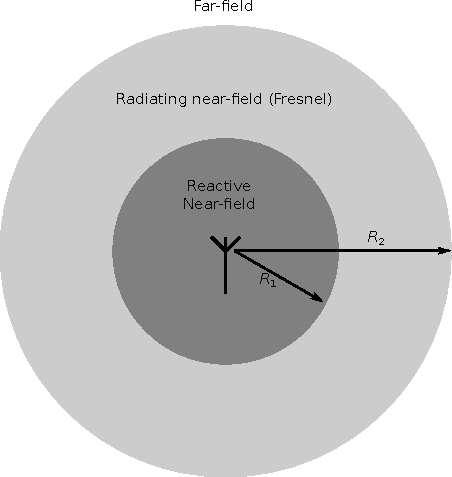
\includegraphics[scale=1]{img/analysis/radiationfields}
  \caption{Visualization of different fields \cite{balanis2012antenna}.}
  \label{fig:field-regions}
\end{figure}

\subsection{Directivity and Gain}
\label{subsec:dir_gain}
Directivity is defined as the ratio of the power radiated at a  point with a certain angle and distance from the antenna compared to what would be radiated from a reference isotropic antenna. Mathematically, it can be written as \cite{balanis2012antenna}: 
\begin{align}
  D = \frac{U}{U_0} = \frac{4 \pi U}{P_{rad}} 
\end{align}
where
\begin{where}
  \item[$D$] directivity
  \item[$U$] radiation intensity
  \item[$U_0$] radiation intensity of an isotropic source
  \item[$P_{rad}$] total radiated power 
\end{where}
It should be noted, that for this equation to be valid, the waves must propagate as plane waves, thus being in the far-field region.

Gain is a measure closely related to directivity, it takes the antenna efficiency of the antenna into account as well as the direction. The gain is defined as the ratio of the intensity in a given direction to the radiant intensity that would be obtained if it was radiated isotropically. In mathematical form it can be expressed as \cite{balanis2012antenna}:
\begin{align}
  G = 4 \pi \frac{\text{radiation intensity}}{\text{total accepted input power}} = 4 \pi \frac{U(\theta,\phi)}{P_{in}}
\end{align}
In many cases the relative gain is used, which is defined as the ratio of the power gain in a given direction to the power gain of a reference antenna in its referenced direction. The reference antenna could be a dipole, horn etc. 

The gain can also be calculated using the directivity, since they are only related by the efficiency. This is given as \cite{balanis2012antenna}:
\begin{align}
  G(\theta,\phi) = e_{cd}D(\theta, \phi) 
\end{align}

\subsection{Impedance, Return Loss, and VSWR}
The impedance and matching is an important part of the antenna design to ensure maximum power transfer. The input impedance of an antenna is defined as $Z_{\text{in}}$. From the classical circuit theory it is known that the maximum power transfer occurs when the in- and output impedance is matched (see Section~\ref{sec:tuners}). If there is a mismatch, some of the power will be reflected back into the source, and thus not transmitted from the antenna. The reflection coefficient $\Gamma$ is defined as \cite{pozar2011microwave}:
\begin{align}
    \Gamma = \frac{Z_{\text{in}}-Z_0}{Z_{\text{in}}+Z_0} 
\end{align}
where
\begin{where}
\item[$Z_0$] denotes the characteristic impedance, which is typically \SI{50}{\ohm}.
\end{where}
The reflection coefficient is furthermore often expressed in \si{dB}. 

Another closely related figure is the Voltage Standing Wave Ratio (VSWR), and is defined as \cite{pozar2011microwave}: 
\begin{align}
  \text{VSWR} = \frac{1+|\Gamma|}{1-|\Gamma|}
\end{align}

\subsection{Bandwidth}
The bandwidth of an antenna defines the usable spectrum of the antenna. The needed bandwidth is dependent on the modulation schemes used, which makes the bandwidth an important part of the antenna design. The bandwidth is defined with respect to a given reflection coefficient or VSWR.

\subsection{Polarization}
The polarization in a certain direction is simply defined as the polarization of the transmitted wave by the antenna. It describes the time-varying direction at relative magnitude of the E-field vector analogously to the polarization of light. Similar to light, the polarization can be classified into groups such as linear, circular, or elliptical polarization. If two antennas are of different polarization, this will introduce a polarization mismatch loss to the system \cite{balanis2012antenna}.

\subsection{Antenna Efficiency}
There are a lot of different measures for antenna efficiency depending on which losses that are taken into account. The total efficiency takes the losses from the input terminal and within the antenna structure \cite{balanis2012antenna}. This can in general be expressed as \cite{balanis2012antenna}
\begin{align}
\label{eq:ant-eff}
  e_0 = e_r e_c e_d 
\end{align}
where
\begin{where}
\item[$e_0$] total efficiency.
\item[$e_r$] mismatch loss.
\item[$e_c$] conduction efficiency.
\item[$e_d$] dielectric loss.
\end{where}
The conduction and dielectric losses are hard to compute, and by measurements they cannot be separated \cite{balanis2012antenna}.

\subsubsection{Radiation Efficiency}
The radiation efficiency is defined as the conduction-dielectric efficiency $e_r = e_{cd}$ which is defined as the ratio of the power delivered to the radiation resistance, $R_r$, to the power delivered to $R_r$ and $R_L$ \cite{balanis2012antenna}. This can be written as \cite{balanis2012antenna}:
\begin{align}
  e_r = \frac{P_{\text{radiated}}}{P_{\text{input}}} = \frac{R_r}{R_L+Rr}
\end{align}

\subsection{Antenna Q Factor}
The antenna Q factor (Quality factor) is often used to get an estimation of the bandwidth of a given antenna. The definition of the Q factor of an antenna is defined in Equation~\ref{eq:antenna-q-factor} below \cite{fundamentalMcLean}: 
\begin{align}
  \label{eq:antenna-q-factor}
      Q =
    \begin{dcases}
       \frac{2 \omega W_e}{P_{\text{rad}}} & W_e > W_m  \\
       \frac{2 \omega W_e}{P_{\text{rad}}} & W_m > W_e 
    \end{dcases}
\end{align}
where 
\begin{where}
\item[$W_e$] the time-average non-propagating stored electric energy.
\item[$W_m$] the same as the above just with magnetic energy.
\item[$\omega$] the radian frequency and $P_{\text{rad}}$ denotes the radiated power.
\end{where}

\section{Mobile Antenna Limitations}
As the requirements for mobile antennas gets more and more strict, some trade off's need to be considered when designing an antenna.
The design constrains when designing antennas is a trade off between size, bandwidth and efficiency, as illustrated in Figure \ref{fig:antenna_tradeoff}. 

The trade off relationship can be expressed as\cite{hilbert2015tradeoff}: 
\begin{align*}
  \frac{\Delta f}{f} \propto \frac{(a/ \lambda)^3}{\eta}
\end{align*}

\begin{where}
\item [$\lambda$] Wavelength.
\item [$\eta$] Efficiency.
\item [$\Delta f / f$] Bandwidth.
\item [$a^3$] Antenna volume.
\end{where}

This relationship expresses that it is very hard, if not impossible, to design a small antenna with excellent efficiency performance and a high bandwidth.
Therefore, when designing mobile antennas that requires high bandwidth and small antenna structures a trade off is needed to ensure that the antenna performs as required\cite{hilbert2015tradeoff}.

In the case of the goal of this project the antenna is desired to have a bandwidth from \SI{690}{MHz} to \SI{960}{MHz} in the low band and from \SI{1710}{MHz} to \SI{2650}{MHz} in the high band. Furthermore it needs to be very small with a ground clearance of \SI{5}{mm} and an efficiency above \SI{50}{\percent} in the entire bandwidth. Due to the constrains on the antenna size, when designed to mobile phones, the bandwidth and efficiency will be limited. This leads to design challenges in exploiting the available and limited volume, within a sphere, the best way possible\cite{balanis2012antenna}.  

As this is very hard to accomplish with a fixed-tuned antenna, a frequency reconfigurable antenna system could be one way of covering a high bandwidth with a small antenna \cite{hilbert2015tradeoff}.  

\begin{figure}[htbp]
  \centering
  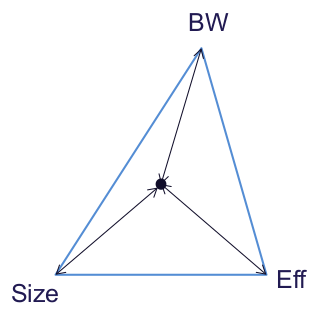
\includegraphics[scale=0.4]{img/analysis/antenna_limitations}
  \caption{Antenna design trade off's}
  \label{fig:antenna_tradeoff}
\end{figure}

\subsection{Electrically Small Antennas}
The concept and definition of electrically small antennas was introduced by Wheeler in 1947 \cite{wheeler1947}, and is given by:
\begin{align}
\label{eq:esa-def}
  ka \ll 1
\end{align}
where 
\begin{where}
\item[$k$] $\frac{2\pi}{\lambda}$ is the wave number. 
\item[$a$] the radius of a sphere enclosing the maximum dimension of the antenna. 
\end{where}
The parameter $a$ is illustrated in Figure~\ref{fig:ant-esa-def}. Inserting the definition of $k$ yields that
\begin{align}
  \frac{2\pi a}{\lambda} \ll 1
\end{align}
in order for an antenna to be defined as electrically small. It should also be noted that, if the antenna is used with a small ground plane, which often is the case, then the ground plane it self becomes a dominant part of the antenna structure. In this case, the entire ground plane must be included in the sphere and thus in the definition of $a$.

\begin{figure}[htbp]
  \centering
  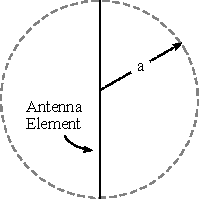
\includegraphics[scale=1]{img/analysis/ESA}
  \caption{Illustration of ESA definition \cite{}}
  \label{fig:ant-esa-def}
\end{figure}

\subsubsection{Fundamental limits of Q}
L.J.\ Chu quantified the relationship between the minimum Q of an electrically small antenna and the physical size relative to the wavelength \cite{chu1948}. This relationship was later corrected by McLean \cite{mclean1996} to be: 
\begin{align}
  Q_L = \frac{1}{k^3a^3}+ \frac{1}{ka}
\end{align}
For a linear antenna in free space and for a circular polarized antenna \cite{mclean1996}:
\begin{align}
  Q_{cp} = \frac{1}{2}  \left[ \frac{1}{k^3a^3} + \frac{2}{ka} \right] 
\end{align}

\subsection{Friis Transmission Equation}
The Friis transmission equation relates the power received with the power transmitted. In the most simple form the Friis transmission equation is based on the Free-space path loss (FSPL), the gains of the antennas and the transmit power. The free-space path loss (or ``path gain'' as this is a negative notation) is defined as \cite{balanis2012antenna}
\begin{align}
  \label{eq:fspl}
  \text{FSPL} = \left( \frac{\lambda}{4 \pi d} \right)^2 
\end{align}
where
\begin{where}
\item[$\lambda$] wavelength.
\item[$d$] distance from the transmitter.
\end{where}
This assumes that the energy spreads out in a sphere and that the only loss is from the distance. It is seen that the power decreases as the square of the range, which is plotted on Figure~\ref{fig:fspl-plot} for a \SI{2.6}{GHz} link.

\begin{figure}[htbp]
  \centering
  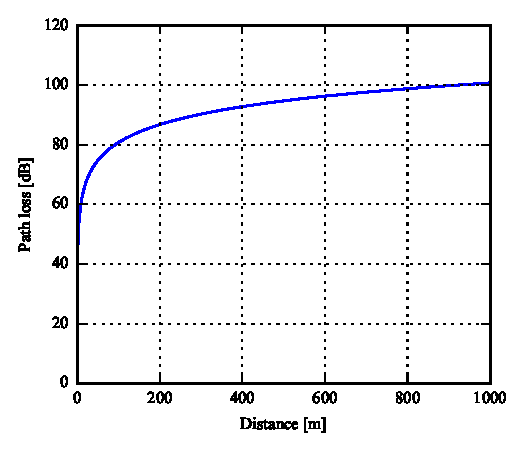
\includegraphics{img/analysis/distancePathloss}
  \caption{Free space path loss in dB for a \SI{2.6}{GHz} link.}
  \label{fig:fspl-plot}
\end{figure}

The Friis Transmission equation in its most basic form can be written as \cite{balanis2012antenna} 
\begin{align}
    \frac{P_r}{P_t} = \left( \frac{\lambda}{4 \pi d} \right)^2 G_{t} G_{r} 
\end{align}
where
\begin{where} 
\item[$P_r$] power received.
\item[$P_t$] power transmitted.
\item[$G$] transmitter and receiver gains.
\end{where}
In this case it is assumed that there is no impedance or polarization mismatch. It is also assumed that the two antennas are aligned perfectly. Another large assumption is that the path loss is described by FSPL, which in reality is a very rare case. The next section will describe a few different propagation models.

\section{Basic Propagation Models}
\label{sec:propmodels}
This section will describe some simple propagation models and terms, that can be used to establish a rough estimate of the losses from propagation, which can be used in link budgets. The simplest propagation model is the Free space path loss, which is given in Equation~\ref{eq:fspl}.

The free-space path loss is however not very realistic, since it does not take trees, buildings etc. into account \cite{balanis2012antenna}. There are however a myriad of empirical models, which are based on actual measurements. The drawback is however that these empirical models tend not to be general and a given model might not be suited for two different cities. This results in that empirical models often are grouped into three main branches, foliage, terrain and city models \cite{goldsmith2005wireless}. For foliage areas models such as the Weissbergers model and the ITU Vegetation model can be used \cite{goldsmith2005wireless}. For terrain areas, models such as the Egli or Longley-Rice model are used \cite{goldsmith2005wireless}. To model the path loss in cities, the Young, Okumura, Hata or the COST 231 models can be used \cite{goldsmith2005wireless}. It should be noted that some of these models are not usable in upper LTE frequency range, and thus care should be taken when applying these models. 


\subsection{Multipath}
The multipath effect exists when a wave and/or multiple waves are scattered, such that the receiver experiences multiple copies of the same wave coming from different directions. In areas where there is no ground or other obstacles (free space) the multipath effect does not exist. The simplest multipath case is the two-ray case, where the surface of the earth is included, in this case there will be a single reflection from the earth and thus multiple paths from the transmitter to receiver \cite{parsons2000mobile}. This scenario is illustrated in Figure~\ref{fig:mul_tworay}.
 
\begin{figure}[htbp]
    \centering
    \begin{subfigure}[b]{0.6\textwidth} 
        \centering
        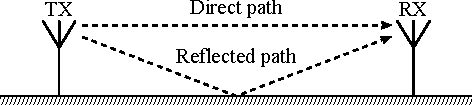
\includegraphics{img/analysis/tworay}
        \caption{Two ray path model.}
        \label{fig:mul_tworay}
    \end{subfigure}
    \\
    \begin{subfigure}[b]{0.7\textwidth} 
        \centering
        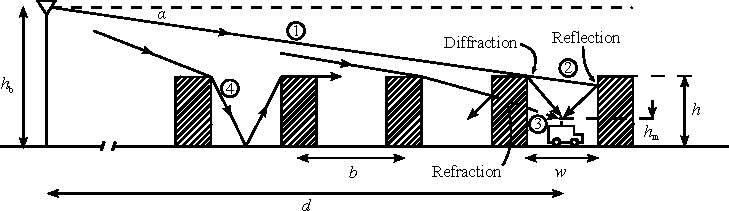
\includegraphics{img/analysis/parsons_multipath}
        \caption{Reflection and diffraction causing the multi-path effect \cite{parsons2000mobile}. The signal received by the car consists of diffracted, reflected, and refracted waves but no direct line-of-sight component.}
        \label{fig:mul_reflec_diffrac}
    \end{subfigure}
    \caption{Two ray model and different multipath effects.}
\end{figure}

The multipath effect will be greatest in urban environments, where several buildings and other obstacles are present. If the surface is rough, scattering will also take place. This is the phenomenon where a single incoming wave scatters into multiple reflections. In addition to this there is also diffraction where a wave front is ``bend'' at the edges of buildings which is illustrated in Figure~\ref{fig:mul_reflec_diffrac}. Multipath results in a negative effect on the throughput. However, with MIMO, the multipath effects are now exploited positively to increase throughput and channel stabilization \cite{parsons2000mobile}.

\subsection{Fading}
The signal strength in a wireless channel is constantly fluctuating. These variations are represented by fading. The variations can be caused by scattering, reflections, blockage etc. Based on the type of variation the fading is grouped in \emph{small scale fading} and \emph{large scale fading}. Large scale fading is typically caused by large objects, such as hills and buildings, where small scale fading occurs over small travel distances due to constructive or destructive adding of the multipath waves \cite{parsons2000mobile}.

By superimposing the path loss with small scale fading and large scale fading, the combined model is obtained which represents the total propagation and path loss model. This is illustrated in Figure \ref{fig:mul_combined}. 

\begin{figure}[htbp]
    \centering
    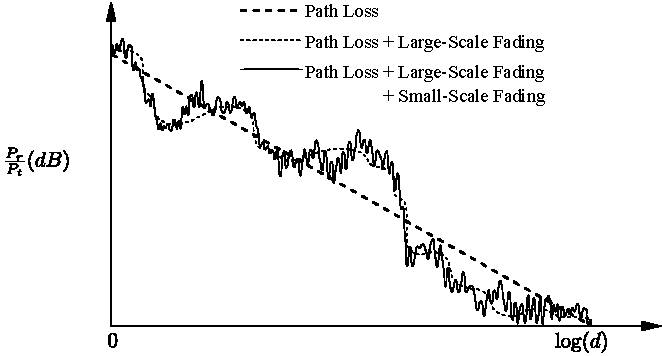
\includegraphics{img/analysis/goldsmith_combined}
    \caption{Combined path loss model with large- and small-scale fading \cite{goldsmith2005wireless}.}
    \label{fig:mul_combined}
\end{figure}

\subsection{Empirical Models}
This section will describe some of the city-models, that are often used in estimating the pathloss. 

\subsubsection{Hata Model}
The Hata model is a mathematical model derived from the graphically Okumura model, which is based on measurements from Tokyo in 1960 in the frequency range \SIrange{200}{1920}{MHz}. The model is divided into three groups: Urban, suburban, and open areas which are defined in dB in Equation~\ref{eqn:hataModelUrban}, Equation~\ref{eqn:hataModelSubUrban}, and Equation~\ref{eqn:hataModelOpen} respectively \cite{Seybold2005introduction}.
\begin{align} 
    \label{eqn:hataModelUrban}
    L_{50} = L_{50}(\text{urban}) = 69.55+26.12 \log(f_c) - 13.28 \log(h_t) -a(h_r) + [44.9-6.55 \log(h_t)] \log(d)
\end{align} 
where
\begin{where}
\item [$f_{c}$] Center frequency in \si{MHz} and in the range: $150 < f_c < 1500$
\item [$h_t$] Height in meters, which must satisfy $30 < h_t < 200$
\item [$d$] Distance in km which must satisfy $1 < d < 20$
\item [$a(h_r)$] The mobile antenna height correction factor. Defined in Equation~\ref{eqn:hataModelahrSmall} \cite{Seybold2005introduction} for small and medium sized cities. Defined in Equation~\ref{eqn:hataModelahrLarge} \cite{Seybold2005introduction} for a large city. 
\end{where}
\begin{align} 
\label{eqn:hataModelahrSmall}
a(h_r) &= [1.1 \log(f_c)-0.7]h_r - [1.56 \log(f_c)-0.8]\quad\text{if } \SI{1}{m} \leq h_r \leq \SI{10}{m} \\
\label{eqn:hataModelahrLarge}
a(h_r) &= 
  \begin{cases}
    8.29[\log(1.54 h_r))^2 -1.1 & \text{ if } f_c \leq \SI{200}{MHz}, \\
    3.2[\log(11.75 h_r))^2 -4.97 & \text{ if } f_c \leq \SI{400}{MHz} 
  \end{cases}\\
\label{eqn:hataModelSubUrban}
L_{50} &= L_{50}(\text{urban})-4.78[\log(f_c)]^2 + 18.33 \log(f_c) - 40.94 \\
\label{eqn:hataModelOpen}
L_{50} &= L_{50}(\text{urban})-2 \left[\log\left( \frac{f_c}{28} \right) \right]^2 -5.4 
\end{align} 
This extension to the Okumura model is often used in practical applications since it is easier to apply than the Okumura model. However, it only handles frequencies up to \SI{1500}{MHz}, which lead to the COST 231 model being developed. 

\subsubsection{COST 231 Model}
%COST 231 Model
The COST 231 model is an extension of the Hata model. It includes the PCS bands \SIrange{1800}{1900}{MHz} which makes it an ideal model for many wireless personal communication systems (GSM etc.). The path loss is given by Equation~\ref{eqn:COSTModel} in dB \cite{Seybold2005introduction} and the model is valid in the frequency range of  \SIrange{1500}{2000}{MHz}, link distance of up to \SI{20}{km}, a transmitter antenna height of \SIrange{30}{200}{m}, and a receiver height of \SIrange{1}{10}{m} \cite{Seybold2005introduction}. It should also be stated that the model is restricted to applications where the base station antenna is above adjacent roof tops \cite{itu2002report}.
\begin{align} 
    \label{eqn:COSTModel}
    L_{50} = 46.3+33.9 \log(f_c)-13.82 \log(h_t)-a(ht)+[44.9-6.55 \log(h_t)] \log(d) + C 
\end{align} 
where 
\begin{where}
\item [$f_c$] The frequency in \si{MHz}.
\item [$h_t$] Transmitter height in \si{m}. 
\item [$h_r$] Receiver height in \si{m}.
\item [$a(h_r)$] The mobile antenna height correction factor from Equation~\ref{eqn:hataModelahrSmall} and Equation~\ref{eqn:hataModelahrLarge}.
\item [$d$] Distance of propagation.
\item [$C$] \SI{0}{dB} for suburban and medium cities with medium tree density, 3 dB for metropolitan centers. 
\end{where}

\subsubsection{Extended COST}
%Extended COST 
An extension to the COST 231 model is described in a ITU (International Telecommunication Union) report \cite{itu2002report} and this model extends the COST 231 such that it is accurate up to \SI{3}{GHz}. The path loss model for an urban environment in the range of \SIrange{2000}{3000}{MHz} is given by \cite{itu2002report}
\begin{equation} 
\label{eqn:COSTModelExtended}
\begin{aligned}
    L &= 46.3 + 33.9 \log(2000) + 10 \log\left(\frac{f_c}{2000}\right) \\
        &- 13.82 \log(\text{max}\{30,h_t\}) + [44.9 -6.55 \log(\text{max}\{30,h_t\})] (\log(d))^{\alpha} - a(h_r) - b(h_t)
%L = 46.3 + 33.9\log(2000) + 10\log(\frac{f_c}{2000}) − 13.82\log(max{30,H_t}) +[44.9 − 6.55\log(max{30,H_t})](\log(d))\alpha −a(H_r)−b(H_t)
\end{aligned}
\end{equation} 
where 
\begin{where}
\item [$f_c$] The frequency in \si{MHz}.
\item [$h_t$] Transmitter height in \si{m}. 
\item [$h_r$] Receiver height in \si{m}.
\item [$a(h_r)$] The mobile antenna height correction factor given in Equation~\ref{eqn:COSTModelExtendedhr}
\item [$b(h_t)$] Transmitter height correction factor given in Equation~\ref{eqn:COSTModelExtendedht}
\item [$\alpha$] Given in Equation~\ref{eqn:aplhacostextended}.
\end{where}
\begin{align} 
\label{eqn:COSTModelExtendedhr}
a(h_r)&=(1.1\log(f)-0.7) \min\{10,h_r\}-(1.56\log(f)-0.8)+\max\left\{0,20\log\left(\frac{h_r}{10}\right)\right\}\\
\label{eqn:COSTModelExtendedht}
b(h_t)&= \min\left\{0,20\log\left(\frac{h_t}{30}\right)\right\}\\
\label{eqn:aplhacostextended}
\alpha &= 
  \begin{cases}
      1 & \text{ if } (d \leq \SI{20}{km}) \\
    1+(0.14+1.87e^{-4} f + 1.07e^{-3} h_t & \text{ if } (\SI{20}{km} < d \leq \SI{100}{km})
  \end{cases}
\end{align} 

\section{MIMO in Handsets}
\label{sec:mimo_in_handsets}
\begin{aautop}
Multiple antennas in both transmitter and receiver in wireless systems, which is better known as MIMO, has become a widespread technology and used in many applications today, due to its ability to increase performance. Most wireless systems are limited by the channel in which they propagate, due to phenomenons such as multi-path fading. Multi-path happens when the transmitted signal travels through multiple different paths, which influences the time it takes for the signal to reach the receiver, the angle of arrival, and even frequency shifts due to Doppler. This creates random fluctuation in the received signal level, affecting the performance of the wireless communication. MIMO is an effective way of dealing with the challenges in delivering more throughput and coupe with the multipath effects from buildings. MIMO exploits the multi-path phenomenon to transmit several different data streams simultaneously, also referred to as spatial multiplexing. This can help in both single user or in multi-user scenarios. For the single user, it allows for faster data rates without increasing the transmit power or allocating more frequency resources. In the multi-user scenario, the base station can effectively create beams to individual users while using the same shared frequency. This is also known as Space Division Multiple Access (SDMA). The purpose of this section is to explain what is understood by such a system, how it relates to the antenna design, and how it makes a difference. The principal mechanisms and performance metrics are explained. This section will not describe the statistical channel models but rather focus on the antenna related perspectives.
\end{aautop}

\begin{figure}[htbp]
  \centering
  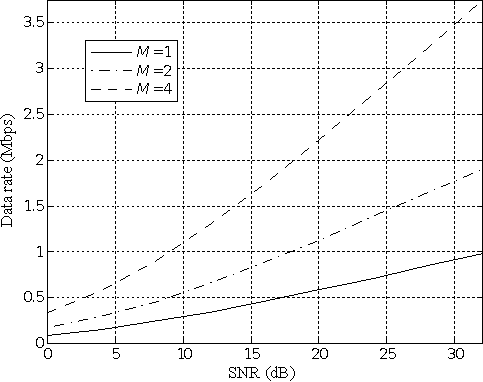
\includegraphics[scale=1.2]{img/analysis/datarateMimo}
  \caption{Throughput versus SNR given a specific M-ary MIMO-setup \cite{Ezio2007MIMO}.}
  \label{fig:mimo-throughput}
\end{figure}

\subsection{Perks of MIMO} 
As shown in the introduction to this section, the use of MIMO results in enhanced performance. Figure~\ref{fig:mimo-throughput} shows the general performance increase, however this is gained by the addition of multiple different performance gains. The performance gains are spatial diversity gain, multiplexing gain, array gain, and interference reduction \cite{Ezio2007MIMO}, which will be described briefly in the following.

\subsubsection{Spatial Diversity Gain}
The spatial diversity gain improves the resistance to fading in the receiver. This is done by providing the receiver with multiple different copies of the same transmitted signal. Ideally, the copies are independent from another. A diversity technique is required to combine the signals at the receiver \cite{Ezio2007MIMO}. Some examples could be equal gain combining, maximal-ratio combining, or selection combining. The spatial diversity is also quite intuitive since the probability that one of the signals are not in a fade increases per added element, given that they are somewhat independent. 
 
\subsubsection{Spatial Multiplexing Gain}
Spatial multiplexing can be used in scatter rich channels where the received signals are independent. Instead of transmitting the same signal, as done in diversity gain, the spatial multiplexing transmits multiple independent data streams. This allows for a linear increase in the data rate, thus the capacity of the wireless network is increased. Generally, the number of independent streams that can be supported is limited by the number of receive antennas \cite{Tim2012Practical}.

\subsubsection{Array Gain}
The array gain is the result of coherent combining of the wireless signals at the receiver, which results in an increase in the receive SNR. The array gain is improved linearly as the number of receive antennas increases \cite{tse2005fundamentals}. This gain improves the resistance to noise and thus also the coverage \cite{Tim2012Practical}.
  
\subsubsection{Interference Gain}
By using MIMO, the interference from different users and base stations can be avoided by exploiting extra spatial degrees of freedom, such as array gain. Furthermore, beam-steering could be implemented such that the signal could be directed towards the designated receiver. Obviously, all of the above can not be used at the same time. However, using a combination allows for improved coverage, capacity, and reliability \cite{Tim2012Practical}.

\subsection{Channel Capacity}
\def\snr{\text{SNR}_{\text{AWGN}}}
\def\PP{\overline{P}}
\def\CC{C_{\text{AWGN}}}

The capacity of a channel is the maximal transmission rate for which a reliable communication can be achieved, and if the transmission rate exceeds this, the system breaks down \cite{Tim2012Practical}. The channel capacity is one of the primary performance measures to characterize the performance of MIMO systems \cite{Tim2012Practical}. This section will focus on the capacity for time-invariant SISO, SIMO, MISO, and MIMO channels. The main assumptions for the time-invariant channel is the following \cite{Tim2012Practical}: 
\begin{itemize}
\item The channel is time-invariant.
\item A codeword spans over an asymptotic long data block, which averages out the noise.
\item Channel state information is available at both the transmitter and receiver. 
\end{itemize}

\subsubsection{Time-Invariant SISO Channel}
A simple SISO channel, as illustrated in Figure~\ref{fig:sisoModel}, is given by the input-output relation:
\begin{align*} %%
  y(k) = h x(k) + n(k)
\end{align*}

Here $h$ describes the channel, which is time \emph{independent}. The signal power is $\PP |h|^2$, which is the power in $h x(k)$ and the noise power of $n(k)$ is $\sigma_n^2$. Thus, the SNR is given by the ratio \cite{Tim2012Practical}
\begin{align} %%
  \snr = \frac{\PP |h|^2}{\sigma_n^2}
\end{align}
This yields a channel capacity of \cite{Tim2012Practical} 
\begin{align} %%
      \CC &= \log_2 \left( 1 + \snr \right)
\end{align}
It is seen that the SNR is an important factor for the AWGN channel capacity.
\begin{figure}[hbp]
  \centering
  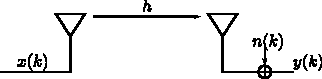
\includegraphics[scale=1.2]{img/analysis/sisoModel}
  \caption{The time-invariant SISO channel}
  \label{fig:sisoModel}
\end{figure}

\subsubsection{Time-Invariant SIMO Channel}
The channel capacity for a SIMO system, where a symbol $x(k)$ is sent from a single antenna and received at $M_R$ antennas, is illustrated in Figure~\ref{fig:simoModel}. In a SIMO system, the signal is coherently combined at the receiver. When including this post-processing, the system transforms into an equivalent SISO channel \cite{Tim2012Practical}.

\begin{figure}[htbp]
  \centering
  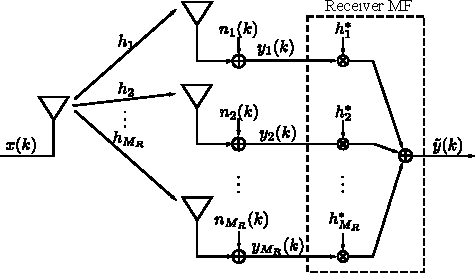
\includegraphics[scale=1.2]{img/analysis/simoModel}
  \caption{The time-invariant SIMO channel.}
  \label{fig:simoModel}
\end{figure}

The system model changes from a scalar equation to a vector notation due to the multiple antennas. The channel coefficients are denoted as $h_j$, $j,\ldots,M_R$ and are known at the transmitter. At a given antenna, $j$, the received signal $y_j(k)$ is given by \cite{Tim2012Practical}: 
\begin{align} %%
  y_j(k) = h_j x(k) + n_j(k)
\end{align}

The multiple antennas receive multiple distorted copies of the transmitted symbol. Each received signal, has different parts of the signal depending on the channel. To recover most of the original message, the different symbols are combined. This combination can be done in multiple ways: Matched filtering, maximum ratio combining, or equal-gain combining. Matched filtering requires the most amount of post-processing since it requires the signals to be aligned in phase, so they can be added constructively and scaled. This maximizes the post-processing SNR of the SIMO system. Mathematically the received signal at antenna $j$ is first multiplied with a scalar coefficient $h_j^*$ matched to the channel. This yields $|h_j|^2 x(k) + h_j^* n_j(k)$. The processed signals are then added up, resulting in a processed signal \cite{Tim2012Practical} 
\begin{align}%%
  \tilde{y}(k) = \norm{\mathbf{h}}^2 x(k) + \tilde{n}(k)
\end{align}

The SIMO system becomes equivalent to a scalar AWGN channel, with a potentially larger SNR due to the post-processing \cite{Tim2012Practical}. This leads us to an SNR and a channel capacity given by \cite{Tim2012Practical}
\begin{align} %%
\text{SNR}^{\text{TI}}_{\text{SIMO}} &= \frac{\PP \norm{\mathbf{h}}^2}{\sigma^2_n} \\
C^{\text{TI}}_{\text{SIMO}} &= \log_2 \left( 1+\frac{\PP \norm{\mathbf{h}}^2}{\sigma^2_n} \right)  
\end{align}

\subsubsection{Time-Invariant MISO Channel}
In the MISO case, the system consists of multiple antennas at the transmitter and a single antenna at the receiver. This is illustrated in Figure~\ref{fig:misoModel}.
\begin{figure}[htbp]
  \centering
  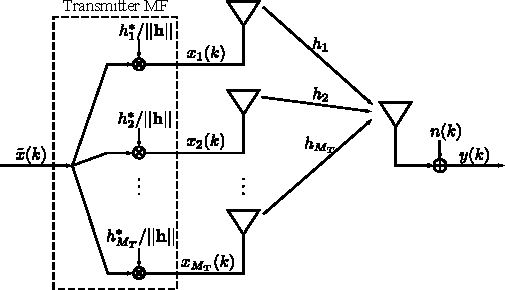
\includegraphics[scale=1.2]{img/analysis/misoModel}
  \caption{The time-invariant MISO channel.}
  \label{fig:misoModel}
\end{figure}
Given that the channel is known at the transmitter, it is possible to perform pre-processing on the transmitted signals. This transforms the MISO case in to an equivalent SISO channel. The pre-processing consists of scaling each version of the transmitted symbol to insure that the signals are added up constructively at the receiver. The pre-processing must take the channel for each antenna into account when doing this scaling. 

A signal $x_i(k)$ is sent from the $i$th antenna in the array. This signal travels through the channel $h_i$ and this channel is known at the transmitter. The received signal is then given as \cite{Tim2012Practical}: 
\begin{align}%%
  y(k) = \sum_{i=1}^{M_T} h_ix_i(k) + n(k) = \mathbf{h}^\intercal \mathbf{x}(k) + n(k)
\end{align}
where
\begin{where}
  \item[$M_T$] The number of transmitter antennas.
  \item[$\mathbf{h}$] $[h_1 \cdots h_{M_T}]^T$.
  \item[$\mathbf{x}$] $[x_1(k) \cdots x_{M_T}(k)]^T$.
\end{where}

The MISO becomes an equivalent SISO channel. The pre-processing that is often used is transmit spatial matched filtering or transmit MRC, where the transmitted signal is matched to the channel $h_i$ before being sent from antenna $i$. The weights applied in the transmit MF are the exact same as the receiver MF due to perfect knowledge of the channel \cite{Tim2012Practical}. The output of the pre-processing is under the power constraint $\sum_{i=1}^{M_T} E|x_i(k)|^2 \leq \PP$. The signal $x_i$ sent from the antenna is then \cite{Tim2012Practical}
\begin{align}%%
  x_i(k) = \frac{h_i^*}{\norm{\mathbf{h}} \tilde{x}(k)}
\end{align}

On the receiving side, the signals are phase-aligned and added constructively. It is obvious that more power is allocated to the stronger channels, thus maximizing the SNR. The SNR and channel capacity then becomes \cite{Tim2012Practical}:
\begin{align} %%
\text{SNR}^{\text{TI}}_{\text{MISO}} &= \frac{\PP \norm{\mathbf{h}}^2}{\sigma^2_n} \\
C^{\text{TI}}_{\text{MISO}} &= \log_2 \left( 1+\frac{\PP \norm{\mathbf{h}}^2}{\sigma^2_n} \right)  
\end{align}
Thus, it is seen that for time-invariant channels with perfect channel knowledge for both transmitter and receiver, the capacity for SIMO and MISO systems are the same. This is, however, not the case for fading channels when the channel state is unknown for the transmitter. This leads to performance degradation in the MISO case \cite{Tim2012Practical}. 

\subsubsection{Time-Invariant MIMO Channel}
When multiple antennas are available at both transmitter and receiver, the capacity can be increased by sending multiple symbols per transmission period. This relies on pre- and post-processing which is matched to singular value decomposition of the channel \cite{Tim2012Practical}, illustrated in Figure~\ref{fig:mimoModel}. This processing extracts independent spatial routes for the communication. MIMO can be interpreted as multiple pairs of independent SISO channels where the capacity simply becomes the sum of these independent SISO channels \cite{Tim2012Practical}.

\begin{figure}[htbp]
  \centering
  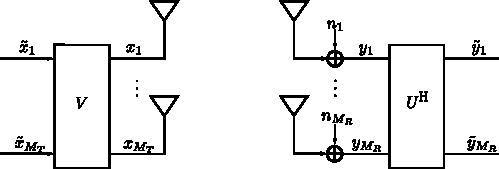
\includegraphics[scale=1.2]{img/analysis/mimoModel}
  \caption{The time-invariant MIMO channel.}
  \label{fig:mimoModel}
\end{figure}

The singular value decomposition of the channel matrix is fundamental in understanding the underlying concepts of MIMO systems. The SVD extracts the equivalent independent AWGN channels, gives the maximum number of streams that can be multiplexed, and it provides a simple way to compute the capacity. The SVD of the channel matrix $\mathbf{H}$ is \cite{Tim2012Practical}
\begin{align}%%
  \mathbf{H} = \mathbf{U} \Lambda \mathbf{V}^{\mathsf{H}} 
\end{align}
 
Both $\mathbf{U}$ ($M_R \times \ M_R$) and $\mathbf{V}$ ($M_T \times \ M_T$) are unitary matrices, and $\Lambda$ is a  $M_R \times \ M_T$ diagonal matrix with non-negative singular values $\lambda_k$ with $k=1, \cdots, M_{\text{min}}$ where $M_{\text{min}} = \min(M_T,M_R)$. The $\lambda_k$'s are called the eigenmodes of the channel and are often ordered decreasingly for convenience.

Another important quantity is the channel matrix rank $\mathbf{H}$, which is denoted $r_H$. This is defined as the number of nonzero singular values of $\mathbf{H}$, which determines the maximum number of independent streams that can be multiplexed at the same time \cite{Tim2012Practical}. The singular value and channel energy relationship is also useful. This is given as 
\begin{align} %%
  \text{tr}(\mathbf{H} \mathbf{H}^{\mathsf{H}}) = \sum_{i=1}^{M_T} \sum_{j=1}^{M_R} |h_{ji}|^2 = \sum_{k=1}^{r_H} \lambda_i^2
\end{align}
Each channel is called an eigenchannel. The entire MIMO channel is equivalent to the set of eigenchannels, each with a different SNR. Looking at the input-output relation \cite{Tim2012Practical}
\begin{align}%%
  \tilde{y} = \Lambda\mathbf{ \tilde{x}} + \mathbf{\tilde{n}}
\end{align}
From each input-output relation $\tilde{y}_k = \lambda_k \tilde{x}_k + \tilde{n}_k$ it is obvious that this describes an AWGN channel as seen previously in the SISO case. Since the noise are all independent, each AWGN subchannel are all independent as well. This forms a set of parallel AWGN channels, which leads to the conclusion that the capacity of the MIMO system is the sum of individual channel capacities. Finally, it is needed to include the transmit power allocation to fully calculate the channel capacity.

The power allocation is done using the water-filling algorithm \cite{Tim2012Practical}. For each eigenchannel we define: 
\begin{align}%%
  \gamma_k = \frac{\lambda_k^2}{\sigma_n^2}, \text{where } k = 1, \cdots, r_h
\end{align}
The transmitted power of eigenchannel $k$ is given by $P_k$. Then $P_k\gamma_k$ can be interpreted as the SNR of the $k$th eigenchannel. The capacity of each eigenchannel with transmit power $P_k$ becomes $\log_2 (1 + P_k\gamma_k)$. Now, this becomes a maximization problem, in which the SNR or channel capacity should be maximized with respect to the power constraint: $\sum_{k=1}^{r_H} P_k \leq \PP$. 
The channel capacity of the MIMO system is then the sum of the individual capacities with optimized transmit power per eigenchannel \cite{Tim2012Practical}
\begin{equation}%%
\begin{aligned}
C^{\text{TI}}_{\text{MIMO}} = 
& \underset{P_k}{\text{maximize}}
& & \sum_{k=1}^{r_H} \log_2 (1 + P_k\gamma_k) \\
& \text{subject to}
& & \sum_{k=1}^{r_H} P_k \leq \PP
\end{aligned}
\end{equation}
This optimization problem can be solved using the Lagrangian multipliers method, which gives the capacity of the time-invariant MIMO channel as \cite{Tim2012Practical} 
\begin{align}%%
  C^{\text{TI}}_{\text{MIMO}} = \sum_{k=1}^{r_H} \log_2 (1 + P^o_k\gamma_k)
\end{align}
where the transmit power is allocated as
\begin{align}
  P_k^o = \big(\frac{1}{\gamma_0} - \frac{1}{\gamma_k}\big)^+ 
\end{align}
Here, $y_0$ is the cut-off value and it is determined using the power constraint
\begin{align}%%
  \sum_{k=1}^{r_H} P_k^o = \sum_{k=1}^{r_H} \big(\frac{1}{\gamma_0} - \frac{1}{\gamma_k}\big)^+ = \PP
\end{align}

From this it is seen that the power allocation and channel matrix rank are key elements to MIMO. The major advantage for MIMO systems is the fact that multiple streams of data can be sent simultaneously. The MISO and SIMO systems only experience an increase in SNR which allows for a more robust channel and the use of higher order modulation schemes. However, this is only true for independent AWGN channels, and in reality, the channel capacity has to be expressed scholastically using complex channel models.  

\subsection{Antenna Design in MIMO Applications}
\label{sec:mimoant}
The three most important factors in MIMO antenna design are: Near-field coupling, the envelope correlation $\rho_e$, and total efficiency $\eta_{\text{total}}$. The near-field coupling is a measure of the coupled power towards the second antenna when the first antenna is excited. The coupling is evaluated by the $S_{21}$ parameter and is often referred to as the \emph{isolation}. This isolation affects the efficiency and envelope correlation coefficient \cite{Tatomirescu2011PortIsolation}. The envelope correlation coefficient is a measure of how independent the antenna radiation patterns are, so if the two radiation patterns are pointing in two different directions, the correlation coefficient is zero, and if the radiation patterns are exactly the same, the correlation coefficient will be one. As a rule of thumb, a correlation coefficient of \num{0.5} is assumed to be sufficient, and \num{0.3} is generally seen as good for MIMO applications \cite{Tim2012Practical}.

The total efficiency is simply given by Equation~\ref{eq:mimo_total_eff} \cite{Tatomirescu2011PortIsolation}, where $\eta_{\text{rad}}$ is the radiation efficiency, which takes dielectric and conductive losses into account.
\begin{align} 
\label{eq:mimo_total_eff}%%
\eta_{\text{total}}=\eta_{\text{rad}} (1-|S_{11}|^2 - |S_{21}|^2)
\end{align}
In practice, the total efficiency may be found directly by supplying a known amount of power to the antenna and observing the power radiated by the antenna. The total efficiency is then the ratio of the radiated power to the supplied/total power \cite{balanis2012antenna}
\begin{align}
    \label{eq:mimo_total_eff_satimo}%%
    \eta_{\text{total}} = \frac{P_{\text{rad}}}{P_{\text{total}}}
\end{align}
The radiated power is proportional to the spherical integral of the farfield obtained in an anechoic chamber \cite{balanis2012antenna}
\begin{equation}
    \label{eq:mimo_prad}%%
    P_{\text{rad}} \propto \intsphere{|F_{\theta}|^2 + |F_{\phi}|^2}
\end{equation}
where $F$ is the complex field sampled for each polarization. The total power, $P_{\text{total}}$, can be found (relatively) by rearranging Equation~\ref{eq:mimo_total_eff_satimo} and using Equation~\ref{eq:mimo_prad} \emph{on a reference antenna} with known total efficiency, $\eta_{\text{total}}^{\prime}$ (here, $^{\prime}$ denotes the reference antenna)
\begin{equation}
    \label{eq:mimo_ptot}
    P_{\text{total}} \propto \frac{P_{\text{rad}}^{\prime}}{\eta_{\text{total}}^{\prime}}
\end{equation}
As both the radiated power and the total power is now found using the same relative power measure (the same radiated-power formula, Equation~\ref{eq:mimo_prad}), the total efficiency can be found using Equation~\ref{eq:mimo_total_eff_satimo}.

The envelope correlation coefficient can be calculated by Equation~\ref{eq:envlop_corr} \cite{Wang2010}. The far-field radiation pattern, $F$ for each polarization, needs to be measured in order to reliably calculate the envelope correlation coefficient.
\begin{align} %%
\label{eq:envlop_corr}
\rho = 
\left|  
%
\frac
{\intsphere{A_{12}(\theta,\phi)}}
{\sqrt{\intsphere{A_{11}(\theta,\phi)} \intsphere{A_{22}(\theta,\phi)}}}
%
\right|^2
\end{align}
where
\def\xpr{\text{XPR}}
\begin{where}
\item[$A_{mn}$]
    $
    \xpr_{mn} \cdot E_{\theta,m}(\theta,\phi) E^*_{\theta,n}(\theta,\phi) P_{\theta}(\theta,\phi)
    +
    E_{\phi,m}(\theta,\phi)E^*_{\phi,n}(\theta,\phi)P_{\phi}(\theta,\phi)
    $.
\item[$E_{x,m}(\theta,\phi)$] The recorded complex farfield in the polarization $x$ of antenna $m$.
\item[$P_x(\theta,\phi)$] The distribution of incoming waves for polarization $x$. If the distribution is assumed to be isotropic, this can be set to $1/4\pi$.
\item[$\xpr_{mn}$] Cross polarization ratio $= P_{v,m}/P_{h,n}$ for the antenna set $mn$.
\item[$P_{v,m}$] Relative power in the $\theta$ polarization of antenna $m$, 
    \begin{equation*}
        P_{v,m} = \intsphere{|E_{\theta,m}|^2}
    \end{equation*}
\item[$P_{h,n}$] Relative power in the $\phi$ polarization of antenna $n$,
    \begin{equation*}
        P_{h,n} = \intsphere{|E_{\phi,n}|^2}
    \end{equation*}
\end{where}

The envelope correlation coefficient can also be estimated by the S-parameters, as given in Equation~\ref{eq:envlop_corr_Sparams} \cite{Alain2010MIMO}. However, the use of this is often discouraged since it assumes very high radiation efficiency \cite{Alain2010MIMO}.
\begin{align} %%
\label{eq:envlop_corr_Sparams}
  \rho_e \approx |\rho_c|^2 = \frac{|S^*_{11}S_{12}+S^*_{21}S_{22}|^2}{(1-|S_{11}|^2-|S_{21}|^2)(1-|S_{22}|^2-|S_{12}|^2)}
\end{align}
Thus, when designing antenna for the purpose of MIMO, the antennas need to be designed in a way such that the elements receives de-correlated signals. This can be done in different ways, such as changing the angular patterns, changing the polarization of the elements, or spatially separating the antennas, which are the most used methods. However, there are also other techniques such as decoupling networks, parasitic elements, active antenna cancellation, eigenmodes, and balanced currents. 


\subsubsection{Spatial Correlation}
The spatial correlation between two antennas is given by the radiated E-field patterns as given in Equation~\ref{eq:envlop_corr}. There, it is seen that the correlation is a comparison between the radiated E-field patterns and the incident E-fields arriving at the antenna, which is given by the probability $P_\theta$ and $P_\phi$.

From the Equation~\ref{eq:envlop_corr} it can also be deduced that the spacing, polarization, and radiation patterns effects the correlation between two antennas. In order to investigate only the effects of spacial separation, we consider the case with two omnidirectional antennas which are both vertically polarized. This is described by Equation~\ref{eqn:spactial_corr} \cite{Tim2012Practical}.
\begin{align} %
\label{eqn:spactial_corr}
  \rho = \oint e^{j\beta \sqrt{d^2+l^2}\cos\zeta}p_\theta(\theta,\phi)\sin\theta \, d \theta d \phi
\end{align}
\begin{where}
\item[$d$] is the horizontal spacing
\item[$l$] is the vertical spacing
\item[$\cos \zeta$] $= \sin(\phi + \tan^{-1}(l/d)\ \text{sgn}\phi)\sin\phi$   
\end{where}

In Figure~\ref{fig:mimo-spacing}, two cases of Equation~\ref{eqn:spactial_corr} are shown: One where only the horizontal spacing is considered and another where only the vertical spacing is considered. The AoA (angle of arrival) is given by Taga and assumes that the AoA in azimuth is uniform and Gaussian in the elevation plane \cite{Tim2012Practical}. The mean angle, $\overline{\theta}$, is at \SI{70}{\degree} and the standard deviation $\sigma_\theta$ is \SI{20}{\degree}. From the plot it can be seen that the vertical spacing required for a certain correlation is larger than that of the horizontal spacing. This comes from the Taga-model used for the angle of arrival, since its distribution is nonuniform. This can, however, not be used to argue that the antennas should be spaced horizontally since smartphones are often operated both horizontally and vertically \cite{Tim2012Practical}. 

It is also possible to make the array in other topologies such as planar, circular, or random. This is, however, not very practical for mobile devices given the current usage of low frequencies in telecommunication (\SIrange{500}{2700}{MHz}) as described in Section~\ref{sec:lte}.

\begin{figure}[htbp]
  \centering
  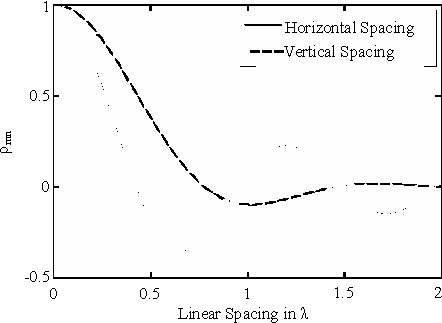
\includegraphics[scale=1.2]{img/analysis/mimoSpacing}
  \caption{Spacing versus wavelength for the horizontal and vertical case\cite{Tim2012Practical}}
  \label{fig:mimo-spacing}
\end{figure}

\subsubsection{Polarization and Radiation Patterns}
In addition to the spatial separation to decorrelate antennas, polarization and different radiation patterns can also be used to decorrelate elements. This is very often used in small mobile devices where the physical size limits the spacing between elements.  

In theory, using a perfectly polarized dipole and loop antenna, it would be possible to create totally decorrelated elements because they have opposite polarization. This is hard to implement in practice, but it is possible to lower the correlation of to elements by having a difference in polarization. However, using different polarization to get a lower correlation requires a suitable XPR in the channel. The XPR should be around \SI{6}{dB} or lower\cite{Tim2012Practical}. 

\subsubsection{Multiplexing Efficiency}
\label{sec:muxefficiency}

Multiplexing efficiency is a measure of total efficiency for an antenna system, taking into account the total efficiency for each antenna \emph{and} the correlation between antenna elements. In this way, it is a single parameter that describes the total loss in SNR (or power) when using a MIMO antenna system \cite{tian2011multiplexing}.

For a $2\times2$ MIMO system, relevant to this project, and assuming high SNR, the multiplexing efficiency, $\eta_{\text{mux}}$, is computed as \cite{tian2011multiplexing}
\begin{equation} %%%%
    \eta_{\text{mux}} = \sqrt{\eta_1 \eta_2 (1 - |\rho|^2)}
\end{equation}
where
\begin{where}
\item[$\eta_n$] Total efficiency of the $n$th antenna.
\item[$\rho$] Correlation between antenna 1 and 2.
\end{where}

In the rest of the report, efficiency and correlation will mostly be treated separately to see more details between the antennas. However, the metric of multiplexing may be useful when evaluating the antennas performance in a link budget.

\section{Matching Circuits and Tuners}
\label{sec:tuners}

% Transmission line theory (reflection, max power transfer)
% [1] Pozar pp 56--57
% [2] Ebert p 29
% [3] Pozar pp 77--78
From transmission line theory, it is known that the voltage and current waves present on a transmission line is composed of an incident and a reflected wave. The voltage and current at any distance, $z$, from the load are \cite{pozar2011microwave}:
\begin{align}
    V(z) &= V^+e^{-j\beta z} + V^-e^{j\beta z}\\
    I(z) &= \frac{V^+}{Z_0} e^{-j\beta z} - \frac{V^-}{Z_0} e^{j\beta z}
\end{align}
where
\begin{where}
\item[$V(z)$] Voltage at distance $z$ [\si{V}]
\item[$I(z)$] Current at distance $z$ [\si{A}]
\item[$V^+$] Amplitude of the incident wave [\si{V}]
\item[$V^-$] Amplitude of the reflected wave [\si{V}]
\item[$Z_0$] Characteristic impedance of the transmission line [\si{\ohm}]
\item[$z$] Distance from load to the considered point [\si{m}]
\item[$\beta$] The wave number $=2\pi/\lambda$ [\si{rad\per m}]
\end{where}
The load impedance is the voltage-to-current ratio where $z=0$,
\begin{equation}
    Z_L = \frac{V(0)}{I(0)} = \frac{V^+ + V^-}{V^+ - V^-}Z_0
\end{equation}
Solving this for $V^-$ yields
\begin{equation}
    V^- = \frac{Z_L - Z_0}{Z_L + Z_0} V^+
\end{equation}
The ratio between the reflected and incident wave is known as the \emph{reflection coefficient}, denoted $\Gamma$,
\begin{equation}
    \label{eq:reflect}
    \Gamma = \frac{V^-}{V^+} = \frac{Z_L-Z_0}{Z_L+Z_0}
\end{equation}
Generally, the reflection coefficient along a transmission line can be written as \cite{ebert1998transmission}
\begin{equation}
    \Gamma(z) = \Gamma e^{j2\beta z}
\end{equation}
Note that $\Gamma$ without parameters indicates $\Gamma(0)$.

\begin{figure}[htbp]
    \centering
    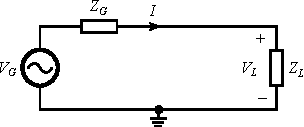
\includegraphics{img/analysis/generator_load}
    \caption{Equivalent circuit of a generator with given output impedance, $Z_G$, delivering power to a load of a given impedance, $Z_L$.}
    \label{fig:generator_load}
\end{figure}

To maximize the power transfered from a generator to a load, it is desired to have a reflection coefficient that is zero so that only forward waves are present on the transmission line. Figure~\ref{fig:generator_load} shows an equivalent circuit for this situation. The power in the load is found as \cite{pozar2011microwave}
\begin{equation}
    \label{eq:power1}
    P = \frac{1}{2} \real{V_LI^*} = \frac{1}{2} \real{\frac{|V_L|^2}{Z_L}}
    = \frac{1}{2} |V_L|^2 \real{\frac{1}{Z_L}}
\end{equation}
where
\begin{where}
\item[$P_L$] Power delivered to the load
\item[$V_L$] Voltage drop across the load
\item[$Z_L$] $R_L+jX_L$ is the load impedance
\item[$I$] Current through the load
\end{where}
Using basic circuit theory, (\ref{eq:power1}) can be expressed in terms of $V_G$ and $Z_G$, making it possible to derive the optimal $Z_G = R_G+jX_G$ for a fixed, complex load. Continuing from (\ref{eq:power1}),
\begin{equation}
    \begin{aligned}
        P &= \frac{1}{2} \left| V_G \frac{Z_L}{Z_L+Z_G} \right|^2 \real{\frac{1}{Z_L}} \\
        &= \frac{1}{2} |V_G|^2 \frac{|Z_L|^2}{|Z_L+Z_G|^2} \real{\frac{1}{Z_L}}\\
        &= \frac{|V_G|^2}{2} \frac{R_L^2+X_L^2}{(R_L+R_G)^2+(X_L+X_G)^2} \frac{R_L}{R_L^2 + X_L^2}\\
        &= \frac{|V_G|^2}{2} \frac{R_L}{(R_L+R_G)^2 + (X_L+X_G)^2}
    \end{aligned}
\end{equation}
The values of $R_G$ and $X_G$ that maximize the power delivered to the load, is found by 
\begin{enumerate}
\item Taking the partial derivative of $P$ with respect to $R_L$
\item Taking the partial derivative of $P$ with respect to $X_L$
\item Setting both of the above solutions equal to zero and solving for $R_G$ and $X_G$ (two equations with two unknowns)
    \begin{align}
        \dpd{P}{R_L} &= 0 \\
        \dpd{P}{X_L} &= 0
    \end{align}
\end{enumerate}
Doing so, yields the following solution,
\begin{equation}
    \begin{aligned}
        R_{G,\text{max}} &= R_L \\
        X_{G,\text{max}} &= -X_L
    \end{aligned}
\end{equation}
or $Z_{G,\text{max}} = Z^*_L$; the maximum power is transfered to the load when the generator impedance is the complex conjugate of the load impedance. In this situation the generator is said to be \emph{matched} to the load. Generally, the generator and the load would be connected through a transmission line with the characteristic impedance $Z_0$, so the maximum power transfer from generator to load will occur when both generator and load are matched to $Z_0$. 

% Mismatch loss, S11. |S11| = -6 dB  -->  SWR = 3
\begin{figure}[htbp]
    \centering
    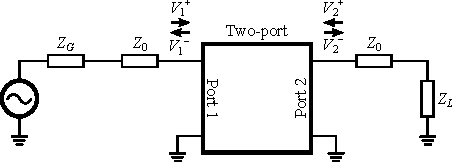
\includegraphics{img/analysis/s_parameter_twoport}
    \caption{S-parameters of a two-port system.}
    \label{fig:twoport}
\end{figure}

The reflection coefficient, $\Gamma$, can more generally be described as an \emph{S-parameter}. The S-parameters describe the ratio between the reflected and incident wave at a given port in a system. Consider a two-port as shown in Figure~\ref{fig:twoport}. Its four S-parameters are defined as follows:
\begin{align*}
    &S_{11} = \frac{V_1^-}{V_1^+} \Bigg|_{V_2^+=0} = \Gamma_1
    &&S_{12} = \frac{V_1^-}{V_2^+} \Bigg|_{V_1^+=0} \\
    &S_{21} = \frac{V_2^-}{V_1^+} \Bigg|_{V_2^+=0}
    &&S_{22} = \frac{V_2^-}{V_2^+} \Bigg|_{V_1^+=0} = \Gamma_2
\end{align*}
It is seen that $S_{11}$ and $S_{22}$ indicate the reflection due to the incident wave on the same port, when no contribution is made from the opposite port, i.e., these are the reflection coefficients of port 1 and 2, respectively. The parameter $S_{21}$ indicates how much of the incident wave on port 1 is coming out of port 2 when no wave is incident on port 2, i.e., this indicates the \emph{transmission coefficient} from port 1 to port 2. Likewise, $S_{12}$ is the transmission coefficient from port 2 to port 1.

The S-parameters are easily measured using a Vector Network Analyzer (VNA). The advantage of measuring S-parameters over, e.g., Y-parameters is that all ports are matched during the measurement instead of some being shorted, making odd behavior (like oscillations) less likely \cite{Bowick2007}.

% Smith chart visualization
\begin{figure}[htbp]
    \centering
    \begin{tikzpicture}
        \begin{smithchart}[mark repeat=3]
            \addplot coordinates {
                (0.5,0.2) 
                (0.5,0.3)
                (0.5,0.4)
                (0.5,0.5)
            };
            \path[draw=black, very thick] (0pt,0pt) circle (14.3mm);
        \end{smithchart}
    \end{tikzpicture}
    \caption{Smithchart. The circle illustrates the limit for which all points within the circle have a reflection coefficient below $\Gamma=0.5$ (or \SI{-6}{dB}). Two points -- $0.5+j0.2$ and $0.5+j0.5$ -- are shown.}
    \label{fig:smithchart}
\end{figure}
An important tool when doing matching, and designing antennas, to a certain $Z_0$ is the smith chart. The smith chart is used for plotting complex, normalized impedances and makes it easy to visually analyze the performance of a matched circuit. A smith chart is shown in Figure~\ref{fig:smithchart}.

The smith chart maps the entire right complex half-plane into a circle, having $0+j0$ all the way to the left and $\infty+j0$ all the way to the right. The y-axis (crossing $x=0$) makes up the circumference of the circle. An impedance is plotted by first finding the resistive (real) part of the impedance on the horizontal line and then following the circular grid-lines up or down for positive or negative reactances, respectively. 
The smith chart shown in Figure~\ref{fig:smithchart} is a normalized smith chart. When matching to $Z_0$, any impedance, $Z$, plotted in the smith chart, must be normalized by $Z_0$:
\begin{equation}
    Z_n = \frac{Z}{Z_0}
\end{equation}
This means that $Z_0$ will always appear at $1+j0$ -- in the center of the smith chart -- and the goal of the matching is to get the impedance of the antenna (or other circuitry) as close to the center as possible for the desired frequency range.

The impedance bandwidth of an antenna is often given as the bandwidth for which the reflection coefficient, $\Gamma$, is below 0.5 (or \SI{-6}{dB}). It may therefore be advantageous to plot this requirement. In the smith chart, this is plotted as a circle around the center and any point within the circle, is within the bandwidth of the circuit. The \SI{-6}{dB} circle is also shown in Figure~\ref{fig:smithchart}.

% Matching circuitry, L-network, smith chart ``ups and downs'', analytical formulas.
\begin{figure}[htbp]
    \begin{subfigure}{0.49\linewidth}
        \centering
        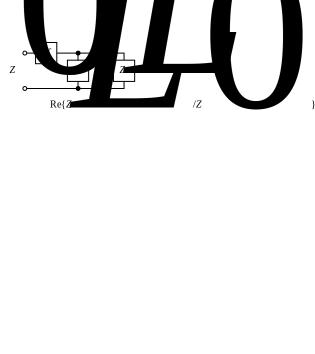
\includegraphics{img/analysis/l_network_a}
        \caption{Real part of normalized load impedance greater than one.}
        \label{fig:l_network_a}
    \end{subfigure}
    \hfill
    \begin{subfigure}{0.49\linewidth}
        \centering
        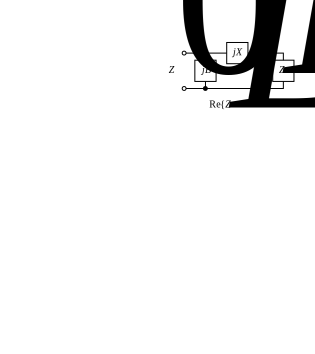
\includegraphics{img/analysis/l_network_b}
        \caption{Real part of normalized load impedance less than one.}
        \label{fig:l_network_b}
    \end{subfigure}
    \caption{L-network. The series/shunt configuration depends on the value of the load impedance.}
    \label{fig:l_network}
\end{figure}
In case the antenna is not designed to resonate exactly at the desired frequency or to the exact impedance bandwidth required, a tuning network can be placed immediately before the antenna. 

The simplest matching network is the L-network which is made from two components -- one in series an one in shunt -- as shown in Figure~\ref{fig:l_network}. The values of $X$ and $B$ correspond to the reactance of the chosen component at the frequency of interest. The equations of the network are shown below and the values of $X$ and $B$ are derived for both networks.

\fixme{Derive the equations below -- or just copy them from Pozar.}
\paragraph{For Figure~\ref{fig:l_network_a}}
The equations are as follows
\begin{align*}
    Z_0 = 
\end{align*}

\paragraph{For Figure~\ref{fig:l_network_b}}
\begin{align*}
    Z_0 = 
\end{align*}

\begin{itemize}
\item $X < 0$: Capacitor
\item $X > 0$: Inductor
\item $B < 0$: Inductor
\item $B > 0$: Capacitor
\end{itemize}



% Tuners: Series capacitor, shunt capacitor, variable inductor?

% Insertion loss, S21 for networks, equivalent series resistance, component Q.

\section{LTE}
In this part an overview of the allocated LTE frequency bands will be provided together with a general description of the lte spectrum.
Furthermore in addition to the allocated LTE bands a more detailed description on the bands covered in this project will be provided.

LTE (Long Term Evolution) is an evolution of the UMTS (Universal Mobile Telecommunications System), HSPA (High Speed Packet Access) and HSPA+ (Evolved High Speed Packet Access) 3G communication standards. HSPA and HSPA+ are upgrades to UMTS with the primary goal to improve the data rates on the 3G communication network. The LTE standard is marketed as a 4G network, even though the LTE standard do not meet the requirements set by the 4G standard.
The LTE provides much higher data rates than the 3G HSPA+ standard, using OFDMA (Orthogonal Frequency Division Multiplex) in downlink and SC-FDMA (Single Carrier - Frequency Division Multiple Access) in uplink. These access scheme technologies also enables the LTE network to use MIMO (Multiple Input Multiple Output) technologies, which has become a requirement in the in mobile phones.
MIMO technologies improves the throughput even further, by having the option to add up multipath signals. An comparison of the UMTS, HSPA and LTE speeds can be seen in table \ref{tab:3g4g_speeds}. \cite{radio2015electronics} 

\begin{table}[]
  \centering
  \begin{tabular}{|c|c|c|c|c|}
    \hline
    & {\bf \begin{tabular}[c]{@{}c@{}}WCDMA\\ (UMTS)\end{tabular}} & {\bf \begin{tabular}[c]{@{}c@{}}HSPA\\ HSDPA/HSUPA\end{tabular}} 
    & {\bf HSPA+} & {\bf LTE}     \\ \hline
    {\bf \begin{tabular}[c]{@{}c@{}}Max downlink speed\\ (bps)\end{tabular}} & 384 k & 14 M & 28 M & 100 M \\ \hline
    {\bf \begin{tabular}[c]{@{}c@{}}Max uplink speed\\ (bps)\end{tabular}} & 128 k & 5.7 M & 11 M & 50 M \\ \hline
    {\bf \begin{tabular}[c]{@{}c@{}}Latency\\ round trip time\\ approx\end{tabular}} & 150 ms & 100 ms & 50 ms (max) & ~10 ms \\ \hline
    {\bf Access methodology} & CDMA & CDMA & CDMA & OFDMA/SC-FDMA \\ \hline
  \end{tabular}
  \caption{LTE speed specifications \cite{radio2015electronics}}
  \label{tab:3g4g_speeds}
\end{table}

\subsection{LTE Frequency Band Allocation}
As seen in table \ref{tab:ltefreqband} the available LTE bands for uplink and downlink are allocated in the frequencies from \SIrange{452.5}{3600}{MHz}. The whole spectrum between \SIrange{452.5}{3600}{MHz} is not occupied by the mobile communication systems, as other network systems as WIFI, GPS and TV etc. also have the rights (licenses) to some of the frequency bands within this spectrum.
However the transition from analog to digital broadcast television signals, have freed some frequency bands for mobile communication. In U.S 2009 the \SI{700}{MHz} band covering \SIrange{698}{806}{MHz} was auctioned and latest the spectrum around \SI{600}{MHz} has also been freed and are put on auction this year \cite{Samantha2015tunableAntennas}. Furthermore in 2013 the \SI{800}{MHz} band, which also were freed due to the digital TV transition and the \SI{2600}{MHz} band was auctioned off by Ofcom \cite{james2014lte}.   

As the mobile communication is evolving now towards the 4'th generation, the need for higher data rates also increases, which leads to a need for more bandwidth. The freed bands increases the mobile communication spectrum both in the low and high frequencies, which can be used for different environments.  

\subsubsection{High and Low Frequency Bands}
The high and low frequency bands both have advantages and disadvantages. As seen in bands table \ref{tab:ltefreqband}, the band spacing varies form \SIrange{5}{90}{MHz}, the high frequencies providing high band spacing and the low frequencies low band spacing. This means that the high band frequencies provide greater capacity. One of the primary advantages of low band frequencies is the large wavelength. The large wavelength makes the waves able to travel long distances and is suitable for rural areas. The greater capacity at the high band frequencies makes these bands ideal for communication in urban areas as cities or other dense areas.

\subsubsection{Multiband LTE}
Most countries use several frequency bands across the LTE spectrum, which implies that a multiband phone/antenna is needed.  
Furthermore until now it has not been possible to agree on the same LTE band allocations across the world, because of the the different regulatory positions in different countries. Also in some cases across the different countries, the LTE bands are overlapping, as a consequence of different frequency availability around the world, thus limiting the accessibility of all users to use the same frequencies. \cite{radio2015electronics}.  

\begin{table}[]
  \centering
  \begin{tabular}{|c|c|c|c|c|c|}
    \hline
    \begin{tabular}[c]{@{}c@{}}LTE\\ band\\ number\end{tabular}  & \begin{tabular}[c]{@{}c@{}}Uplink\\ (MHz)\end{tabular} & \begin{tabular}[c]{@{}c@{}}Downlink\\ (MHz)\end{tabular}         & \begin{tabular}[c]{@{}c@{}}Width\\ of\\ band \\ spacing \\ (MHz)\end{tabular} & \begin{tabular}[c]{@{}c@{}}Duplex\\ spacing\\ (MHz)\end{tabular} & \begin{tabular}[c]{@{}c@{}}Band \\ Gap\\ (MHz)\end{tabular} \\ \hline
<<<<<<< .mine
    1  & 1920 - 1980 & 2110 - 2170 & 60 & 190 & 130 \\ \hline
    2  & 1850 - 1910 & 1930 - 1990 & 60 & 80  & 20  \\ \hline
    3  & 1710 - 1785 & 1805 - 1880 & 75 & 95  & 20  \\ \hline
    4  & 1710 - 1755 & 2110 - 2155 & 45 & 400  & 355  \\ \hline
    5  & 824 - 849   & 869 - 894   & 25 & 45  & 20  \\ \hline
    6  & 830 - 840   & 875 - 885   & 10 & 35  & 25  \\ \hline
    7  & 2500 - 2570 & 2620 - 2690 & 70 & 12  & 50  \\ \hline
    8  & 880 - 915   & 925 - 960   & 35 & 45  & 10  \\ \hline
    9  & 1749.9 - 17 & 1844.9 - 18 & 35 & 95  & 60  \\ \hline
    10 & 1710 - 1770 & 2110 - 2170 & 60 & 400  & 340  \\ \hline
    11 & 1427.9 - 14 & 1475.9 - 15 & 20 & 48  & 28  \\ \hline
    12 & 698 - 716   & 728 - 746   & 18 & 30  & 12  \\ \hline
    13 & 777 - 787   & 746 - 756   & 10 & -3  & 41  \\ \hline
    14 & 788 - 798   & 758 - 768   & 10 & -3  & 40  \\ \hline
    15 & 1900 - 1920 & 2600 - 2620 & 20 & 700  & 680  \\ \hline
    16 & 2010 - 2025 & 2585 - 2600 & 15 & 575 & 560 \\ \hline
    17 & 704 - 716   & 734 - 746   & 12 & 30  & 18  \\ \hline
    18 & 815 - 830   & 860 - 875   & 15 & 45  & 30  \\ \hline
    19 & 830 - 845   & 875 - 890   & 15 & 45  & 30  \\ \hline
    20 & 832 - 862   & 791 - 821   & 30 & -4  & 71  \\ \hline
    21 & 1447.9 - 14 & 1495.5 - 15 & 15 & 48  & 33  \\ \hline
    22 & 3410 - 3500 & 3510 - 3600 & 90 & 100  & 10  \\ \hline
    23 & 2000 - 2020 & 2180 - 2200 & 20 & 180  & 160  \\ \hline
    24 & 1625.5 - 16 & 1525 - 1559 & 34 & -1  & 13  \\ \hline
    25 & 1850 - 1915 & 1930 - 1995 & 65 & 80  & 15  \\ \hline
    26 & 814 - 849   & 859 - 894   & 30/40 &     & 10  \\ \hline
    27 & 807 - 824   & 852 - 869   & 17 & 45  & 28  \\ \hline
    28 & 703 - 748   & 758 - 803   & 45 & 55  & 10  \\ \hline
    29 & n/a         & 717 - 728   & 11 &     &     \\ \hline
    30 & 2305 - 2315 & 2350 - 2360 & 10 & 45  & 35  \\ \hline
    31 & 452.5 - 457 & 462.5 - 467 & 5  & 10  & 5   \\ \hline
||||||| .r48
    1  & 1920 - 1980 & 2110 - 2170 & 60 & 190 & 130 \\ \hline
    2  & 1850 - 1910 & 1930 - 1990 & 60 & 80  & 20  \\ \hline
    3  & 1710 - 1785 & 1805 - 1880 & 75 & 95  & 20  \\ \hline
    4  & 1710 - 1755 & 2110 - 2155 & 45 & 40  & 35  \\ \hline
    5  & 824 - 849   & 869 - 894   & 25 & 45  & 20  \\ \hline
    6  & 830 - 840   & 875 - 885   & 10 & 35  & 25  \\ \hline
    7  & 2500 - 2570 & 2620 - 2690 & 70 & 12  & 50  \\ \hline
    8  & 880 - 915   & 925 - 960   & 35 & 45  & 10  \\ \hline
    9  & 1749.9 - 17 & 1844.9 - 18 & 35 & 95  & 60  \\ \hline
    10 & 1710 - 1770 & 2110 - 2170 & 60 & 40  & 34  \\ \hline
    11 & 1427.9 - 14 & 1475.9 - 15 & 20 & 48  & 28  \\ \hline
    12 & 698 - 716   & 728 - 746   & 18 & 30  & 12  \\ \hline
    13 & 777 - 787   & 746 - 756   & 10 & -3  & 41  \\ \hline
    14 & 788 - 798   & 758 - 768   & 10 & -3  & 40  \\ \hline
    15 & 1900 - 1920 & 2600 - 2620 & 20 & 70  & 68  \\ \hline
    16 & 2010 - 2025 & 2585 - 2600 & 15 & 575 & 560 \\ \hline
    17 & 704 - 716   & 734 - 746   & 12 & 30  & 18  \\ \hline
    18 & 815 - 830   & 860 - 875   & 15 & 45  & 30  \\ \hline
    19 & 830 - 845   & 875 - 890   & 15 & 45  & 30  \\ \hline
    20 & 832 - 862   & 791 - 821   & 30 & -4  & 71  \\ \hline
    21 & 1447.9 - 14 & 1495.5 - 15 & 15 & 48  & 33  \\ \hline
    22 & 3410 - 3500 & 3510 - 3600 & 90 & 10  & 10  \\ \hline
    23 & 2000 - 2020 & 2180 - 2200 & 20 & 18  & 16  \\ \hline
    24 & 1625.5 - 16 & 1525 - 1559 & 34 & -1  & 13  \\ \hline
    25 & 1850 - 1915 & 1930 - 1995 & 65 & 80  & 15  \\ \hline
    26 & 814 - 849   & 859 - 894   & 30 &     & 10  \\ \hline
    27 & 807 - 824   & 852 - 869   & 17 & 45  & 28  \\ \hline
    28 & 703 - 748   & 758 - 803   & 45 & 55  & 10  \\ \hline
    29 & n/a         & 717 - 728   & 11 &     &     \\ \hline
    30 & 2305 - 2315 & 2350 - 2360 & 10 & 45  & 35  \\ \hline
    31 & 452.5 - 457 & 462.5 - 467 & 5  & 10  & 5   \\ \hline
=======
    1  & 1920--1980 & 2110--2170 & 60 & $190$ & 130 \\ \hline
    2  & 1850--1910 & 1930--1990 & 60 & $80$  & 20  \\ \hline
    3  & 1710--1785 & 1805--1880 & 75 & $95$  & 20  \\ \hline
    4  & 1710--1755 & 2110--2155 & 45 & $40$  & 35  \\ \hline
    5  & 824--849   & 869--894   & 25 & $45$  & 20  \\ \hline
    6  & 830--840   & 875--885   & 10 & $35$  & 25  \\ \hline
    7  & 2500--2570 & 2620--2690 & 70 & $12$  & 50  \\ \hline
    8  & 880--915   & 925--960   & 35 & $45$  & 10  \\ \hline
    9  & 1749.9--17 & 1844.9--18 & 35 & $95$  & 60  \\ \hline
    10 & 1710--1770 & 2110--2170 & 60 & $40$  & 34  \\ \hline
    11 & 1427.9--14 & 1475.9--15 & 20 & $48$  & 28  \\ \hline
    12 & 698--716   & 728--746   & 18 & $30$  & 12  \\ \hline
    13 & 777--787   & 746--756   & 10 & $-3$  & 41  \\ \hline
    14 & 788--798   & 758--768   & 10 & $-3$  & 40  \\ \hline
    15 & 1900--1920 & 2600--2620 & 20 & $70$  & 68  \\ \hline
    16 & 2010--2025 & 2585--2600 & 15 & $575$ & 560 \\ \hline
    17 & 704--716   & 734--746   & 12 & $30$  & 18  \\ \hline
    18 & 815--830   & 860--875   & 15 & $45$  & 30  \\ \hline
    19 & 830--845   & 875--890   & 15 & $45$  & 30  \\ \hline
    20 & 832--862   & 791--821   & 30 & $-4$  &  71  \\ \hline
    21 & 1447.9--14 & 1495.5--15 & 15 & $48$  & 33  \\ \hline
    22 & 3410--3500 & 3510--3600 & 90 & $10$  & 10  \\ \hline
    23 & 2000--2020 & 2180--2200 & 20 & $18$  & 16  \\ \hline
    24 & 1625.5--16 & 1525--1559 & 34 & $-1$  & 13  \\ \hline
    25 & 1850--1915 & 1930--1995 & 65 & $80$  & 15  \\ \hline
    26 & 814--849   & 859--894   & 30 &       & 10  \\ \hline
    27 & 807--824   & 852--869   & 17 & $45$  & 28  \\ \hline
    28 & 703--748   & 758--803   & 45 & $55$  & 10  \\ \hline
    29 & n/a        & 717--728   & 11 &       & \\ \hline
    30 & 2305--2315 & 2350--2360 & 10 & $45$  & 35  \\ \hline
    31 & 452.5--457 & 462.5--467 & 5  & $10$  & 5   \\ \hline
>>>>>>> .r75
  \end{tabular}
  \caption{LTE frequency band allocation (only frequency division duplex) \cite{radio2015electronics}}
  \label{tab:ltefreqband}
\end{table}

\subsection{Covered Bands}
In this project the frequencies of interest are \SIrange{700}{960}{MHz}, \SIrange{1710}{2170}{MHz}, \SIrange{2300}{2400}{MHz} and \SIrange{2550}{2650}{MHz}. These frequencies covers most of the LTE bands as seen in table \ref{tab:ltefreqband}. The bandwidth within this frequency range reaches from \SIrange{10}{70}{MHz}. The main goal of this project, is for the MIMO antenna's to be frequency reconfigurable within the above mentioned frequency range. As mentioned in the \fixme{introduction? reference.} the antenna MIMO antenna design will be consisting of two antennas, one covering the low frequencies from \SIrange{700}{960}{MHz} and one covering the high frequencies from \SIrange{1710}{2650}{MHz}. The antennas should be able to cover the highest bandwidth within these frequency spectrum's, which includes the downlink and uplink bandwidth and the duplex spacing bandwidth. For the low and high band antenna's to cover this bandwidth the low band antenna must be able to cover \SI{100}{MHz} and for the high band \SI{190}{MHz}.  


\section{User Effects}
\label{se:user_effects}
In this section the user impact on mobile antenna performance will be described, including both effects of the head, hand and the body in general.


Antenna parameters such as efficiency, radiation pattern, impedance etc. will be effected by the user, as the body of the user will look like a lossy and large dielectric body from the antennas point of view. 
The internal antennas that are implemented in every phone today, have a similar performance compared to external stubby antennas, which were used in a numerous of older designs. However this is only if the antennas are measured and compared in free space or next to a phantom head. In practical use a mobile phone with an internal antenna design, will be much more vulnerable to head and hand impacts from the user. The negative performance impact will be there, but will differ from user to user, as things like head and hand size, characteristics, hold position, left or right hand etc. varies from different users. This is of course a drawback in switching from external to internal antennas, but the development also comes with a lot of advantages. The internal antenna provides robust design and normally has higher performance in mechanical tests, such as drop tests, wearing tests etc. as the antenna is placed inside the phone, thus making physical interaction impossible. 
To counteract and minimize the user effect problem to the internal antennas, some basic design guidelines can be followed.

\subsection{Design Guidelines}
An antenna that is placed in the top of the phone, will be more effected by the user in talk mode, as the antenna will be closer to the head. To avoide this a ground plane can be placed between the user and the head in order to create more isolation. However placing the antenna on top of the ground plane decreases the bandwidth significantly, which leads to a, increase in the antenna size to keep the required bandwidth. This is not a reliable solution in mobile phones, as the size requirement of the antennas are very strict as a result of recent phone designs, with bigger screens and smaller cases. A way to solve this problem is to place the antenna in the bottom of the antenna, thus lowering the user effect and makes is possible to place the antenna without the ground plane as isolation. This solution provides a certain ground clearence, which makes it possible to decrease the volume and thickness of the antenna, thus saving place in the mobile phone. 
This design was proven to work by Motorola with there Motorola Razor V3 phone, which was the first phone to use the bottom placed antenna. There were some skeptics to this design, as the bottom of the phone would be placed in the middle of the hand in talk mode. However Motorola proved that theory wrong and therefore many phone manufactors are using there own bottom placed antennas. This solution of course only applies in talk mode, as the head effect is close to zero, when the phone is used in data mode. In data mode the phone is usually held either in horizontal mode with one hand or in vertical mode with two hands. In horizontal mode, given the size of today's smartphones, the hand will be placed around the middle of the phone, thus clearing the top and bottom. This indicates that it does not matter whether the antenna is placed in the top or bottom of the phone. In the case of horizontal mode with two hands, the hands covers both the top and the bottom of the phone, thus it still makes no difference if the antenna is placed in the bottom or in the top of the phone.

\begin{itemize}
\item Use tuning to compensate for the user effect (because of the changing impedans).
\end{itemize}

\subsection{Recent Measurements}
User effects of MIMO LTE performance 2014 measurements. \cite{Samantha2014UserEff}
\section{Frequency Division Time Domain}
\label{sec:fdtd}

\begin{itemize}
\item Conductivity what values to use, are they frequency dependent
\item permittivity what values to use, are they frequency dependent
\end{itemize}
\section{Problem Statement}
\label{sec:problem_statement}


% Requirements
\chapter{Requirements Specification}
\label{cha:reqspec}

\section{Functional Requirements}
\noindent
\begin{tabularx}{\linewidth}{|l|X|}
    \hline
    ID & Requirement \\
    \hline
    \freq{triband} & Two single-feed tri-band antennas covering. \\
    \freq{usereffect} & Must be able to re-tune any detuning due to user effects. \\
    \freq{matching} & Must have a simple matching network, containing a variable, shunt capacitor for tuning inside the specified bands.\\
    \freq{wispry} & Must use a wiSpry WS1040/WS1041 MEMS variable capacitor chip in the matching network.\\
    \hline
\end{tabularx}

\section{Specific Requirements}
\fixme{Update requirements}\\
\noindent 
\begin{tabularx}{\linewidth}{|l|X|X|}
    \hline
    ID & Specification & Requirement \\
    \hline
    \sreq{fbands} & Frequency bands\slash tunable range & \num{700}--\SI{960}{MHz}, \num{1710}--\SI{2170}{MHz}, \num{2300}--\SI{2400}{MHz}, \num{2550}--\SI{2650}{MHz} \\
    \sreq{physdim} & Physical dimensions & External: $70\times140\times7$\,\si{mm\cubed}, PCB: $55\times120$\,\si{mm\squared}\\
    \sreq{correlation} & Correlation between antenna elements & $\rho_e < 0.5$\\
    \sreq{efficiency} & Total efficiency of antenna (in-band) & $>\SI{50}{\%}$ \\
    \sreq{sar} & Maximum SAR & \\
    \sreq{insloss} & Maximum insertion loss & \\
    \hline
\end{tabularx}


% Testspecification
\chapter{Testspecification}
\subsubsection{Test of Requirement~\sreqref{fbands}---Frequency Bands/Tunable Range}
The frequency spectrum and the tunable range is tested by measuring the S11 and S22 parameters, using a VNA, for the top and side antenna respectively. The tunable range is done accordingly to requirement \sreqref{tunable} using a variable capacitor in the range \SI{0.3}{pF} to \SI{2.9}{pF} in steps of \SI{0.2}{pF} (\SI{0.1}{pF} minimum). 
\subsubsection{Test of Requirement~\sreqref{bandwidthlow}---Minimum Tunable Bandwidth in the Low Band}
The minimum required bandwidth in the low band  is measured as requirement~\sreqref{fbands}. The minimum required bandwidth is measured from the highest achievable bandwidth when sweeping each capacitor accordingly to requirement \sreqref{tunable}.

\subsubsection{Test of Requirement~\sreqref{bandwidthhigh}---Minimum Tunable Bandwidth in the High Band}
The minimum required bandwidth in the high band is measured as requirement~\sreqref{fbands}. The minimum required bandwidth is measured from the highest achievable bandwidth when sweeping each capacitor accordingly to requirement \sreqref{tunable}.

\subsubsection{Test of Requirement~\sreqref{bandwidthhigh}---Physical Dimensions}
The physical dimensions of the PCB, antenna and the external limitations are measured by a measuring tape. 

\subsubsection{Test of Requirement~\sreqref{copper}---Copper Thickness} This requirement is not tested, as the chosen PCB has a copper thickness of \SI{0.035}{mm}.

\subsubsection{Test of Requirement~\sreqref{correlation}---Correlation Between Antenna Elements}


\subsubsection{Test of Requirement~\sreqref{efficiency}---Total Efficiency in Free-Space}

\subsubsection{Test of Requirement~\sreqref{sar}---Maximum SAR}


\subsubsection{Test of Requirement~\sreqref{tunable}---Physical Dimensions} This requirement is not tested, as the variable capacitor chip is chosen as a wiSpry WS1040 MEMS chip accordingly to requirement~\freqref{wispry}. 

\cite{cita2015}

% Technical solution
\chapter{Technical Solution}
In this chapter, the technical solution will be documented. The technical solution includes three antenna designs simulated and measured in free-space and with user effects. All the antenna designs are done accordingly to the requirement specification, Chapter~\ref{cha:reqspec}. 

\section{Monopole Antenna}
\label{sec:techsol1_monopole}

\begin{figure}[htbp]
    \begin{subfigure}[b]{0.49\linewidth}
        \centering
        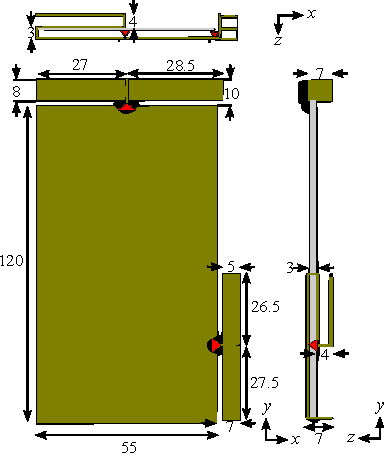
\includegraphics{img/tech_sol/monopole/tech_drawing}
        \caption{Technical drawing.}
        \label{fig:ant1technical}
    \end{subfigure}
    \hfill
    \begin{subfigure}[b]{0.49\linewidth}
        \centering
        \includegraphics{img/tech_sol/schematic_tuning_1}\\[1cm]
\footnotesize
        \begin{tabular}{|l|l|l|l|}
            \hline
            & $C_1$ & $L_1$ & $C_2$ \\
            \hline
            Top antenna & \SI{3.02}{pF} & \SI{7.99}{nH} & $[0.3,2.9]\,$pF\\
            Side antenna & \SI{1.81}{pF} & \SI{5.27}{nH} & $[0.3,2.9]\,$pF\\
            \hline
        \end{tabular}
        \caption{Tuning/matching circuit.}
    \end{subfigure}
    \caption{Technical drawing and tuning circuit for the antenna.  The matching circuit is applied for both the top and the side antenna.}
    \label{fig:ant1techschem}
\end{figure}

%Single antenna description
The antenna design, for both antennas, is shown in Figure~\ref{fig:ant1technical}. Both antennas are designed from a basic folded monopole structure with two arms -- one for the low band and one for the high band. The antennas are almost identical with a few changes as a result of the restrictions on the ground clearance.
The antennas are designed to take full advantage of the ground clearance requirements in both height, length, and width. This is done in order to obtain the highest possible bandwidth in both bands. 

%MIMO
Going from the top antenna to the side antenna, the ground clearance decreases from \SI{10}{mm} to \SI{7}{mm}. To compensate for the decrease in ground clearance the length of both the low band and high band arms are adjusted. This is done to obtain the highest bandwidth within the low band and high band. 

The surface currents of the top antenna are shown in Figure~\ref{fig:ant1_sc}. In the low band, the left arm is excited and, as the frequency increases, the short arm becomes more excited. This illustrates the different operation modes of the two arm folded monopole structure.

The $S$-parameter for both antennas can be seen in Figure~\ref{fig:ant1_sparam}. Both antennas are simulated with the tuning capacitors at \SI{0.3}{pF}. In this state, both antennas cover the highest frequencies in the low and the high band. From the figure, it can be seen that both antennas almost covers the entire high band. However, some tuning is needed for the side antenna in the lower band.

\begin{figure}[htbp]
   \begin{subfigure}[b]{0.32\linewidth}
        \centering
        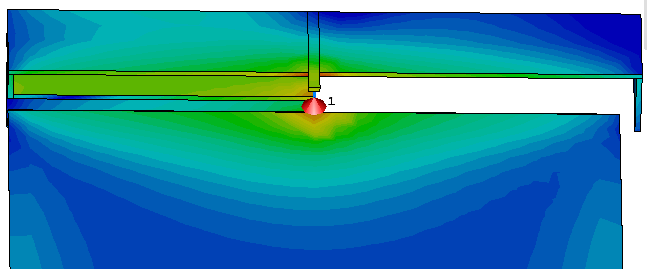
\includegraphics[width=\linewidth]{img/tech_sol/monopole/sc_800}
        \caption{Surface current for \SI{800}{MHz}}
        \label{fig:ant1_sc800}
    \end{subfigure}
    \hfill
    \begin{subfigure}[b]{0.32\linewidth}
        \centering
        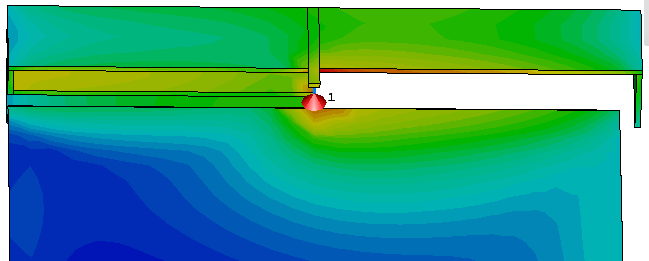
\includegraphics[width=\linewidth]{img/tech_sol/monopole/sc_1800}
        \caption{Surface current for \SI{1800}{MHz}}
        \label{fig:ant1_sc1800}
    \end{subfigure}
    \hfill
    \begin{subfigure}[b]{0.32\linewidth}
        \centering
        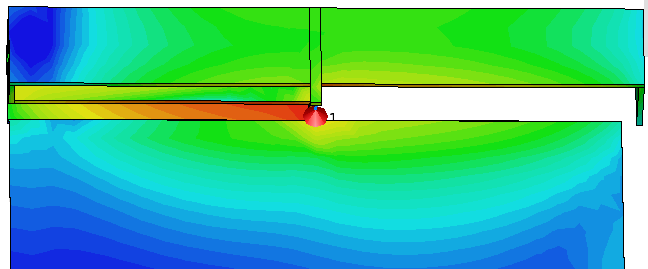
\includegraphics[width=\linewidth]{img/tech_sol/monopole/sc_2400}
        \caption{Surface current for \SI{2400}{MHz}}
        \label{fig:ant1_sc2400}
    \end{subfigure}
    \caption{Surface currents at each resonance with $C_2=\SI{0.3}{pF}$.}
    \label{fig:ant1_sc}
\end{figure}

\begin{figure}[htbp]
    \centering
    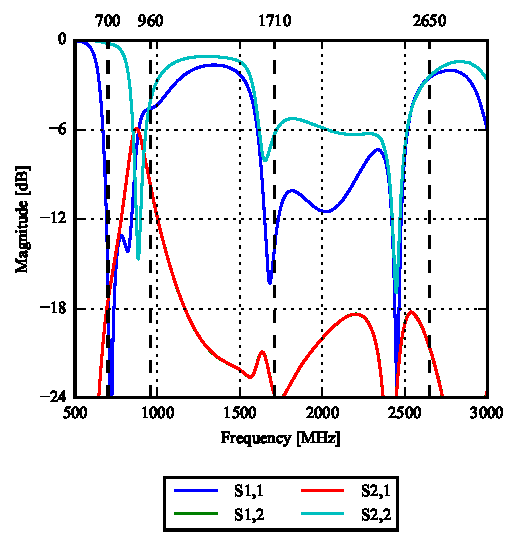
\includegraphics{img/tech_sol/monopole/ant1_sparam}
    \caption{S-parameters with $C_2=\SI{0.3}{pF}$ for both antennas.}
    \label{fig:ant1_sparam}
\end{figure}
%%
The tuned $S$-parameters for both antennas can be seen in Figure~\ref{fig:sparam_mono_free_space}. The return losses, $-S_{11}$ and $-S_{22}$, show that both antennas almost cover the desired bandwidth. However, from \SI{2500}{MHz} to \SI{2650}{MHz}, both antennas are \SI{1}{dB} to \SI{3}{dB} lower than required. The side antenna also shows a lower level than desired at \SI{1750}{MHz} and in the low band limits. During the $S$-parameter simulation sweep of one antenna, the variable capacitor of the other antenna is set to the initial fixed value of \SI{0.3}{pF}. 

%%
The isolation loss, $S_{21}$, is shown in Figure~\ref{fig:sparam_mono_free_space}. The $S_{21}$ sweep shows a low isolation loss at \SI{5}{dB} in the low band. The surface current simulations, shown in Figure~\ref{fig:ant1_sc}, show that the monopole antenna design excites the ground plane, which could cause the low isolation loss. This should be taken into consideration as the isolation loss can have a significant effect on the MIMO performance.

%%
The channel bandwidth for both antennas are shown in Table~\ref{tab:bw_sol1}. Both antennas fulfill the desired bandwidth requirement in the lower bands. However, only the top antenna complies with the bandwidth requirement in the high band where the side antenna lacks \SI{37}{MHz}.

%Correlation %%
The correlation, between the antennas, is shown in Figure~\ref{fig:corr_sol1}. The figure shows the correlation when sweeping the tuning capacitors from \SI{0.3}{pF} to \SI{2.9}{pF}. From the figure, it is seen that the correlation exceeds the requirement of \num{0.5} in the low band for both the top and side antenna with a maximum at \SI{700}{MHz}. The surface currents at the different operation frequencies, seen in Figure~\ref{fig:ant1_sc}, show a strong coupling to the ground plane, which could cause the high correlation in the low band.

%Efficiency %%
The efficiency for both antennas is shown in Figure~\ref{fig:eff_sol1_free}. The efficiency is plotted for each sweep of the tunable capacitors. The efficiency mostly covers the desired spectrum at an efficiency of \SI{-3}{dB} with a drop of \SI{1.5}{dB} around \SI{750}{MHz} for the side antenna. 

    \begin{table}
        \centering
        \begin{tabular}{|l|l|r|r|r|}
            \hline
            Antenna & Band & Start [MHz] & Stop [MHz] & Bandwidth [MHz] \\
            \hline
            Top     & Low  & 680         & 1011       & 331 \\
            Side    & Low  & 818         & 909        & 91 \\
            \hline
            Top     & High & 1590        & 2527       & 937 \\
            Side    & High & 1850        & 2533       & 683 \\
            \hline
        \end{tabular}
        \caption{Maximum bandwidth obtained in the low and high band for the top and the side antenna, respectively.}
        \label{tab:bw_sol1}
    \end{table}

%S-Parameter sweep
\begin{figure}[htbp]
   \begin{subfigure}[b]{0.49\linewidth}
        \centering
        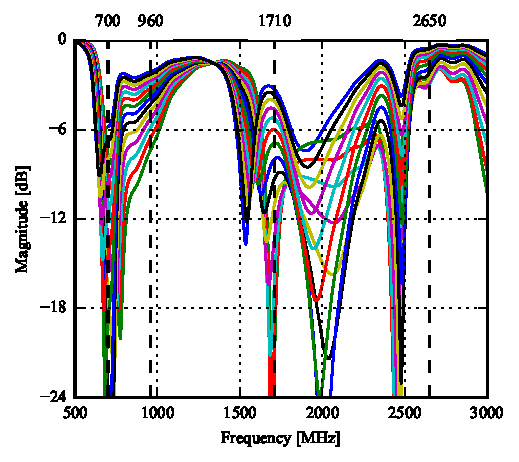
\includegraphics{img/tech_sol/monopole/s11}
        \caption{$S_{11}$, sweeping $C_1$ and fixing $C_2$.}
    \end{subfigure}
    \hfill
    \begin{subfigure}[b]{0.49\linewidth}
        \centering
        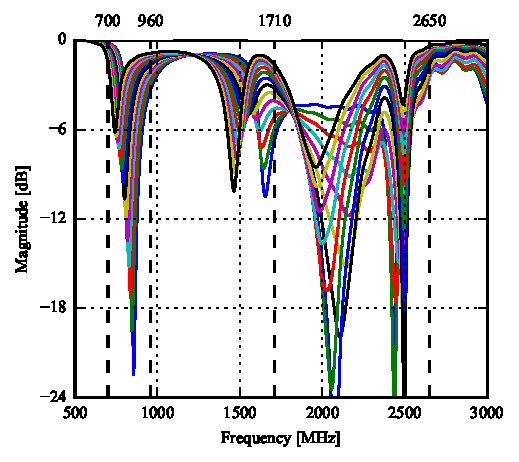
\includegraphics{img/tech_sol/monopole/s22}
        \caption{$S_{22}$, sweeping $C_2$ and fixing $C_1$.}
    \end{subfigure}
~
    \begin{subfigure}[b]{0.49\linewidth}
        \centering
        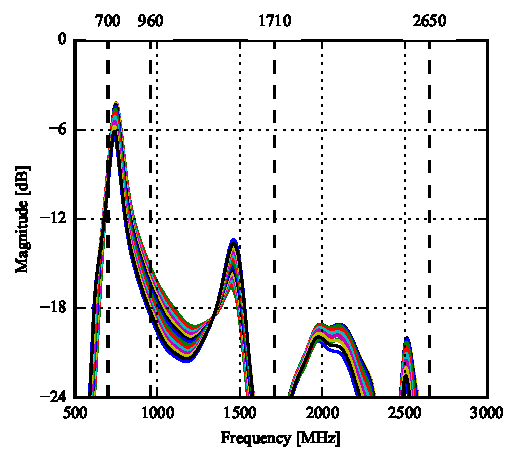
\includegraphics{img/tech_sol/monopole/s21-s11}
        \caption{$S_{21}$, sweeping $C_1$ and fixing $C_2$.}
    \end{subfigure}
    \hfill
    \begin{subfigure}[b]{0.49\linewidth}
        \centering
        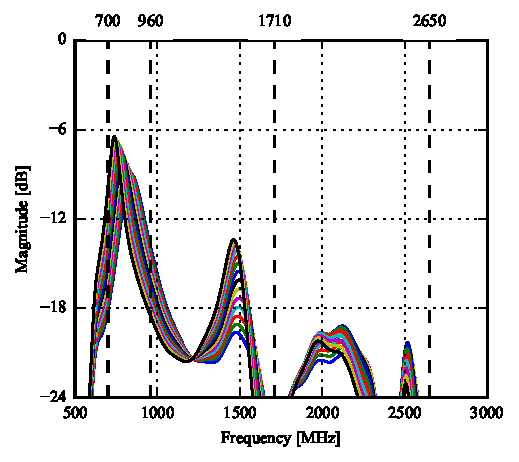
\includegraphics{img/tech_sol/monopole/s21-s22}
        \caption{$S_{21}$, sweeping $C_2$ and fixing $C_1$.}
    \end{subfigure}
    \caption{$S$-parameter sweep in free space for tuning the shunt capacitor of each antenna, $C_1$ and $C_2$ for port 1 and 2, respectively. Port 1 is the top antenna and port 2 is the side antenna.}
    \label{fig:sparam_mono_free_space}
\end{figure}

% Correlation
\begin{figure}[htbp]
    \centering
    \begin{subfigure}{0.49\linewidth}
        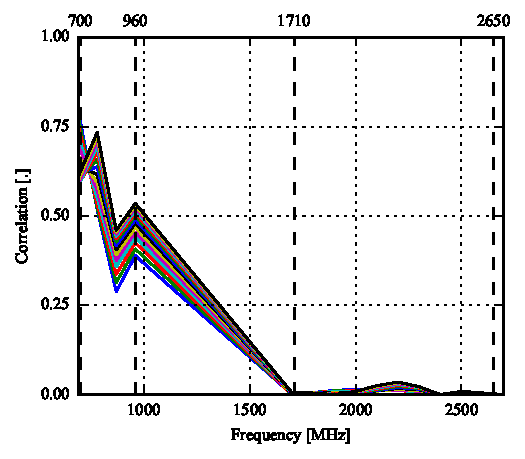
\includegraphics{img/tech_sol/monopole/free_space/s11_corr}
        \caption{Sweeping $C_1$ and fixing $C_2$.}
    \end{subfigure}
    \hfill
    \begin{subfigure}{0.49\linewidth}
        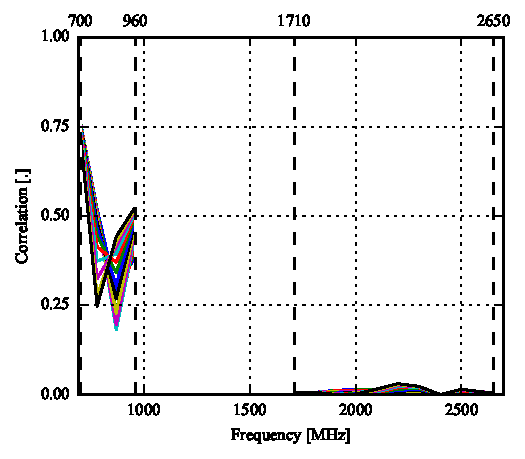
\includegraphics{img/tech_sol/monopole/free_space/s22_corr}
        \caption{Sweeping $C_2$ and fixing $C_1$.}
    \end{subfigure}
    \caption{Correlation between the antennas when sweeping tuning capacitors. Here, $C_1$ and $C_2$ are the tuning capacitor for the top and side antenna, respectively.}
    \label{fig:corr_sol1}
\end{figure}

\begin{figure}[htbp]
    \centering
    \begin{subfigure}{0.49\linewidth}
        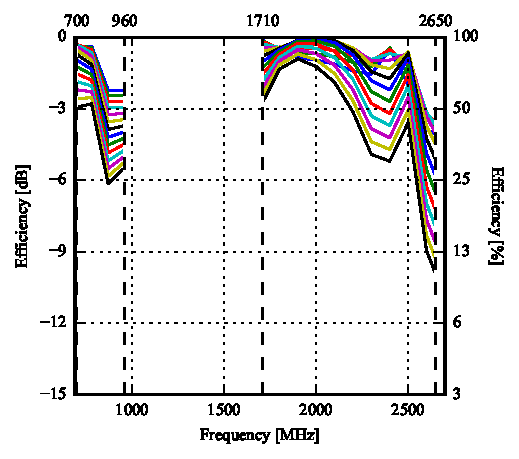
\includegraphics{img/tech_sol/monopole/free_space/efficiency-ac1-csh1}
        \caption{Sweeping $C_1$ and fixing $C_2$.}
    \end{subfigure}
    \hfill
    \begin{subfigure}{0.49\linewidth}
        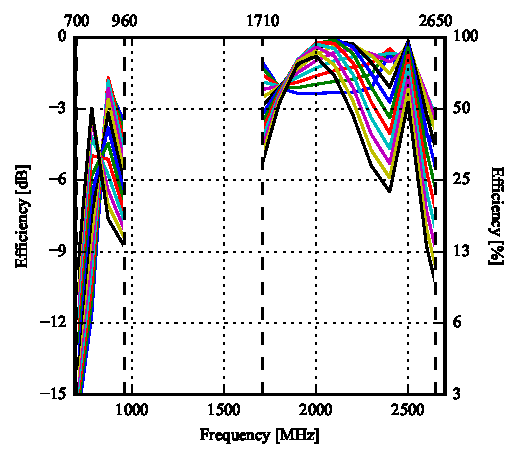
\includegraphics{img/tech_sol/monopole/free_space/efficiency-ac2-csh2}
        \caption{Sweeping $C_2$ and fixing $C_1$.}
    \end{subfigure}
    \caption{Efficiency for each antenna when sweeping the tunable capacitors. Here, $C_1$ and $C_2$ are the tuning capacitor for the top and side antenna, respectively.}
    \label{fig:eff_sol1_free}
\end{figure}

\section{Triangle-Feed Antenna}
\label{sec:techsol_triang}

\begin{figure}[htbp]
    \begin{subfigure}[b]{0.49\linewidth}
        \centering
        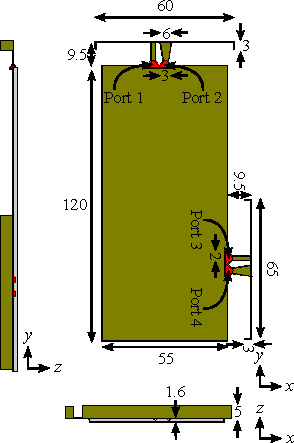
\includegraphics{img/tech_sol/trianglefeed/technical}
        \caption{Technical drawing. Unit: mm.}
        \label{fig:ant2technical}
    \end{subfigure}
    \hfill
    \begin{subfigure}[b]{0.49\linewidth}
        \centering
        \includegraphics{img/tech_sol/schematic_tuning_1}\\[1cm]
        \footnotesize
        \begin{tabular}{|l|l|l|l|}
            \hline
            & $C_1$ & $L_1$ & $C_2$ \\
            \hline
            Top antenna & \SI{3.45}{pF} & \SI{7.89}{nH} & $[0.3,2.9]\,$pF\\
            Side antenna & \SI{2.42}{pF} & \SI{5.69}{nH} & $[0.3,2.9]\,$pF\\
            \hline
        \end{tabular}
        \caption{Tuning/matching circuit.}
        \label{fig:ant2schematic}
    \end{subfigure}
    \caption{Technical drawing and tuning circuit for the antenna.  The antennas are built on FR-4 board using \SI{35}{\micro\meter} copper. There is a matching circuit as shown for each of the two feeds.}
    \label{fig:ant2techschem}
\end{figure}

The antenna is shown in Figure~\ref{fig:ant2techschem}. The two antennas each consist of a triangle-feed printed on FR-4 and the main element following the edge of this FR-4 block.

% What makes it radiate at 900, 1800, and 2400?
The low-band element consists of a CCE (Capacitively Coupled Element) antenna which is inherently non-resonant \cite{valkonen2013inherently,ilvonen2014design}. The resonance of this type of antenna is dependent on the matching circuit. For this design, the matching is performed by $C_1$ and $L_1$ to resonate at \SI{960}{MHz} and $C_2$ is used to tune the resonance frequency down to \SI{700}{MHz}.

The triangular feed creates two new resonances in the mid-band (around \SI{1800}{MHz}) and the high-band (around \SI{2400}{MHz}). Looking at the top-antenna, the right-hand side from the feed line resonates at around \SI{1800}{MHz} and the left-hand side resonates at around \SI{2400}{MHz}. By determining the $x$-position of the triangle-feed, these two resonances can either be separated or joined, making it possible to cover all the required high LTE bands. The surface currents, illustrating how the structure resonates after matching, is shown in Figure~\ref{fig:ant2surfaces}.

\begin{figure}[htbp]
    \centering
    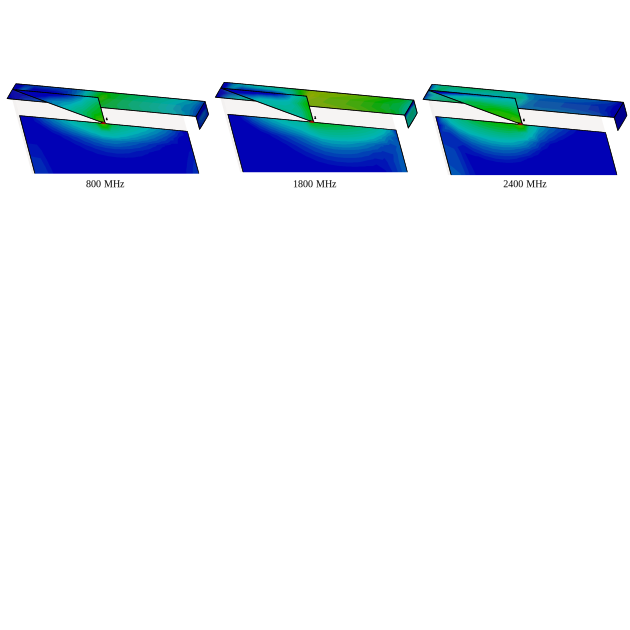
\includegraphics{img/tech_sol/trianglefeed/surface_currents}
    \caption{Surface currents around each resonance with $C_2=\SI{0.3}{pF}$.}
    \label{fig:ant2surfaces}
\end{figure}

\begin{figure}[htbp]
    \centering
    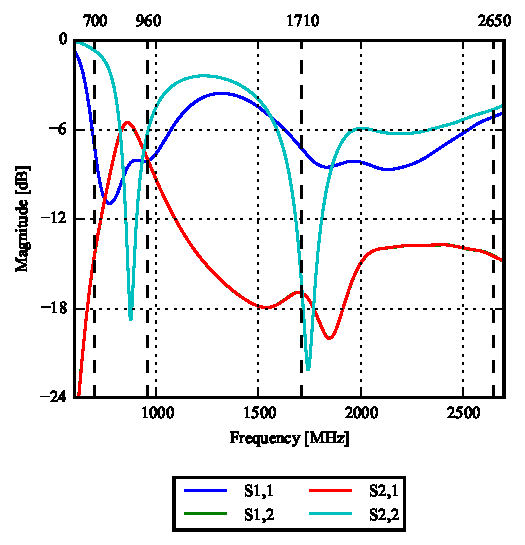
\includegraphics{img/tech_sol/trianglefeed/sparams}
    \caption{S-parameters with $C_2=\SI{0.3}{pF}$ for both antennas.}
    \label{fig:ant2sparams}
\end{figure}

%%
The $S$-parameters for both antennas are shown in Figure~\ref{fig:ant2sparams} with the tuning capacitors at their minimum values, \SI{0.3}{pF}. At this position, the highest end of the low band, around \SI{960}{MHz}, is covered. It is seen that the top-antenna (port 1) covers the whole lower band whereas the side-antenna only covers around half of the band and must be tuned to cover the whole band. The high band is almost covered at this capacitor setting for both antennas.

%%
The tuned $S$-parameters are shown in Figure~\ref{fig:ant2sweeps}. Here is seen that the entire lower band can be covered by the side antenna ($S_{22}$) and that the entire high band is covered at $C_2 = \SI{0.7}{pF}$ to \SI{0.9}{pF} for the top- and side-antenna respectively. It is noted that all three resonances are moved when $C_2$ is altered.

% Sweep description %%
It is seen that the isolation at low frequencies is only around \SI{5}{dB}. This may cause problems when using the antennas for MIMO operation. The bad isolation may be caused by the way the CCE antenna resonates. The CCE antenna couples to the chassis and uses this as a resonator \cite{ilvonen2014design}. This may cause high correlation when both antennas couple to the chassis.

This design provides high bandwidth, covering all desired bands for both antennas. However, the isolation between the two antennas is not the best. Additionally, building the antenna on lossy FR-4 may prove to decrease the efficiency bandwidth compared to an antenna with a less lossy isolator.

\begin{table}[htbp]
    \centering
    \begin{tabular}{|l|l|r|r|r|}
        \hline
        Antenna & Band & Start [MHz] & Stop [MHz] & Bandwidth [MHz] \\
        \hline
        Top     & Low  & 688         & 1073       & 385 \\
        Side    & Low  & 824         & 962        & 138 \\
        \hline
        Top     & High & 1577        & 2637       & 1060 \\
        Side    & High & 1535        & 2654       & 1119 \\
        \hline
    \end{tabular}
    \caption{Maximum bandwidth obtained in the low and high band for the top and the side antenna, respectively.}
    \label{tab:bw_sol2}
\end{table}

% Bandwidth %%
The bandwidth in the high and low band for each antenna is shown in Table~\ref{tab:bw_sol2}. It is clear that both antennas fulfill the requirements of tunable impedance bandwidth seen in the requirement specification, Section~\ref{cha:reqspec}.

\begin{figure}[htbp]
    \centering
    \begin{subfigure}{0.49\linewidth}
        \centering
        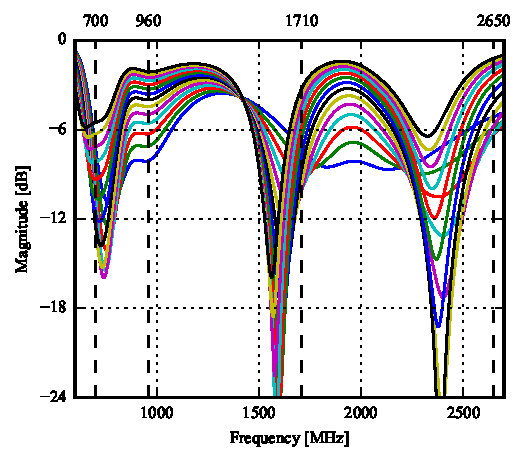
\includegraphics{img/tech_sol/trianglefeed/Csh1s11.pdf}
        \caption{$S_{11}$, sweeping $C_1$ and fixing $C_2$.}
    \end{subfigure}
    \hfill
    \begin{subfigure}{0.49\linewidth}
        \centering
        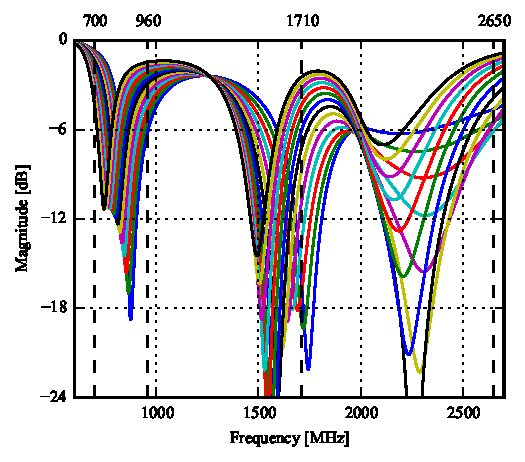
\includegraphics{img/tech_sol/trianglefeed/Csh2s22.pdf}
        \caption{$S_{22}$, sweeping $C_2$ and fixing $C_1$.}
    \end{subfigure}
    \vspace*{1em}
    \begin{subfigure}{0.49\linewidth}
        \centering
        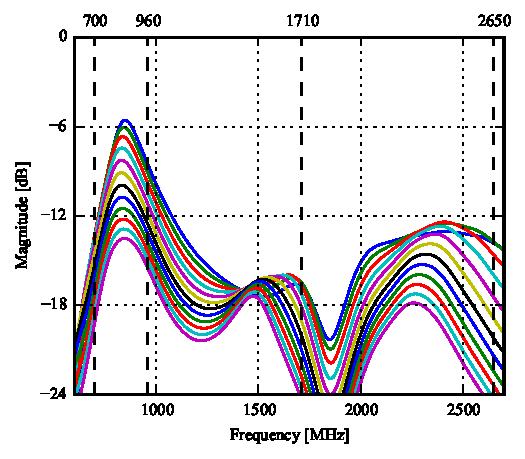
\includegraphics{img/tech_sol/trianglefeed/Csh1s21.pdf}
        \caption{$S_{21}$, sweeping $C_1$ and fixing $C_2$.}
    \end{subfigure}
    \hfill
    \begin{subfigure}{0.49\linewidth}
        \centering
        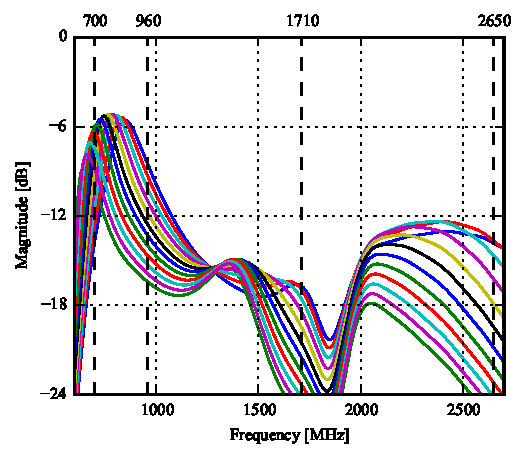
\includegraphics{img/tech_sol/trianglefeed/Csh2s21.pdf}
        \caption{$S_{21}$, sweeping $C_2$ and fixing $C_1$.}
    \end{subfigure}
    \caption{Parameter sweeps when tuning the shunt capacitor of each antenna, $C_{1}$ and $C_{2}$ for port 1 and 2, respectively. Port 1 is the top antenna and port 2 is the side antenna.}
    \label{fig:ant2sweeps}
\end{figure}

% Correlation
\begin{figure}[htbp]
    \centering
    \begin{subfigure}{0.49\linewidth}
        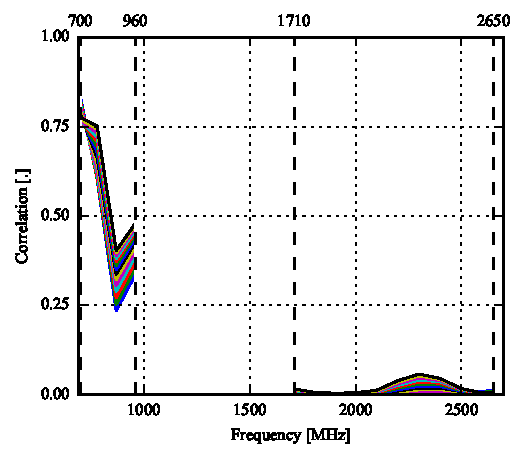
\includegraphics{img/tech_sol/trianglefeed/corr/correlation_Csh1-sweep}
        \caption{Sweeping $C_1$ and fixing $C_2$.}
    \end{subfigure}
    \hfill
    \begin{subfigure}{0.49\linewidth}
        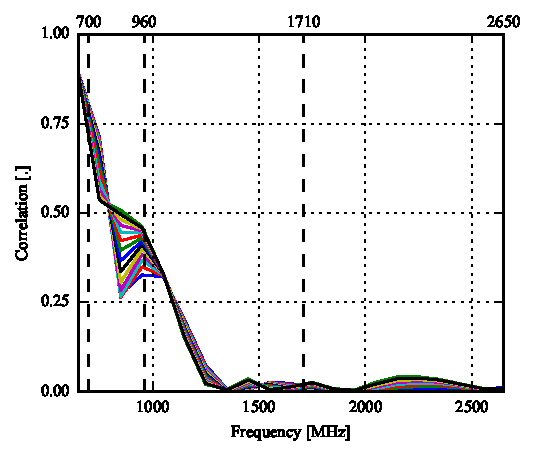
\includegraphics{img/tech_sol/trianglefeed/corr/correlation_Csh2-sweep}
        \caption{Sweeping $C_2$ and fixing $C_1$.}
    \end{subfigure}
    \caption{Correlation between the antennas then sweeping tuning capacitors. Here, $C_1$ and $C_2$ are the tuning capacitor for the top and side antenna, respectively.}
    \label{fig:corr_sol2}
\end{figure}

%%
The correlation between the top an side antennas are shown in Figure~\ref{fig:corr_sol2} when sweeping the tuning capacitors. It is seen that the correlation in the high band is very low while the correlation in the low band is not the best. This may be caused by the fact that both antennas are coupling to the ground plane to radiate. A solution might be to use a different type of antenna design for the side.

% Efficiency
\begin{figure}[htbp]
    \centering
    \begin{subfigure}{0.49\linewidth}
        \centering
        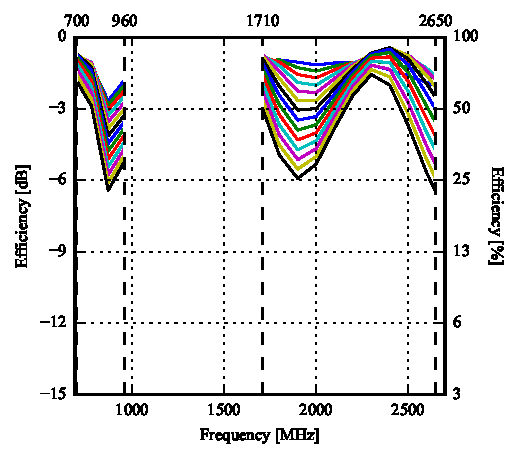
\includegraphics{img/tech_sol/trianglefeed/efficiency-ac1-csh1.pdf}
        \caption{Top antenna. Sweeping $C_1$, fixing $C_2$.}
    \end{subfigure}
    \hfill
    \begin{subfigure}{0.49\linewidth}
        \centering
        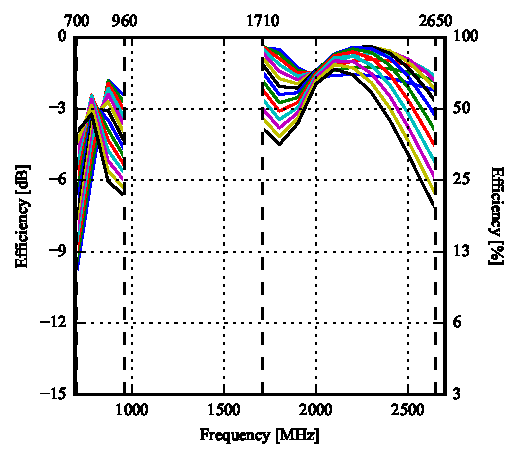
\includegraphics{img/tech_sol/trianglefeed/efficiency-ac2-csh2.pdf}
        \caption{Side antenna. Sweeping $C_2$, fixing $C_1$.}
    \end{subfigure}
    \caption{Efficiency for each antenna when sweeping the tuning capacitors. Here, $C_1$ and $C_2$ are the tuning capacitor for the top and side antenna, respectively.}
    \label{fig:eff_sol2}
\end{figure}

%%
The total system efficiency (i.e.\ including mismatch loss) is shown for a sweep of capacitance values in Figure~\ref{fig:eff_sol2}. It is seen that, for the lowest capacitance setting, the top antenna has a total efficiency greater than \SI{-3}{dB}. The side antenna has a total efficiency greater than \SI{-3}{dB} in the high band for its low capacitance settings. In the low band, the antenna can be tuned to cover the whole band at a total efficiency above \SI{-4}{dB}.

\section{Antenna Design 3 - Broken Arrow}


\chapter{User Effect Simulations}
\label{cha:usereff}
In this chapter, the antennas from Chapter~\ref{cha:nousersim} are simulated in use.
The four simulation models are shown in Figure~\ref{fig:usereff_intro}. The SAR simulation is solely used to check the requirement for maximum SAR seen in the requirement specification, Chapter~\ref{cha:reqspec}. For the other three simulations, the same results as in Chapter~\ref{cha:nousersim} are shown to see how the antennas perform when the phones are in use.

All the simulations are done with a phone case in order to align the phone and make the simulations more accurate. The case used is made of thin \SI{0.5}{mm} plastic and is customized to fit each antenna design. Furthermore to make the SAR simulations even more accurate a screen model made of PEC is used.  

The below settings were used when simulating the user effect:
\begin{description}
\item[Accuracy] \SI{-60}{dB}.
\item[One hand (data mode)] Approximately \num{7500000} mesh cells.
\item[Two hands (play mode)] Approximately \num{15000000} mesh cells.
\item[Head and hand (talk mode, SAR)] Approximately \num{15000000} mesh cells.
\end{description}

The material types and constants can be seen in Table \ref{tab:cst_material}. The head, hand and spacer is made accordingly to the CTIA test plan \cite{cita2015}. Second order permittivity dispersion model fits have been used for the head and hand models to gain more accurate results in the user effect simulations.

\begin{table}
  \centering
  \begin{tabular}{|l|l|r|r|}
    \hline
    Type & Material & Permeability [$\mu$] & Permittivity [$\epsilon$] \\
    \hline
    Case      & Plastic  & 1    & 3       \\
    Spacer    & Vacuum   & 1    & 1       \\
    Hand      & Shell and fluid   & 1    & 2nd order disp.     \\
    Head      & Shell    & 1    & 3.7     \\
    Head      & Fluid    & 1    & 2nd order disp.     \\ 
    \hline
  \end{tabular}
  \caption{Material types and constants used in the user effect simulations.}
  \label{tab:cst_material}
\end{table}

\begin{figure}[htbp]
  \centering
  \begin{subfigure}[b]{0.24\linewidth}
        \centering
        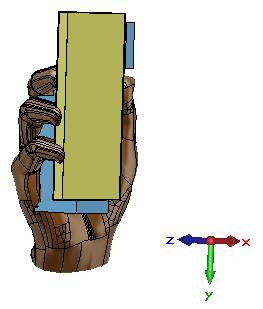
\includegraphics[width=\linewidth, height=4cm, keepaspectratio]{img/tech_sol/usereff_intro/usereff_onehand}
        \caption{Data mode.}
        \label{fig:usereff_onehand}
    \end{subfigure}
    \hfill
    \begin{subfigure}[b]{0.24\linewidth}
        \centering
        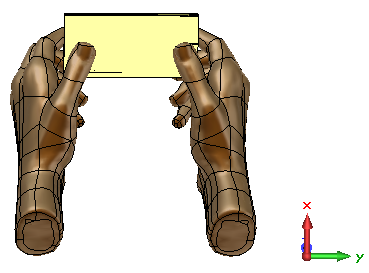
\includegraphics[width=\linewidth, height=4cm, keepaspectratio]{img/tech_sol/usereff_intro/usereff_twohand}
        \caption{Play mode.}
        \label{fig:usereff_twohand}
    \end{subfigure}
    \hfill
    \begin{subfigure}[b]{0.24\linewidth}
        \centering
        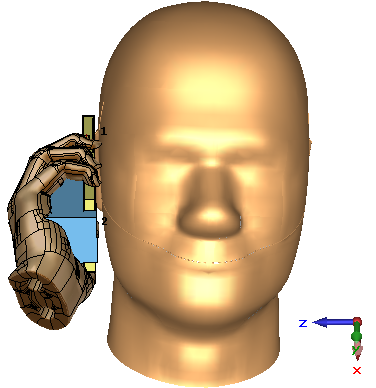
\includegraphics[width=\linewidth, height=4cm, keepaspectratio]{img/tech_sol/usereff_intro/usereff_headhand}
        \caption{Talk mode.}
        \label{fig:usereff_headhand}
    \end{subfigure}
    \hfill
    \begin{subfigure}[b]{0.24\linewidth}
        \centering
        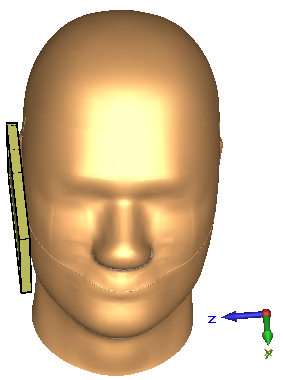
\includegraphics[width=\linewidth, height=4cm, keepaspectratio]{img/tech_sol/usereff_intro/usereff_sar}
        \caption{SAR simulation.}
        \label{fig:usereff_sar}
    \end{subfigure}
    \caption{User effect simulation modes.}
    \label{fig:usereff_intro}
\end{figure}

\section{Antenna Design 1 -- Monopole}
In this section, the antenna from Section~\ref{sec:techsol1_monopole} will be simulated in pratice use with an user. The antenna positions are shown in Figure~\ref{fig:sol1_monoant_positions}.

\begin{figure}[htbp]
    \centering
    \begin{subfigure}[b]{0.24\linewidth}
        \centering 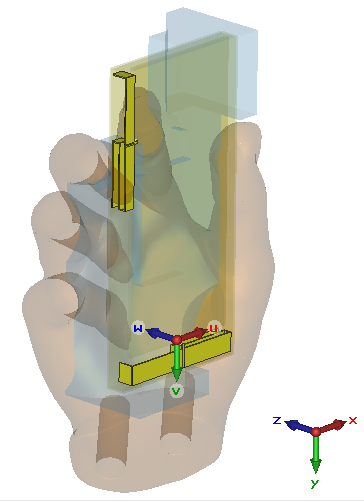
\includegraphics[width=\linewidth,height=4cm,keepaspectratio]{img/tech_sol/monopole/data_mode/3d_data_mode.PNG}
        \caption{Data mode.}
    \end{subfigure}
    \begin{subfigure}[b]{0.24\linewidth}
        \centering 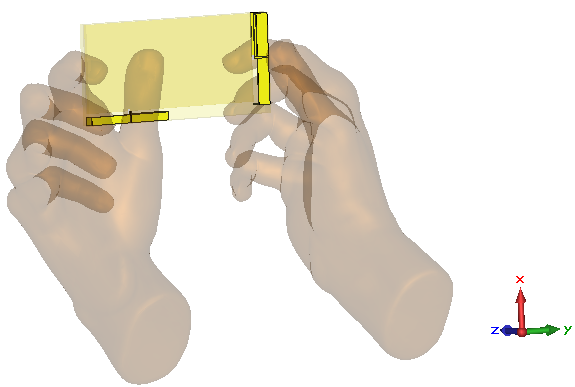
\includegraphics[width=\linewidth,height=4cm,keepaspectratio]{img/tech_sol/monopole/play_mode/3d_play_mode.PNG}
        \caption{Play mode.}
    \end{subfigure}
    \begin{subfigure}[b]{0.24\linewidth}
        \centering 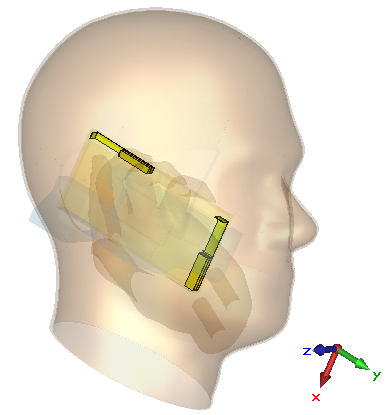
\includegraphics[width=\linewidth,height=4cm,keepaspectratio]{img/tech_sol/monopole/talk_mode/3d_talk_mode.PNG}
        \caption{Talk mode.}
    \end{subfigure}
    \begin{subfigure}[b]{0.24\linewidth}
        \centering \includegraphics[width=\linewidth,height=4cm,keepaspectratio]{img/tech_sol/monopole/sar/3d_sar.PNG}
        \caption{SAR.}
    \end{subfigure}
    \caption{MIMO monopole antenna position for each user effect simulation.}
    \label{fig:sol1_monoant_positions}
\end{figure}

\FloatBarrier
\subsection{Data Mode}
%S-parameter
The S-parameter sweeps for the data mode, can be seen on Figure \ref{fig:sparam_mono_data_mode}. The highest obtainable bandwidth for both antennas is found from the S-parameter sweep and is listed in Table \ref{tab:bw_sol1data}. The top antenna covers the required bandwidth in both the low and high band. However, as seen in the Table \ref{tab:bw_sol1data} the side antenna only covers the bandwidth in the high band and the low band needs additional tuning to fulfill the bandwidth requirements. The S-parameter sweeps \ref{fig:sparam_mono_data_mode} also shows the $S_{21}$ isolation loss. The highest notable isolation loss is within the low band, at \SI{10}{dB} and \SI{8}{dB} for the top and side antenna respectively.       

%Correlation
The correlation between the top and side antenna can be seen in Figure \ref{fig:corr_sol1_data}. The correlation is plotted sweeping the tunable capacitors of each antenna, while the other antenna is fixed with a tunable at \SI{0.3}{pF}. The correlation for the top and side antenna is below 0.5 for both the low and high band as desired.

%Efficiency
The efficiency in data mode for both antennas, can be seen in Figure \ref{fig:eff_sol1_data}. The efficiency is plotted for each sweep of the tunable capacitors. Comparing the efficiency in data mode with the free space efficiency, the data mode generally decreases over the entire spectrum for both antennas. The different sweep modes of the tunable capacitor shows most significant efficiency drop in the low band with a maximum drop of \SI{-8}{dB} for the top antenna and \SI{-9}{dB} for the side antenna. Both antennas covers the free space requirement of \SI{-3}{dB} efficiency within the frequency band \SI{1710}{MHz} to \SI{2200}{MHz}. 

\begin{figure}[htbp]
    \centering
    \includegraphics{img/tech_sol/monopole/data_mode/sparam_data.pdf}
    \caption{Monopole antenna in data mode. S-parameters with both tuning capacitors fixed at \SI{0.3}{pF}.}
    \label{fig:mono_sparam_data}
\end{figure}

\begin{table}[htbp]
  \centering
  \begin{tabular}{|l|l|r|r|r|}
    \hline
    Antenna & Band & Start [MHz] & Stop [MHz] & Bandwidth [MHz] \\
    \hline
    Top     & Low  &  677  & 1065  & 388 \\
    Side    & Low  &  700  & 710  & 10  \\
    \hline
    Top     & High &  1183 &  2127  & 944 \\
    Side    & High & 1765 &  2120 & 355 \\
    \hline
  \end{tabular}
  \caption{Monopole antenna in data mode. Maximum bandwidth obtained in the low and high band for the top and the side antenna, respectively.}    
  \label{tab:bw_sol1data}
\end{table}

\begin{figure}[htbp]
   \begin{subfigure}[b]{0.49\linewidth}
        \centering
        \includegraphics{img/tech_sol/monopole/data_mode/s11}
        \caption{$S_{11}$, sweeping $C_1$ and fixing $C_2$.}
    \end{subfigure}
    \hfill
    \begin{subfigure}[b]{0.49\linewidth}
        \centering
        \includegraphics{img/tech_sol/monopole/data_mode/s22}
        \caption{$S_{22}$, sweeping $C_2$ and fixing $C_1$.}
    \end{subfigure}
~
    \begin{subfigure}[b]{0.49\linewidth}
        \centering
        \includegraphics{img/tech_sol/monopole/data_mode/s21_s11}
        \caption{$S_{21}$, sweeping $C_1$ and fixing $C_2$.}
    \end{subfigure}
    \hfill
    \begin{subfigure}[b]{0.49\linewidth}
        \centering
        \includegraphics{img/tech_sol/monopole/data_mode/s21_s22}
        \caption{$S_{21}$, sweeping $C_2$ and fixing $C_1$.}
    \end{subfigure}
    \caption{S-parameter sweep in data mode for tuning the shunt capacitor of each antenna, $C_1$ and $C_2$ for port 1 and 2, respectively. Port 1 is the top antenna and port 2 is the side antenna.}
    \label{fig:sparam_mono_data_mode}
\end{figure}

% Correlation
\begin{figure}[htbp]
    \centering
    \begin{subfigure}{0.49\linewidth}
        \includegraphics{img/tech_sol/monopole/data_mode/s11_corr}
        \caption{Sweeping $C_1$ and fixing $C_2$.}
    \end{subfigure}
    \hfill
    \begin{subfigure}{0.49\linewidth}
        \includegraphics{img/tech_sol/monopole/data_mode/s22_corr}
        \caption{Sweeping $C_2$ and fixing $C_1$.}
    \end{subfigure}
    \caption{Monopole antenna in data mode. Correlation between antennas when sweeping tuning capacitors. Here, $C_1$ and $C_2$ are the tuning capacitor for the top and side antenna, respectively.}
    \label{fig:corr_sol1_data}
\end{figure}

% Efficiency
\begin{figure}[htbp]
    \centering
    \begin{subfigure}{0.49\linewidth}
        \includegraphics{img/tech_sol/monopole/data_mode/efficiency-ac1-csh1}
        \caption{Sweeping $C_1$ and fixing $C_2$.}
    \end{subfigure}
    \hfill
    \begin{subfigure}{0.49\linewidth}
        \includegraphics{img/tech_sol/monopole/data_mode/efficiency-ac2-csh2}
        \caption{Sweeping $C_2$ and fixing $C_1$.}
    \end{subfigure}
    \caption{Monopole antenna in data mode. Efficiency for each antenna when sweeping the tunable capacitors. Here, $C_1$ and $C_2$ are the tuning capacitor for the top and side antenna, respectively.}
    \label{fig:eff_sol1_data}
\end{figure}

\FloatBarrier
\subsection{Play Mode}
%S-parameter
The S-parameter sweeps for the data mode, can be seen on Figure \ref{fig:sparam_mono_play_mode}. The highest obtainable bandwidth for both antennas is found from the S-parameter sweep and is listed in Table \ref{tab:bw_sol1play}. The top antenna covers the required bandwidth in the low band but lacks \SI{87}{MHz} in the high band. The side antenna does not fulfill any of the bandwidth requirements and will need additional tuning. The S-parameter sweeps \ref{fig:sparam_mono_play_mode} also shows the $S_{21}$ isolation loss. The highest notable isolation loss is within the low band, at \SI{12}{dB} and \SI{10}{dB} for the top and side antenna respectively.       

%Correlation
The correlation between the top and side antenna can be seen in Figure \ref{fig:corr_sols_play}. The correlation is plotted sweeping the tunable capacitors of each antenna, while the other antenna is fixed with a tunable at \SI{0.3}{pF}. The correlation for the top and side exceeds the required correlation limit with 0.1 in the low band from \SI{700}{MHz} to \SI{880}{MHz}.

%Efficiency
The efficiency in play mode for both antennas, can be seen in Figure \ref{fig:eff_sol1_play}. The efficiency is plotted for each sweep of the tunable capacitors. Comparing the efficiency in play mode with the free space efficiency, the data mode generally decreases over the entire spectrum for both antennas. The different sweep modes of the tunable capacitor shows most significant efficiency drop in the low band. However comparing the individual sweep modes the highest efficiency drop for the top antenna is within the high band at \SI{2500}{MHz} and within the low band  at \SI{960}{MHz}for the side antenna. The top antenna has a maximum drop of \SI{-10}{dB} for the top antenna and for the side antenna the efficiency drop is greater than \SI{-14}{dB}.
Both antennas has the highest efficiency within the frequency band of \SI{1800}{MHz} to \SI{2200}{MHz} with an efficiency of approx \SI{-5}{dB}. 
The simulation results are as expected compared to the data mode, as the play mode introduces body losses from two hands. 

\begin{figure}[htbp]
    \centering
    \includegraphics{img/tech_sol/monopole/play_mode/sparams_play.pdf}
    \caption{Monopole antenna in play mode. S-parameters with both tuning capacitors fixed at \SI{0.3}{pF}.}
    \label{fig:mono_play_sparam_data}
\end{figure}

\begin{table}[htbp]
    \centering
    \begin{tabular}{|l|l|r|r|r|}
      \hline
      Antenna & Band & Start [MHz] & Stop [MHz] & Bandwidth [MHz] \\
      \hline
      Top     & Low  & 920 & 1000 &  80 \\
      Side    & Low  & 1010 & 1060 & 50 \\
      \hline
      Top     & High & 1420 & 2053 & 633 \\
      Side    & High & 1635 & 2180 & 545 \\
      \hline
    \end{tabular}
    \caption{Monopole antenna in play mode. Maximum bandwidth obtained in the low and high band for the top and the side antenna, respectively.}    \label{tab:bw_sol1play}
  \end{table}

  \begin{figure}[htbp]
    \begin{subfigure}[b]{0.49\linewidth}
      \centering
      \includegraphics{img/tech_sol/monopole/play_mode/s11}
      \caption{$S_{11}$, sweeping $C_1$ and fixing $C_2$.}
    \end{subfigure}
    \hfill
    \begin{subfigure}[b]{0.49\linewidth}
        \centering
        \includegraphics{img/tech_sol/monopole/play_mode/s22}
        \caption{$S_{22}$, sweeping $C_2$ and fixing $C_1$.}
    \end{subfigure}
~
    \begin{subfigure}[b]{0.49\linewidth}
        \centering
        \includegraphics{img/tech_sol/monopole/play_mode/s21_s11}
        \caption{$S_{21}$, sweeping $C_1$ and fixing $C_2$.}
    \end{subfigure}
    \hfill
    \begin{subfigure}[b]{0.49\linewidth}
        \centering
        \includegraphics{img/tech_sol/monopole/play_mode/s21_s22}
        \caption{$S_{21}$, sweeping $C_2$ and fixing $C_1$.}
    \end{subfigure}
    \caption{S-parameter sweep in play mode for tuning the shunt capacitor of each antenna, $C_1$ and $C_2$ for port 1 and 2, respectively. Port 1 is the top antenna and port 2 is the side antenna.}
    \label{fig:sparam_mono_play_mode}
\end{figure}

% Correlation
\begin{figure}[htbp]
    \centering
    \begin{subfigure}{0.49\linewidth}
        \includegraphics{img/tech_sol/monopole/play_mode/s11_corr}
        \caption{Sweeping $C_1$ and fixing $C_2$.}
    \end{subfigure}
    \hfill
    \begin{subfigure}{0.49\linewidth}
        \includegraphics{img/tech_sol/monopole/play_mode/s22_corr}
        \caption{Sweeping $C_2$ and fixing $C_1$.}
    \end{subfigure}
    \caption{Monopole antenna in play mode. Correlation between antennas when sweeping tuning capacitors. Here, $C_1$ and $C_2$ are the tuning capacitor for the top and side antenna, respectively.}
    \label{fig:corr_sol1_play}
\end{figure}

%Efficiency
\begin{figure}[htbp]
    \centering
    \begin{subfigure}{0.49\linewidth}
        \includegraphics{img/tech_sol/monopole/play_mode/efficiency-ac1-csh1}
        \caption{Sweeping $C_1$ and fixing $C_2$.}
    \end{subfigure}
    \hfill
    \begin{subfigure}{0.49\linewidth}
        \includegraphics{img/tech_sol/monopole/play_mode/efficiency-ac2-csh2}
        \caption{Sweeping $C_2$ and fixing $C_1$.}
    \end{subfigure}
    \caption{Monopole antenna in play mode. Efficiency for each antenna when sweeping the tunable capacitors. Here, $C_1$ and $C_2$ are the tuning capacitor for the top and side antenna, respectively.}
    \label{fig:eff_sol1_play}
\end{figure}

\FloatBarrier
\subsection{Talk Mode}
%S-parameter
The S-parameter sweeps for the data mode, can be seen on Figure \ref{fig:sparam_mono_talk_mode}. The highest obtainable bandwidth for both antennas is found from the S-parameter sweep and is listed in Table \ref{tab:bw_sol1talk}. The top antenna covers the required bandwidth both in the low band and high band. The side antenna only covers the high band and will need some  additional tuning in the low band. The S-parameter sweeps \ref{fig:sparam_mono_talk_mode} also shows the $S_{21}$ isolation loss. The highest notable isolation loss is within the low band, at \SI{12}{dB} and \SI{8}{dB} both the top and side antenna respectively.

%correlation
The correlation between the top and side antenna can be seen in Figure \ref{fig:corr_sol1_talk}. The correlation is plotted sweeping the tunable capacitors of each antenna, while the other antenna is fixed with a tunable at \SI{0.3}{pF}. The correlation for the top and side exceeds the required correlation limit with 0.15 in the low band from \SI{700}{MHz} to \SI{750}{MHz}.

%Efficiency
The efficiency in talk mode for both antennas, can be seen in Figure \ref{fig:eff_sol1_talk}. The efficiency is plotted for each sweep of the tunable capacitors. Comparing the efficiency in talk mode with the free space efficiency, the talk mode generally decreases over the entire spectrum for both antennas. The different sweep modes of the tunable capacitor shows most significant efficiency drop in the low band. However comparing the individual sweep modes the highest efficiency drop for the top antenna is within the low band at \SI{960}{MHz} and within the high band at \SI{2500}{MHz} for the side antenna. The top antenna efficiency drops more than \SI{-13}{dB} and the side antenna has a maximum drop of \SI{-12}{dB}.
Both antennas has the highest efficiency within the frequency band of \SI{1710}{MHz} to \SI{2300}{MHz} with an efficiency of approx. \SI{-8}{dB} for the top antenna and approx. \SI{-6}{dB} for the side antenna. 
The simulation results are as expected compared to the data mode, as the play mode introduces both head and hand losses.

\begin{figure}[htbp]
    \centering
    \includegraphics{img/tech_sol/monopole/talk_mode/sparams_talk.pdf}
    \caption{Monopole antenna in talk mode. S-parameters with both tuning capacitors fixed at \SI{0.3}{pF}.}
    \label{fig:mono_talk_sparam_data}
\end{figure}

%bandwidth
\begin{table}[htbp]
    \centering
    \begin{tabular}{|l|l|r|r|r|}
        \hline
        Antenna & Band & Start [MHz] & Stop [MHz] & Bandwidth [MHz] \\
        \hline
        Top     & Low  & 510 & 645  & 135 \\
        Side    & Low  & & & 0    \\
        \hline
        Top     & High & 1092 & 2305  & 1213 \\
        Side    & High & 1335  & 2132 & 797 \\
        \hline
    \end{tabular}
    \caption{Monopole antenna in talk mode. Maximum bandwidth obtained in the low and high band for the top and the side antenna, respectively.}
    \label{tab:bw_sol1talk}
\end{table}

\begin{figure}[htbp]
   \begin{subfigure}[b]{0.49\linewidth}
        \centering
        \includegraphics{img/tech_sol/monopole/talk_mode/s11}
        \caption{$S_{11}$, sweeping $C_1$ and fixing $C_2$.}
    \end{subfigure}
    \hfill
    \begin{subfigure}[b]{0.49\linewidth}
        \centering
        \includegraphics{img/tech_sol/monopole/talk_mode/s22}
        \caption{$S_{22}$, sweeping $C_2$ and fixing $C_1$.}
    \end{subfigure}
~
    \begin{subfigure}[b]{0.49\linewidth}
        \centering
        \includegraphics{img/tech_sol/monopole/talk_mode/s21_s11}
        \caption{$S_{21}$, sweeping $C_1$ and fixing $C_2$.}
    \end{subfigure}
    \hfill
    \begin{subfigure}[b]{0.49\linewidth}
        \centering
        \includegraphics{img/tech_sol/monopole/talk_mode/s21_s22}
        \caption{$S_{21}$, sweeping $C_1$ and fixing $C_2$.}
    \end{subfigure}
    \caption{S-parameter sweep in talk mode for tuning the shunt capacitor of each antenna, $C_1$ and $C_2$ for port 1 and 2, respectively. Port 1 is the top antenna and port 2 is the side antenna.}
    \label{fig:sparam_mono_talk_mode}
\end{figure}
% Correlation
\begin{figure}[htbp]
    \centering
    \begin{subfigure}{0.49\linewidth}
        \includegraphics{img/tech_sol/monopole/talk_mode/s11_corr}
        \caption{Sweeping $C_1$ and fixing $C_2$.}
    \end{subfigure}
    \hfill
    \begin{subfigure}{0.49\linewidth}
        \includegraphics{img/tech_sol/monopole/talk_mode/s22_corr}
        \caption{Sweeping $C_2$ and fixing $C_1$.}
    \end{subfigure}
    \caption{Monopole antenna in talk mode. Correlation between antennas when sweeping tuning capacitors. Here, $C_1$ and $C_2$ are the tuning capacitor for the top and side antenna, respectively.}
    \label{fig:corr_sol1_talk}
\end{figure}

\begin{figure}[htbp]
    \centering
    \begin{subfigure}{0.49\linewidth}
        \includegraphics{img/tech_sol/monopole/talk_mode/efficiency-ac1-csh1}
        \caption{Sweeping $C_1$ and fixing $C_2$.}
    \end{subfigure}
    \hfill
    \begin{subfigure}{0.49\linewidth}
        \includegraphics{img/tech_sol/monopole/talk_mode/efficiency-ac2-csh2}
        \caption{Sweeping $C_2$ and fixing $C_1$.}
    \end{subfigure}
    \caption{Monopole antenna in talk mode. Efficiency for each antenna when sweeping the tunable capacitors. Here, $C_1$ and $C_2$ are the tuning capacitor for the top and side antenna, respectively.}
    \label{fig:eff_sol1_talk}
\end{figure}

\FloatBarrier
\subsection{SAR}
The SAR simulation results for both antennas is shown in Figure \ref{fig:sol1_sar}. As seen from the figure, the SAR value for both antennas is within the requirement of \SI{2}{W\per kg}. The top antenna has a maximum SAR value of \SI{1.4}{W\per kg} at \SI{1800}{MHz} and for the side antenna \SI{1.1}{W\per kg} at \SI{1700}{MHz}. Generally the SAR value for both antennas complies with the requirement and is especially low in the low band.
\begin{figure}[htbp]
    \centering
    \includegraphics{img/tech_sol/monopole/sar/Top_antenna.pdf}
    \caption{SAR simulation of the monopole antenna.\fixme{new sar plot with screen}}
    \label{fig:sol1_sar}
\end{figure}


\section{Antenna Design 2 -- Triangle-Feed Antenna}
\fixme{Insert results for the talk/play/read mode and SAR results.}
\fixme{Write some text for this section}
\begin{figure}[htbp]
    \centering
    \begin{subfigure}[b]{0.24\linewidth}
        \centering
        \includegraphics[width=\linewidth,height=4cm,keepaspectratio]{img/tech_sol/trianglefeed/read_mode/3d.PNG}
        \caption{Read mode.}
    \end{subfigure}
    \begin{subfigure}[b]{0.24\linewidth}
        \centering
        \includegraphics[width=\linewidth,height=4cm,keepaspectratio]{img/tech_sol/trianglefeed/play_mode/3d.PNG}
        \caption{Play mode.}
    \end{subfigure}
    \begin{subfigure}[b]{0.24\linewidth}
        \centering
        \includegraphics[width=\linewidth,height=4cm,keepaspectratio]{img/tech_sol/trianglefeed/talk_mode/3d.PNG}
        \caption{Talk mode.}
    \end{subfigure}
    \begin{subfigure}[b]{0.24\linewidth}
        \centering
        \includegraphics[width=\linewidth,height=4cm,keepaspectratio]{img/tech_sol/trianglefeed/sar/3d.PNG}
        \caption{SAR.}
    \end{subfigure}
    \caption{Antenna position for each user effect simulation.}
    \label{fig:triang_positions}
\end{figure}

\FloatBarrier
\subsection{Read Mode}

\begin{figure}[htbp]
    \centering
    \includegraphics{img/tech_sol/trianglefeed/read_mode/sparams.pdf}
    \caption{Triangular feed antenna in read mode. S-parameters with both tuning capacitors fixed at \SI{0.3}{pF}.}
    \label{fig:triang_sparam_read}
\end{figure}

\begin{table}[htbp]
    \centering
    \begin{tabular}{|l|l|r|r|r|}
        \hline
        Antenna & Band & Start [MHz] & Stop [MHz] & Bandwidth [MHz] \\
        \hline
        Top     & Low  & 570         & 2583       & 2013 \\
        Side    & Low  & 779         & 891        & 112  \\
        \hline
        Top     & High & 570         & 2583       & 2013 \\
        Side    & High & 1506        & 2623       & 1117 \\
        \hline
    \end{tabular}
    \caption{Triangle feed antenna in read mode. Maximum bandwidth obtained in the low and high band for the top and the side antenna, respectively. It is seen that, for the low capacitor settings on the top antenna, both the low and high band are covered at the same time.}
    \label{tab:bw_sol2read}
\end{table}

\begin{figure}[htbp]
   \begin{subfigure}[b]{0.49\linewidth}
        \centering
        \includegraphics{img/tech_sol/trianglefeed/read_mode/Csh1s11.pdf}
        \caption{$S_{11}$, sweeping $C_1$ and fixing $C_2$.}
    \end{subfigure}
    \hfill
    \begin{subfigure}[b]{0.49\linewidth}
        \centering
        \includegraphics{img/tech_sol/trianglefeed/read_mode/Csh2s22.pdf}
        \caption{$S_{22}$, sweeping $C_1$ and fixing $C_2$.}
    \end{subfigure}
    \\
    \begin{subfigure}[b]{0.49\linewidth}
        \centering
        \includegraphics{img/tech_sol/trianglefeed/read_mode/Csh1s21.pdf}
        \caption{$S_{21}$, sweeping $C_1$ and fixing $C_2$.}
    \end{subfigure}
    \hfill
    \begin{subfigure}[b]{0.49\linewidth}
        \centering
        \includegraphics{img/tech_sol/trianglefeed/read_mode/Csh2s21.pdf}
        \caption{$S_{21}$, sweeping $C_2$ and fixing $C_1$.}
    \end{subfigure}
    \caption{Triangle feed antenna in read mode. Parameter sweep for tuning the shunt capacitor of each antenna, $C_1$ and $C_2$ for port 1 and 2, respectively. Port 1 is the top antenna and port 2 is the side antenna.}
    \label{fig:tiang_sparam_sweep_read}
\end{figure}


\FloatBarrier
\subsection{Play Mode}

\begin{figure}[htbp]
    \centering
    \includegraphics{img/tech_sol/trianglefeed/play_mode/sparams.pdf}
    \caption{Triangular feed antenna in play mode. S-parameters with both tuning capacitors fixed at \SI{0.3}{pF}.}
    \label{fig:triang_sparam_play}
\end{figure}

\begin{table}[htbp]
    \centering
    \begin{tabular}{|l|l|r|r|r|}
        \hline
        Antenna & Band & Start [MHz] & Stop [MHz] & Bandwidth [MHz] \\
        \hline
        Top     & Low  & 629         & 928        & 299  \\
        Side    & Low  & 780         & 881        & 101  \\
        \hline
        Top     & High & 1379        & 2703       & 1324 \\
        Side    & High & 1388        & 2559       & 1171 \\
        \hline
    \end{tabular}
    \caption{Triangle feed antenna in play mode. Maximum bandwidth obtained in the low and high band for the top and the side antenna, respectively. The bandwidth for the side antennas high band is ignoring the slight rise above \SI{-6}{dB} in the middle of the high band.}
    \label{tab:bw_sol2play}
\end{table}

\begin{figure}[htbp]
   \begin{subfigure}[b]{0.49\linewidth}
        \centering
        \includegraphics{img/tech_sol/trianglefeed/play_mode/Csh1s11.pdf}
        \caption{$S_{11}$, sweeping $C_1$ and fixing $C_2$.}
    \end{subfigure}
    \hfill
    \begin{subfigure}[b]{0.49\linewidth}
        \centering
        \includegraphics{img/tech_sol/trianglefeed/play_mode/Csh2s22.pdf}
        \caption{$S_{22}$, sweeping $C_1$ and fixing $C_2$.}
    \end{subfigure}
    \\
    \begin{subfigure}[b]{0.49\linewidth}
        \centering
        \includegraphics{img/tech_sol/trianglefeed/play_mode/Csh1s21.pdf}
        \caption{$S_{21}$, sweeping $C_1$ and fixing $C_2$.}
    \end{subfigure}
    \hfill
    \begin{subfigure}[b]{0.49\linewidth}
        \centering
        \includegraphics{img/tech_sol/trianglefeed/play_mode/Csh2s21.pdf}
        \caption{$S_{21}$, sweeping $C_2$ and fixing $C_1$.}
    \end{subfigure}
    \caption{Triangle feed antenna in play mode. Parameter sweep for tuning the shunt capacitor of each antenna, $C_1$ and $C_2$ for port 1 and 2, respectively. Port 1 is the top antenna and port 2 is the side antenna.}
    \label{fig:tiang_sparam_sweep_play}
\end{figure}

\FloatBarrier
\subsection{Talk Mode}

\begin{figure}[htbp]
    \centering
    \includegraphics{img/tech_sol/trianglefeed/talk_mode/sparams.pdf}
    \caption{Triangular feed antenna in talk mode. S-parameters with both tuning capacitors fixed at \SI{0.3}{pF}.}
    \label{fig:triang_sparam_talk}
\end{figure}

\begin{table}[htbp]
    \centering
    \begin{tabular}{|l|l|r|r|r|}
        \hline
        Antenna & Band & Start [MHz] & Stop [MHz] & Bandwidth [MHz] \\
        \hline
        Top     & Low  & 701         & 2597       & 1896 \\
        Side    & Low  & 749         & 844        & 95   \\
        \hline
        Top     & High & 701         & 2597       & 1896 \\
        Side    & High & 1439        & 2516       & 1077 \\
        \hline
    \end{tabular}
    \caption{Triangle feed antenna in talk mode. Maximum bandwidth obtained in the low and high band for the top and the side antenna, respectively. It is, again, seen that both the low and high band are covered at the same time for the top antenna.}
    \label{tab:bw_sol2talk}
\end{table}

\begin{figure}[htbp]
   \begin{subfigure}[b]{0.49\linewidth}
        \centering
        \includegraphics{img/tech_sol/trianglefeed/talk_mode/Csh1s11.pdf}
        \caption{$S_{11}$, sweeping $C_1$ and fixing $C_2$.}
    \end{subfigure}
    \hfill
    \begin{subfigure}[b]{0.49\linewidth}
        \centering
        \includegraphics{img/tech_sol/trianglefeed/talk_mode/Csh2s22.pdf}
        \caption{$S_{22}$, sweeping $C_1$ and fixing $C_2$.}
    \end{subfigure}
    \\
    \begin{subfigure}[b]{0.49\linewidth}
        \centering
        \includegraphics{img/tech_sol/trianglefeed/talk_mode/Csh1s21.pdf}
        \caption{$S_{21}$, sweeping $C_1$ and fixing $C_2$.}
    \end{subfigure}
    \hfill
    \begin{subfigure}[b]{0.49\linewidth}
        \centering
        \includegraphics{img/tech_sol/trianglefeed/talk_mode/Csh2s21.pdf}
        \caption{$S_{21}$, sweeping $C_2$ and fixing $C_1$.}
    \end{subfigure}
    \caption{Triangle feed antenna in talk mode. Parameter sweep for tuning the shunt capacitor of each antenna, $C_1$ and $C_2$ for port 1 and 2, respectively. Port 1 is the top antenna and port 2 is the side antenna.}
    \label{fig:tiang_sparam_sweep_talk}
\end{figure}

\FloatBarrier
\subsection{SAR}
The result from the SAR simulation is shown in Figure~\ref{fig:triang_sar_sim}. It is seen, that the maximum SAR is greater than the required maximum of \SI{2}{kg/W}.

\begin{figure}[htbp]
    \centering
    \includegraphics{img/tech_sol/trianglefeed/sar/sar.pdf}
    \caption{SAR simulation of the triangle feed antenna. \fixme{Insert SAR for antenna 2!}}
    \label{fig:triang_sar_sim}
\end{figure}



\section{Dual-Feed Antenna}
In this section, the results from Section~\ref{sec:tech_sol_ant3} will be repeated, having the phone in data mode, play mode, and talk mode. Furthermore, the maximum SAR value, recorded in the users head, will be simulated. The antenna positions, for each use case, are shown in Figure~\ref{fig:ant3_positions}.

\begin{figure}[htbp]
    \centering
    \begin{subfigure}[b]{0.24\linewidth}
        \centering
        \includegraphics[width=\linewidth,height=4cm,keepaspectratio]{img/tech_sol/nonresonant/simulation/data_mode/3d}
        \caption{Data mode.}
    \end{subfigure}
    \begin{subfigure}[b]{0.24\linewidth}
        \centering
        \includegraphics[width=\linewidth,height=4cm,keepaspectratio]{img/tech_sol/nonresonant/simulation/play_mode/3d}
        \caption{Play mode.}
    \end{subfigure}
    \begin{subfigure}[b]{0.24\linewidth}
        \centering
        \includegraphics[width=\linewidth,height=4cm,keepaspectratio]{img/tech_sol/nonresonant/simulation/talk_mode/3d}
        \caption{Talk mode.}
    \end{subfigure}
    \begin{subfigure}[b]{0.24\linewidth}
        \centering
        \includegraphics[width=\linewidth,height=4cm,keepaspectratio]{img/tech_sol/nonresonant/simulation/sar/3d}
        \caption{SAR.}
    \end{subfigure}
    \caption{Antenna position for each user effect simulation.}
    \label{fig:ant3_positions}
\end{figure}

\FloatBarrier
\subsection{Data Mode}
%%
Figure~\ref{fig:ant3_sparam_data} shows the $S$-parameters with the tunable capacitors set to their maxima. As such, both the top and side antennas have been tuned down to the lowest possible frequency. It is seen that the top antenna covers most of the band from \SI{700}{MHz} to \SI{960}{MHz} with a return loss above \SI{6}{dB}. The side antenna is, however, very narrowband and must be tuned in order to cover all the low bands. It is also seen that the side antenna does not cover the entire high band when tuned down to the lowest capacitor value. 

%%
The $S$-parameters, when sweeping the tunable capacitors, are shown in Figure~\ref{fig:ant3_sparam_sweep_data}. The maximum impedance-bandwidths are summed up in Table~\ref{tab:bw_sol3data}. From this, it is again clear that only the top antenna is able to cover the high end of the low band. Both antennas are able to cover the entire high band at \SI{6}{dB} return loss, except for a drop of \SI{1}{dB} at \SI{2600}{MHz} to \SI{2650}{MHz} for the top antenna.

%%
The correlation between the antennas, when sweeping the tunable capacitors, are shown in Figure~\ref{fig:corr_sol3_data}. The correlation is, for frequencies above \SI{700}{MHz}, below 0.4 when sweeping the top and side antenna. For the high band, the correlation is significantly lower, which is also to be expected. The correlation has dropped a lot from the free-space simulation in Figure~\ref{fig:corr_sol3}.

%%
The efficiencies for each antenna, when sweeping the tuning capacitors, are shown in Figure~\ref{fig:eff_sol3data}. It is seen that the efficiency, generally, has decreased from the free-space simulation in Chapter~\ref{cha:nousersim}. At \SI{-3}{dB} efficiency, there is no bandwidth left. At \SI{-6}{dB} all bands are covered. The efficiency in the high band is generally higher than in the low band.

\begin{figure}[htbp]
    \centering
    \includegraphics{img/tech_sol/nonresonant/simulation/data_mode/s_params_cMax.pdf}
    \caption{The antenna in data mode. $S$-parameters with both tuning capacitors fixed at \SI{2.9}{pF}.}
    \label{fig:ant3_sparam_data}
\end{figure}

\begin{table}[htbp]
    \centering
    \begin{tabular}{|l|l|r|r|r|}
        \hline
        Antenna & Band & Start [MHz] & Stop [MHz] & Bandwidth [MHz] \\
        \hline
        Top     & Low  & 713         & 963       & 250 \\
        Side    & Low  & 717         & 765        & 48  \\
        \hline
        Top     & High & 1635         & 2537       & 902 \\
        Side    & High & 1430        & 2582       & 1152 \\
        \hline
    \end{tabular}
    \caption{The antenna in data mode. Maximum bandwidth obtained in the low and high band for the top and the side antenna, respectively.}
    \label{tab:bw_sol3data}
\end{table}

\begin{figure}[htbp]
   \begin{subfigure}[b]{0.49\linewidth}
        \centering
        \includegraphics{img/tech_sol/nonresonant/simulation/data_mode/s11_top_sweep.pdf}
        \caption{$S_{11}$, sweeping $C_{l3}$ and fixing $s\_C_{h1}$.}
    \end{subfigure}
    \hfill
    \begin{subfigure}[b]{0.49\linewidth}
        \centering
        \includegraphics{img/tech_sol/nonresonant/simulation/data_mode/s22_side_sweep.pdf}
        \caption{$S_{22}$, sweeping $C_{l3}$ and fixing $s\_C_{h1}$.}
    \end{subfigure}
    \\
    \begin{subfigure}[b]{0.49\linewidth}
        \centering
        \includegraphics{img/tech_sol/nonresonant/simulation/data_mode/s12_top_sweep.pdf}
        \caption{$S_{21}$, sweeping $C_{l3}$ and fixing $s\_C_{h1}$.}
    \end{subfigure}
    \hfill
    \begin{subfigure}[b]{0.49\linewidth}
        \centering
        \includegraphics{img/tech_sol/nonresonant/simulation/data_mode/s21_side_sweep.pdf}
        \caption{$S_{21}$, sweeping $s\_C_{h1}$ and fixing $C_{l3}$.}
    \end{subfigure}
    \caption{The antenna in data mode. $S$-parameter sweep for tuning the shunt capacitor of each antenna, $C_{l3}$ and $s\_C_{h1}$ for port 1 and 2, respectively. Port 1 is the top antenna and port 2 is the side antenna.}
    \label{fig:ant3_sparam_sweep_data}
\end{figure}

% Correlation
\begin{figure}[htbp]
    \centering
    \begin{subfigure}{0.49\linewidth}
        \includegraphics{img/tech_sol/nonresonant/simulation/data_mode/sweep_top_corr}
        \caption{Sweeping $C_{l3}$ and fixing $s\_C_{h1}$.}
    \end{subfigure}
    \hfill
    \begin{subfigure}{0.49\linewidth}
        \includegraphics{img/tech_sol/nonresonant/simulation/data_mode/sweep_side_corr}
        \caption{Sweeping $s\_C_{h1}$ and fixing $C_{l3}$.}
    \end{subfigure}
    \caption{The antenna in data mode. Correlation between antennas when sweeping the tuning capacitors. Here, $C_{l3}$ and $s\_C_{h1}$ are the tuning capacitor for the top and side antenna, respectively.}
    \label{fig:corr_sol3_data}
\end{figure}

% Efficiency
\begin{figure}[htbp]
    \centering
    \begin{subfigure}{0.49\linewidth}
        \centering
        \includegraphics{img/tech_sol/nonresonant/simulation/data_mode/EffSweepAC1/efficiency-ac1-top}
        \caption{Top antenna. Sweeping $C_{l3}$, fixing $s\_C_{h1}$.}
    \end{subfigure}
    \hfill
    \begin{subfigure}{0.49\linewidth}
        \centering
        \includegraphics{img/tech_sol/nonresonant/simulation/data_mode/EffSweepAC2/efficiency-ac2-side}
        \caption{Side antenna. Sweeping $s\_C_{h1}$, fixing $C_{l3}$.}
    \end{subfigure}
    \caption{The antenna in data mode. Efficiency for each antenna when sweeping the tuning capacitors. Here, $C_{l3}$ and $s\_C_{h1}$ are the tuning capacitor for the top and side antenna, respectively.}
    \label{fig:eff_sol3data}
\end{figure}


\FloatBarrier
\subsection{Play Mode}
%%
Figure~\ref{fig:ant3_sparam_play} shows the $S$-parameters with the tunable capacitors set to their maxima. As such, both the top and side antennas have been tuned down to the lowest possible frequency. It is seen that the top antenna covers most of the band from \SI{700}{MHz} to \SI{960}{MHz} with a return loss above \SI{4}{dB}. The side antenna is, however, very narrowband, and must be tuned in order to cover all the low bands. It is also seen that the side antenna does not cover the entire high band when tuned down to the lowest. 

%%
The $S$-parameters, when sweeping the tunable capacitors, are shown in Figure~\ref{fig:ant3_sparam_sweep_play}. The maximum impedance bandwidths are summed up in Table~\ref{tab:bw_sol3data}. From this, it is again clear that only the top antenna is able to cover the high end of the low band. Both antennas are be able to cover the entire high band at \SI{4}{dB} return loss.

%%
The correlation between the antennas, when sweeping the tunable capacitors, are shown in Figure~\ref{fig:corr_sol3_play}. The correlation is, for frequencies above \SI{700}{MHz}, below 0.4 when sweeping the top and side antenna. For the high band, the correlation is significantly lower. Again, the correlation has dropped a lot from the free-space simulation in Figure~\ref{fig:corr_sol3}.

%%
The efficiencies for each antenna, when sweeping the tuning capacitors, are shown in Figure~\ref{fig:eff_sol3play}. It is seen that the efficiency, generally, has decreased from the free-space simulation in Chapter~\ref{cha:nousersim} and is also lower than the data mode. At \SI{-3}{dB} efficiency, there is no bandwidth left. At \SI{-6}{dB} most of the bands are covered.


\begin{figure}[htbp]
    \centering
    \includegraphics{img/tech_sol/nonresonant/simulation/play_mode/s_params_cMax.pdf}
    \caption{The antenna in play mode. $S$-parameters with both tuning capacitors fixed at \SI{2.9}{pF}.}
    \label{fig:ant3_sparam_play}
\end{figure}

\begin{table}[htbp]
    \centering
    \begin{tabular}{|l|l|r|r|r|}
        \hline
        Antenna & Band & Start [MHz] & Stop [MHz] & Bandwidth [MHz] \\
        \hline
        Top     & Low  & 690         & 791        & 101  \\
        Side    & Low  & 780         & 803        & 23   \\
        \hline
        Top     & High & 1676        & 2579       & 903 \\
        Side    & High & 1341        & 1919       & 578 \\
        \hline
    \end{tabular}
    \caption{The antenna in play mode. Maximum bandwidth obtained in the low and high band for the top and the side antenna, respectively. The bandwidth for the antennas high band is ignoring the rise above \SI{-6}{dB} in the middle of the band.}
    \label{tab:bw_sol3play}
\end{table}

\begin{figure}[htbp]
   \begin{subfigure}[b]{0.49\linewidth}
        \centering
        \includegraphics{img/tech_sol/nonresonant/simulation/play_mode/s11_top_sweep.pdf}
        \caption{$S_{11}$, sweeping $C_{l3}$ and fixing $s\_C_{h1}$.}
    \end{subfigure}
    \hfill
    \begin{subfigure}[b]{0.49\linewidth}
        \centering
        \includegraphics{img/tech_sol/nonresonant/simulation/play_mode/s22_side_sweep.pdf}
        \caption{$S_{22}$, sweeping $C_{l3}$ and fixing $s\_C_{h1}$.}
    \end{subfigure}
    \\
    \begin{subfigure}[b]{0.49\linewidth}
        \centering
        \includegraphics{img/tech_sol/nonresonant/simulation/play_mode/s12_top_sweep.pdf}
        \caption{$S_{21}$, sweeping $C_{l3}$ and fixing $s\_C_{h1}$.}
    \end{subfigure}
    \hfill
    \begin{subfigure}[b]{0.49\linewidth}
        \centering
        \includegraphics{img/tech_sol/nonresonant/simulation/play_mode/s21_side_sweep.pdf}
        \caption{$S_{21}$, sweeping $s\_C_{h1}$ and fixing $C_{l3}$.}
    \end{subfigure}
    \caption{The antenna in play mode. Parameter sweep for tuning the shunt capacitor of each antenna, $C_{l3}$ and $s\_C_{h1}$ for port 1 and 2, respectively. Port 1 is the top antenna and port 2 is the side antenna.}
    \label{fig:ant3_sparam_sweep_play}
\end{figure}

% Correlation
\begin{figure}[htbp]
    \centering
    \begin{subfigure}{0.49\linewidth}
        \includegraphics{img/tech_sol/nonresonant/simulation/play_mode/sweep_top_corr}
        \caption{Sweeping $C_{l3}$ and fixing $s\_C_{h1}$.}
    \end{subfigure}
    \hfill
    \begin{subfigure}{0.49\linewidth}
        \includegraphics{img/tech_sol/nonresonant/simulation/play_mode/sweep_side_corr}
        \caption{Sweeping $s\_C_{h1}$ and fixing $C_{l3}$.}
    \end{subfigure}
    \caption{The antenna in play mode. Correlation between antennas when sweeping tuning the capacitors. Here, $C_{l3}$ and $s\_C_{h1}$ are the tuning capacitor for the top and side antenna, respectively.}
    \label{fig:corr_sol3_play}
\end{figure}

% Efficiency
\begin{figure}[htbp]
    \centering
    \begin{subfigure}{0.49\linewidth}
        \centering
        \includegraphics{img/tech_sol/nonresonant/simulation/play_mode/EffSweepAC1/efficiency-ac1-top}
        \caption{Top antenna. Sweeping $C_{l3}$, fixing $s\_C_{h1}$.}
    \end{subfigure}
    \hfill
    \begin{subfigure}{0.49\linewidth}
        \centering
        \includegraphics{img/tech_sol/nonresonant/simulation/play_mode/EffSweepAC2/efficiency-ac2-side}
        \caption{Side antenna. Sweeping $s\_C_{h1}$, fixing $C_{l3}$.}
    \end{subfigure}
    \caption{The antenna in play mode. Efficiency for each antenna when sweeping the tuning capacitors. Here, $C_{l3}$ and $s\_C_{h1}$ are the tuning capacitor for the top and side antenna, respectively.}
    \label{fig:eff_sol3play}
\end{figure}

\FloatBarrier
\subsection{Talk Mode}
%%
Figure~\ref{fig:ant3_sparam_talk} shows the $S$-parameters with the tunable capacitors set to their maxima. As such, both the top and side antennas have been tuned down to the lowest possible frequency. It is seen that the top antenna covers most of the band from \SI{700}{MHz} to \SI{960}{MHz}, with a return loss above \SI{6}{dB}. The side antenna is, however, very narrowband, and must be tuned in order to cover all the low bands. It is also seen that the side antenna does not cover the entire high band when tuned down to the lowest. 

%%
The $S$-parameters, when sweeping the tunable capacitors, are shown in Figure~\ref{fig:ant3_sparam_sweep_play}. The maximum impedance-bandwidths are summed up in Table~\ref{tab:bw_sol3data}. From this it is again clear that only the top antenna is able to cover the high end of the low band. Both antennas are able to cover the entire high band at \SI{6}{dB} return loss, except for a small drop of \SI{1}{dB} from \SI{2600}{MHz} to \SI{2650}{MHz}.

%%
The correlation between the antennas, when sweeping the tunable capacitors, are shown in Figure~\ref{fig:corr_sol3_play}. The correlation is, for frequencies above \SI{700}{MHz}, below 0.7 when sweeping the top and side antenna. For the high band, the correlation is significantly lower. Again, the correlation has dropped a lot from the free-space simulation in Figure~\ref{fig:corr_sol3}.

%%
The efficiencies for each antenna, when sweeping the tuning capacitors, are shown in Figure~\ref{fig:eff_sol3talk}. It is seen that the efficiency, generally, has decreased from the free-space simulation in Chapter~\ref{cha:nousersim} and is also lower than the data mode. At \SI{-3}{dB} efficiency, there is no bandwidth left. At \SI{-9}{dB} most of the bands are covered.

\begin{figure}[htbp]
    \centering
    \includegraphics{img/tech_sol/nonresonant/simulation/talk_mode/s_params_cMax.pdf}
    \caption{The antenna in talk mode. $S$-parameters with both tuning capacitors fixed at \SI{2.9}{pF}.}
    \label{fig:ant3_sparam_talk}
\end{figure}

\begin{table}[htbp]
    \centering
    \begin{tabular}{|l|l|r|r|r|}
        \hline
        Antenna & Band & Start [MHz] & Stop [MHz] & Bandwidth [MHz] \\
        \hline
        Top     & Low  & 674         & 1055       & 381 \\
        Side    & Low  & 576         & 617        & 41   \\
        \hline
        Top     & High & 1658         & 2243       & 585 \\
        Side    & High & 1612        & 2784       & 1172 \\
        \hline
    \end{tabular}
    \caption{The antenna in talk mode. Maximum bandwidth obtained in the low and high band for the top and the side antenna, respectively. It is, again, seen that both the low and high band are covered at the same time for the top antenna.}
    \label{tab:bw_sol3talk}
\end{table}

\begin{figure}[htbp]
   \begin{subfigure}[b]{0.49\linewidth}
        \centering
        \includegraphics{img/tech_sol/nonresonant/simulation/talk_mode/s11_top_sweep.pdf}
        \caption{$S_{11}$, sweeping $C_{l3}$ and fixing $s\_C_{h1}$.}
    \end{subfigure}
    \hfill
    \begin{subfigure}[b]{0.49\linewidth}
        \centering
        \includegraphics{img/tech_sol/nonresonant/simulation/talk_mode/s22_side_sweep.pdf}
        \caption{$S_{22}$, sweeping $C_{l3}$ and fixing $s\_C_{h1}$.}
    \end{subfigure}
    \\
    \begin{subfigure}[b]{0.49\linewidth}
        \centering
        \includegraphics{img/tech_sol/nonresonant/simulation/talk_mode/s12_top_sweep.pdf}
        \caption{$S_{21}$, sweeping $C_{l3}$ and fixing $s\_C_{h1}$.}
    \end{subfigure}
    \hfill
    \begin{subfigure}[b]{0.49\linewidth}
        \centering
        \includegraphics{img/tech_sol/nonresonant/simulation/talk_mode/s21_side_sweep.pdf}
        \caption{$S_{21}$, sweeping $s\_C_{h1}$ and fixing $C_{l3}$.}
    \end{subfigure}
    \caption{The antenna in talk mode. Parameter sweep for tuning the shunt capacitor of each antenna, $C_{l3}$ and $s\_C_{h1}$ for port 1 and 2, respectively. Port 1 is the top antenna and port 2 is the side antenna.}
    \label{fig:ant3_sparam_sweep_talk}
\end{figure}

% Correlation
\begin{figure}[htbp]
    \centering
    \begin{subfigure}{0.49\linewidth}
        \includegraphics{img/tech_sol/nonresonant/simulation/talk_mode/sweep_top_corr}
        \caption{Sweeping $C_{l3}$ and fixing $s\_C_{h1}$.}
    \end{subfigure}
    \hfill
    \begin{subfigure}{0.49\linewidth}
        \includegraphics{img/tech_sol/nonresonant/simulation/talk_mode/sweep_side_corr}
        \caption{Sweeping $s\_C_{h1}$ and fixing $C_{l3}$.}
    \end{subfigure}
    \caption{The antenna in talk mode. Correlation between antennas when sweeping the tuning capacitors. Here, $C_{l3}$ and $s\_C_{h1}$ are the tuning capacitor for the top and side antenna, respectively.}
    \label{fig:corr_sol3_talk}
\end{figure}

% Efficiency
\begin{figure}[htbp]
    \centering
    \begin{subfigure}{0.49\linewidth}
        \centering
        \includegraphics{img/tech_sol/nonresonant/simulation/talk_mode/EffSweepAC1/efficiency-ac1-top}
        \caption{Top antenna. Sweeping $C_{l3}$, fixing $s\_C_{h1}$.}
    \end{subfigure}
    \hfill
    \begin{subfigure}{0.49\linewidth}
        \centering
        \includegraphics{img/tech_sol/nonresonant/simulation/talk_mode/EffSweepAC2/efficiency-ac2-side}
        \caption{Side antenna. Sweeping $s\_C_{h1}$, fixing $C_{l3}$.}
    \end{subfigure}
    \caption{The antenna in talk mode. Efficiency for each antenna when sweeping the tuning capacitors. Here, $C_{l3}$ and $s\_C_{h1}$ are the tuning capacitor for the top and side antenna, respectively.}
    \label{fig:eff_sol3talk}
\end{figure}


\FloatBarrier
\subsection{SAR}
%%
The result from the SAR simulation is shown in Figure~\ref{fig:ant3_sar_sim}. It is seen, that the maximum SAR value is around \SI{1.2}{W\per kg}, which is within the maximum of \SI{2}{W\per kg} for the side antenna. A possible way to improve this may be to simulate the phone with a screen, which will be located between the antenna and the head. This may reflect some of the radiated power away from the user, lowering the maximum SAR. However, since it already complies with the requirements, this has not been done. 

\begin{figure}[htbp]
    \centering
    \includegraphics{img/tech_sol/nonresonant/simulation/sar/Sar_top_side.pdf}
    \caption{SAR simulation of the antenna.}
    \label{fig:ant3_sar_sim}
\end{figure}


\chapter{Prototypes}
\label{cha:prototypes}

\fixme{Write intro to prototypes chapter.}

\fixme{Changes: Mockup to prototype}

Capacitor values:
\begin{itemize}
\item \SI{0.3}{pF}
\item \SI{0.7}{pF}
\item \SI{1.1}{pF}
\item \SI{1.5}{pF}
\item \SI{2.0}{pF}
\item \SI{2.7}{pF}
\item \SI{3.0}{pF}
\end{itemize}
The antenna, which is not being swept, is terminated with a \SI{0.3}{pF} capacitor like in the simulations.

\section{Monopole Antenna -- Prototype}
The first monopole prototype can be seen in Figure \ref{fig:ant1_proto1_3d}. As seen on the figure both monopole antennas were very fragile. The feed pads were too small and fragile, which caused them to brake off, also as seen on the figure.

To solve the feed pad problem, a new prototype was made with $\SI{10}{mm}\times \SI{2.5}{mm}$ feed pads. The pad size was chosen to match the final tuning PCB for the project. Furthermore a fr4 support was added under the antenna feeds to make it more robust. The new prototype can be seen in Figure \fixme{figure of new prototype here}.

\begin{figure}[htbp]
   \begin{subfigure}[b]{0.49\linewidth}
        \centering
        \includegraphics[scale=0.2]{img/tech_sol/monopole/prototype_v1/monopole_v1}
        \caption{Monopole prototype version 1}
        \label{fig:ant1_proto1_3d}
    \end{subfigure}
    \hfill
    \begin{subfigure}[b]{0.49\linewidth}
        \centering
        \includegraphics[scale=0.27]{img/tech_sol/monopole/prototype_v2/monopole_v2}
        \caption{Monopole prototype version 2}
        \label{fig:ant1_proto2_3d}
    \end{subfigure}
    \caption{Monopole prototype comparison of version 1 and 2}
    \label{fig:ant_1_proto_3d}
\end{figure}

\FloatBarrier
\subsection{Simulation}
The second prototype had some small changes of the feed pad and fr4 support, as described above. As a result the matching deviated some in comparison with version 1 matching simulations, which can be seen in Figure \ref{fig:sparam_mono_free_space}. To compensate for the design changes, the component values was changes accordingly. The new component values can be seen in Table \ref{fig:mono_proto_sim_matching}.

\begin{figure}[htbp]
        \centering
        \begin{tabular}{m{3in}m{3in}}
            \centering
            \includegraphics{img/tech_sol/schematic_tuning_1}&
            \centering
            \footnotesize
            \begin{tabular}{|l|l|l|l|}
                \hline
                & $C_1$ & $L_1$ & $C_2$ \\
                \hline
                Top antenna & \SI{6.5}{pF} & \SI{7}{nH} & \SI{0.3}{pF} \\
                Side antenna & \SI{2.7}{pF} & \SI{4.9}{nH} & \SI{0.3}{pF} \\
                \hline
            \end{tabular}
        \end{tabular}
    \caption{Matching circuit for the simulation prototype monopole antenna. These are the component values where the bandwidth is found to be the largest.}
    \label{fig:mono_proto_sim_matching}
\end{figure}


The S-parameters of the prototype can be seen on Figure \ref{fig:sparam_mono_proto_sim}. In comparison with version 1 S-parameter S11 and S22, the spectrum coverage for the top antenna has been slightly improved. The improvement is significant in the high band, where the top antenna now covers from \SI{1500}{MHz} to \SI{3000}{MHz}, only with a small decrease of \SI{-1}{dB} around \SI{2500}{MHz.}. The side antenna also shows spectrum improvement in the high band, but lacks some coverage of approx \SI{-3}{dB} from \SI{1710}{MHz} to \SI{1800}{MHz}. Generally the low band coverage for both antennas compared with version 1, have decreased but still covers the band.

\begin{figure}[htbp]
   \begin{subfigure}[b]{0.49\linewidth}
        \centering
        \includegraphics{img/tech_sol/monopole/prototype_v1/s11}
        \caption{$S_{11}$, sweeping $C_1$ and fixing $C_2$.}
        \label{fig:ant1_proto_sim_s11}
    \end{subfigure}
    \hfill
    \begin{subfigure}[b]{0.49\linewidth}
        \centering
        \includegraphics{img/tech_sol/monopole/prototype_v1/s22}
        \caption{$S_{22}$, sweeping $C_2$ and fixing $C_1$.}
        \label{fig:ant1_proto_sim_s22}
    \end{subfigure}
~
    \begin{subfigure}[b]{0.49\linewidth}
        \centering
        \includegraphics{img/tech_sol/monopole/prototype_v1/s12_s11}
        \caption{$S_{21}$, sweeping $C_1$ and fixing $C_2$.}
        \label{fig:ant1_proto_sim_s11}
    \end{subfigure}
    \hfill
    \begin{subfigure}[b]{0.49\linewidth}
        \centering
        \includegraphics{img/tech_sol/monopole/prototype_v1/s12_s22}
        \caption{$S_{21}$, sweeping $C_2$ and fixing $C_1$.}
        \label{fig:ant1_proto_sim_s22}
    \end{subfigure}
    \caption{S-parameter sweep in free space for tuning the shunt capacitor of each antenna, $C_1$ and $C_2$ for port 1 and 2, respectively. Port 1 is the top antenna and port 2 is the side antenna.}
    \label{fig:sparam_mono_proto_sim}
\end{figure}



\FloatBarrier
\subsection{Measurements}


\section{Triangle-Feed Antenna}

A prototype of the triangle-feed antenna has been built. The results will be described in this section.

The prototype is shown in Figure~\ref{fig:triang_proto}. Compared to the simulation, see Figure~\ref{fig:ant2techschem}, a \SI{5}{mm} strip of copper has been added next to the feed line. A free-space simulation has been made with the added copper strip for comparison. \fixme{Describe why copper strip works.}

\begin{figure}[htbp]
    \centering
    \includegraphics{img/tech_sol/trianglefeed/mockup/mockup.jpg}
    \caption{Triangle-feed antenna prototype.}
    \label{fig:triang_proto}
\end{figure}

\subsection{Best Match}

The antenna has initially been matched for the best bandwidth. The component values are shown in Figure~\ref{fig:triang_proto_matching}. The measured and simulated S-parameters and total efficiency is shown in Figure~\ref{fig:triang_proto_sparam_eff}. From the S-parameters it is seen that, in general, the resonances of the measurement correspond well with the resonances of the simulation -- especially for the top antenna. The levels of the return loss peaks are not the same but the antenna is nearly compliant with the impedance bandwidth requirement at \SI{5}{dB} return loss. The isolation is better than the simulated, peaking at around \SI{-8}{dB}. The efficiency is generally slightly lower than the simulated. This is to be expected as real-life matching components are lossy due to their Equivalent Series Resistance (ESR). It is seen that the efficiency bandwidth of the side antenna in the low band is greater than the simulation. This is due to the more wide-band matching seen in the corresponding S-parameters, S22, in the low band. Generally, the efficiency peaks correspond well with the return loss peaks and is quite good, peaking at above \SI{-3}{dB} in both the high and the low band.

\begin{figure}[htbp]
        \centering
        \begin{tabular}{m{3in}m{3in}}
            \centering
            \includegraphics{img/tech_sol/schematic_tuning_1}&
            \centering
            \footnotesize
            \begin{tabular}{|l|l|l|l|}
                \hline
                & $C_1$ & $L_1$ & $C_2$ \\
                \hline
                Top antenna & \SI{3.0}{pF} & \SI{6.8}{nH} & \SI{0.9}{pF} \\
                Side antenna & \SI{2.2}{pF} & \SI{5.6}{nH} & \SI{0.3}{pF} \\
                \hline
            \end{tabular}
        \end{tabular}
    \caption{Matching circuit for the triangle-feed antenna prototype. These are the component values where the bandwidth is found to be the largest.}
    \label{fig:triang_proto_matching}
\end{figure}

\begin{figure}[htbp]
    \centering
    \begin{subfigure}{0.49\linewidth}
        \includegraphics{img/tech_sol/trianglefeed/mockup/best_sparams.pdf}
        \caption{S-parameters.}
    \end{subfigure}
    \hfill
    \begin{subfigure}{0.49\linewidth}
        \includegraphics{img/tech_sol/trianglefeed/mockup/best_efficiency.pdf}
        \caption{Total efficiency.}
    \end{subfigure}
    \caption{S-parameters and total efficiency of the triangle-feed antenna prototype with the component values from Figure~\ref{fig:triang_proto_matching}.}
    \label{fig:triang_proto_sparam_eff}
\end{figure}

   \begin{table}
      \centering
      \begin{tabular}{|l|l|r|r|r|}
        \hline
        Antenna & Band & Start [MHz] & Stop [MHz] & Bandwidth [MHz] \\
        \hline
        Top     & Low  & 830        & 1000       & 170 \\
        Side    & Low  & 830         & 930        & 100 \\
        \hline
        Top     & High & 1800        & 2300       & 500 \\
        Side    & High & 2650        & 3000       & 300 \\
        \hline
      \end{tabular}
      \caption{Maximum bandwidth obtained in the low and high band for the top and the side antenna, respectively.}
      \label{tab:bw_sol2_proto}
    \end{table}

In addition to the S-parameters and the total efficiency, the envelope correlation coefficient has also been computed for the prototype. The result is shown in Figure~\ref{fig:triang_proto_ecc}, compared to the simulation. It is clearly seen that the simulated and measured correlation coefficients are very different. The reason for this is, most likely, that the antenna was not perfectly aligned when the top antenna and the side antenna were measured. To obtain realistic correlation results, the antenna should be located in the \emph{exact} same position for every measurement.

\begin{figure}[htbp]
    \centering
    \includegraphics{img/tech_sol/trianglefeed/mockup/best_correlation.pdf}
    \caption{Measured and simulated envelope correlation coefficient for the triangle-feed antenna.}
    \label{fig:triang_proto_ecc}
\end{figure}

\subsection{Capacitor Sweep}
The shunt capacitor for each antenna has been swept to see the tuning ranges of the antennas. The S-parameters are shown in Figure~\ref{fig:triang_proto_sweep_sparams}. The efficiency-sweeps are shown in Figure~\ref{fig:triang_proto_sweep_efficiency}. All component values, except the shunt capacitors, are the same values as in Figure~\ref{fig:triang_proto_matching}.

From the S-parameters, it is seen that both the high and the low band for both antennas are covered at a return loss greater than \SI{5}{dB} for the low capacitance settings. Both antennas can be tuned down using the shunt capacitor to cover the lower part of the low band.

From the total efficiency, the same trend is seen. The efficiency can, generally, be tuned to be above \SI{-3}{dB} for both antennas in both the low and the high band.

\begin{figure}[htbp]
    \centering
    \begin{subfigure}{0.49\linewidth}
        \centering
        \includegraphics{img/tech_sol/trianglefeed/mockup/sweep_s11_csh1.pdf}
        \caption{$S_{11}$, sweeping the top antenna and fixing the side antenna.}
    \end{subfigure}
    \hfill
    \begin{subfigure}{0.49\linewidth}
        \centering
        \includegraphics{img/tech_sol/trianglefeed/mockup/sweep_s22_csh2.pdf}
        \caption{$S_{22}$, sweeping the side antenna and fixing the top antenna.}
    \end{subfigure}
    \\
    \begin{subfigure}{0.49\linewidth}
        \centering
        \includegraphics{img/tech_sol/trianglefeed/mockup/sweep_s21_csh1.pdf}
        \caption{$S_{21}$, sweeping the top antenna and fixing the side antenna.}
    \end{subfigure}
    \hfill
    \begin{subfigure}{0.49\linewidth}
        \centering
        \includegraphics{img/tech_sol/trianglefeed/mockup/sweep_s21_csh2.pdf}
        \caption{$S_{21}$, sweeping the side antenna and fixing the top antenna.}
    \end{subfigure}
    \caption{Triangle-feed antenna. S-parameters for different shunt-capacitor values.}
    \label{fig:triang_proto_sweep_sparams}
\end{figure}

\begin{figure}[htbp]
    \centering
    \begin{subfigure}{0.49\linewidth}
        \includegraphics{img/tech_sol/trianglefeed/mockup/sweep_efficiency_top.pdf}
        \caption{Top antenna, sweeping the top antenna and fixing the side antenna.}
    \end{subfigure}
    \hfill
    \begin{subfigure}{0.49\linewidth}
        \includegraphics{img/tech_sol/trianglefeed/mockup/sweep_efficiency_side.pdf}
        \caption{Side antenna, sweeping the side antenna and fixing the top antenna.}
    \end{subfigure}
    \caption{Total efficiency for each of the antennas when sweeping the shunt-capacitor values.}
    \label{fig:triang_proto_sweep_efficiency}
\end{figure}

\chapter{Printed Circuit Board}

\begin{figure}[htbp]
    \centering
    \includegraphics[scale=0.5]{img/tech_sol/samanthas_board.pdf}
    \caption{PCB used for measurements.}
    \label{fig:samanthas_board}
\end{figure}


\chapter{Minimized Design and Simulation}
\label{cha_intro_5mm}
In this chapter a second minimized design of the monopole antenna will be made.
The antenna choise was based on the simple design and matching of the monopole antenna.
A ground clearence simulation has been carried out to investigate the effect on the bandwidth and the efficiency.

In the privious simulations and measurements a tunable capacitor in the range \SI{0.3}{pF} to \SI{3}{pF} has been used. However it was later discovered that the WS1040 digital capacitor had the possibility of using two capacitors in parallel. This possibility was of cource exploited so that the minimized monopole is capable of tuning from \SI{0.6}{pF} to \SI{6}{pF}. The higher tuning range makes it possible to make the antenna both smaller and more resilient to detuning from the user.

\section{Antenna Design 2 -- Monopole}
\label{sec:techsol1_monopole_5mm}


\begin{figure}[htbp]
   \begin{subfigure}[b]{0.49\linewidth}
        \centering
        \includegraphics{img/tech_sol/monopole/5mm/eff_5mm}
        \caption{S11 parameter for the top antenna, when sweeping the ground clearence.}
        \label{fig:s11_mono_sim_5mm}
    \end{subfigure}
    \hfill
    \begin{subfigure}[b]{0.49\linewidth}
        \centering
        \includegraphics{img/tech_sol/monopole/5mm/s11_5mm}
        \caption{Efficiency for the top antenna, when sweeping the ground clearence.}
        \label{fig:eff_mono_sim_5mm}
    \end{subfigure}
    \caption{S11 and efficiency for the top antenna, when sweeping the ground clearence from \SI{3}{mm} to \SI{10}{mm}}
    \label{fig:eff_s11_mono_sim_5mm}
\end{figure}


\chapter{Conclusion}
% vim:nowrap

\def\MARK{$^{\dagger}$\xspace}
\begin{table}[htbp]
    \centering
    \footnotesize
    \begin{tabularx}{\linewidth}{p{24mm}Xk{13mm}k{17mm}k{13mm}k{20mm}k{17mm}k{17mm}}
        \toprule
        &&&&&& \multicolumn{2}{c}{$\eta_{\text{tot}}$ of main antenna} \\\cline{7-8}
        Antenna & Note & Tuner type & Antenna volume (\si{mm\cubed}) & Antenna area (\si{mm\squared}) & Total dimensions (\si{mm\cubed}) & Low band (\si{\%}) & High band (\si{\%})  \\
        \midrule
        Monopole top                         & Monopole                    & Discrete & 3885   & 555   & $130\times62\times7$     & 38--60 & 43--98        \\
        Monopole side                        & Monopole                    & Discrete & 2646   & 378   & $130\times62\times7$     & 28--64 & 31--84        \\
        \midrule
        Triangle-feed top                    & Non-resonant and microstrip & Discrete & 4340   & 620   & $140\times69\times7$     & 47--70 & 59--92        \\
        Triangle-feed top                    & Non-resonant and microstrip & MEMS     & 4340   & 620   & $140\times69\times7$     & 46--71 & 13--67        \\
        Triangle-feed side                   & Non-resonant and microstrip & Discrete & 4550   & 650   & $140\times69\times7$     & 48--72 & 59--91        \\
        Triangle-feed side                   & Non-resonant and microstrip & MEMS     & 4550   & 650   & $140\times69\times7$     & 29--51 & $<3$--49\MARK \\
        \midrule
        Non-resonant top                     & Non-resonant                & Discrete & 2850   & 570   & $129.5\times67\times6.6$ & 61--94 & 23--86        \\
        Non-resonant side                    & Non-resonant                & Discrete & 3087.5 & 617.5 & $129.5\times67\times6.6$ & 5--43  & 62--88        \\
        \midrule
        Mod.\ minimized top               & Double-monopole             & MEMS     & 2117.5 & 302.5 & $130\times62\times7$     & 43--65 & 4--72\MARK    \\
        Mod.\ minimized side              & Double-monopole             & MEMS     & 2065   & 295   & $130\times62\times7$     & 10--37 & 7--73\MARK    \\
        \midrule
        \cite{ilvonen2014multiband} main     & Planar ProtoM               & MEMS     & 1170   & 900   & $120\times60\times1.5$   & 30--57 & 44–78         \\
        \cite{ilvonen2014multiband} aux      & Planar ProtoM               & MEMS     & 1170   & 900   & $120\times60\times1.5$   & 29--57 & 43--78        \\
        \cite{ilvonen2014multiband} main     & ProtoM                      & MEMS     & 3900   & 900   & $120\times60\times5$     & 49--72 & 56--88        \\
        \cite{ilvonen2014multiband} aux      & ProtoM                      & MEMS     & 3900   & 900   & $120\times60\times5$     & 48--72 & 55--88        \\
        \cite{morris2014tunable}             & Monopole                    & MEMS     & 1500   & ?     & ?                        & 28--60 & 45--97        \\
        \cite{xia2015compact}                & IFA                         & CMOS     & 1620   & 270   & $110\times45\times6$     & 54--65 & 70--?         \\
        \cite{tatomirescu2015alternative} RX & Monopoles, not tuned        & MEMS     & 300    & 300   & $120\times55\times1$     & 50--?  & --            \\
        \cite{tatomirescu2015alternative} TX & Folded IFA, tuned           & MEMS     & 640    & 160   & $120\times55\times?$     & 32--59 & --            \\
        \cite{trinh2016reconfigurable}       & Monopole                    & CMOS     & 2400   & 400   & $130\times70\times6.8$   & 40--63 & 20--85        \\
        \bottomrule
    \end{tabularx}
    \caption{Comparison of reconfigurable LTE antenna designs (measured free space parameters). The total efficiencies the maximum obtainable bandwidth in-band for all measured capacitor values. \MARK{}Not all of the bands are covered -- this is the very-worst case measured in the specified band although most of the band may be covered.}
    \label{tab:comparison_reconf_lte}
\end{table}

% morris2014tunable Tunable Antennas for Mobile Devices: Achieving High Performance in Compelling Form Factors 
% http://ieeexplore.ieee.org/stamp/stamp.jsp?tp=&arnumber=6848618
% - No size given
% 
% A Compact Multi-band Tunable LTE Antenna for Mobile Applications
% http://ieeexplore.ieee.org/stamp/stamp.jsp?tp=&arnumber=7304964
% - Low sample size
% 
% Alternative Duplexing for LTE FDD using the Theory of Characteristic Modes
% http://ieeexplore.ieee.org/stamp/stamp.jsp?tp=&arnumber=7228959
% - Low sample size, only low band
% 
% Reconfigurable Antenna for Future Spectrum Reallocations in 5G Communications
% http://ieeexplore.ieee.org/stamp/stamp.jsp?tp=&arnumber=7347359


\appendix
\chapter{Optical RFFE Communication}
\label{cha:optical_rffe_comm}
The WiSpry WS1040 digital capacitor is adjusted using the MIPI RFFE (RF Front End) protocol. In order to simplify sweep-measurements, which are a large part of this project, it is advantageous to be able to adjust the capacitance from outside the anechoic chamber. As having a long copper cable from running from the antenna to outside the chamber may disturb the measurement significantly, a fiber optic cable will be used for communication between computer and antenna. As the fiber optic cable contains no metal, it should be less disturbing to the measurements.

The RFFE protocol requires three signals:
\begin{description}
    \item[SDATA] Bi-directional serial data signal carrying ones and zeros from the master (PC) to the slave (WS1040) and back. Both the master and the slave can drive this line.
    \item[SCLK] Serial clock. The master both clocks data to and from the slave.
    \item[VIO] Reference voltage of \SI{1.8}{V}. The SDATA and SCLK signals swing from \SI{0}{V} to VIO so VIO is the common reference -- not ground!
\end{description}
The WS1040 chip is rated for a supply voltage between \SI{2.7}{V} and \SI{5.0}{V}, so the VIO voltage is generated separately for communication.

The purpose of this communication link is solely to write to registers in the WS1040 so only one-way communication is necessary. To minimize the number of fibers, it is chosen to communicate via UART (Universal Asynchronous Receiver/Transmitter) over the fiber and generate the RFFE signals locally on by a microcontroller at the antenna side. This requires only one fiber to be connected. In case a response were required, two fibers could be connected.

\begin{figure}[htbp]
    \centering
    \includegraphics[angle=270, width=\linewidth]{img/optical_rffe/schematic_pc}
    \caption{Schematic for optical RFFE communication -- PC-side.}
    \label{fig:rffe_schematic_pc}
\end{figure}

\begin{figure}[htbp]
    \centering
    \includegraphics[angle=270, width=\linewidth]{img/optical_rffe/schematic_ant}
    \caption{Schematic for optical RFFE communication -- antenna-side.}
    \label{fig:rffe_schematic_ant}
\end{figure}

The schematics are shown in Figure~\ref{fig:rffe_schematic_pc} and Figure~\ref{fig:rffe_schematic_ant}. Both the transmitter and receiver is included on the antenna-side board and the PC-side board. On the PC side, the RX and TX lines are connected to a PC using an USB to UART adapter (PC2102). On the antenna side, the RFFE\_SCLK, RFFE\_SDATA, and Vrffe lines are connected to the WS1040 chip.

In the following, each part of the design is described. The transmitter and receiver circuit are the same on both sides although only the transmitter is used on the PC side and only the receiver is used on the antenna side.

\section{USB to Serial Adapter}
In order to communicate from the PC using UART, a USB-to-serial adapter (PC2102) is used. The input is simply a USB connection to the PC and the output is a RX and a TX line for the optical circuit.

\section{Transmitter}
The transmitter is made up from an open-collector comparator. The UART TX signal is connected to the inverting input of the comparator and a voltage divider, dividing the supply range in half, is connected to the non-inverting input. This means that when the input-signal is high (above $V_{cc}/2$), the comparator will pull down the cathode of the LED down to ground, lighting up the LED. When the input-signal is low (below $V_{cc}/2$), the output of the comparator will be floating, and no current will run through the LED -- no light.

\section{Receiver}
The light detector (IF-D91) functions as a light-dependent current source. When lit, around \SI{3}{\micro\ampere} is supplied and when dark, around \SI{10}{nA} is supplied. When this current is supplied to a \SI{100}{k\ohm} resistor, the voltage will alter between \SI{300}{mV} (light) and \SI{1}{mV} (dark). The potentiometer on the inverting input of the comparator is used to set a threshold between these two values. By way of the pull-up resistor on the output, this means that the output will be high when light is supplied to the light detector and the output will be low when no light is supplied.

\section{Microcontroller and Protocol}
The microcontroller is an Atmel ATmega168. It receives one-byte commands from the PC through UART at \SI{9600}{baud}, \SI{8}{bit}, no parity, one stop bit (9600 8N1). The commands are ASCII characters as described in Table~\ref{tab:rffe_commands}.

\begin{table}[htbp]
    \centering
    \begin{tabular}{|l|l|r|l|}
        \hline
        UART command & Action & Value & Note \\
        \hline
        A & Set active slave address & \texttt{0b0111} & \\
        B & Set active slave address & \texttt{0b0110} & \\
        \hline
        x & Set active register & 1 & Capacitor 1\\
        y & Set active register & 2 & Capacitor 2\\
        z & Set active register & 3 & Capacitor 3\\
        t & Set active register & 4 & Capacitor 4\\
        \hline
        0 & Set register value & \texttt{0x00} & \SI{0.30}{pF}\\
        1 & Set register value & \texttt{0x01} & \SIrange{0.39}{0.48}{pF}\\
        2 & Set register value & \texttt{0x02} & \SI{0.66}{pF}\\
        3 & Set register value & \texttt{0x03} & \SIrange{0.75}{0.83}{pF}\\
        4 & Set register value & \texttt{0x04} & \SI{1.01}{pF}\\
        5 & Set register value & \texttt{0x05} & \SIrange{1.10}{1.19}{pF}\\
        6 & Set register value & \texttt{0x06} & \SI{1.37}{pF}\\
        7 & Set register value & \texttt{0x07} & \SIrange{1.46}{1.55}{pF}\\
        8 & Set register value & \texttt{0x08} & \SI{1.73}{pF}\\
        9 & Set register value & \texttt{0x09} & \SIrange{1.81}{1.90}{pF}\\
        a & Set register value & \texttt{0x0a} & \SI{2.08}{pF}\\
        b & Set register value & \texttt{0x0b} & \SIrange{2.17}{2.26}{pF}\\
        c & Set register value & \texttt{0x0c} & \SI{2.44}{pF}\\
        d & Set register value & \texttt{0x0d} & \SIrange{2.53}{2.62}{pF}\\
        e & Set register value & \texttt{0x0e} & \SI{2.79}{pF}\\
        f & Set register value & \texttt{0x0f} & \SIrange{2.88}{2.97}{pF}\\
        \hline
    \end{tabular}
    \caption{UART commands and the resulting action on the microcontroller.}
    \label{tab:rffe_commands}
\end{table}

Two possible addresses are valid for the WS1040, making it possible to communicate with two separate chips on the same bus. The address depends on the high/low state of the USID pin on the WS1040. The WS1040 contains four capacitors which can be set individually. The capacitance range can be increased by connecting capacitors in parallel.

\begin{figure}[htbp]
    \centering
    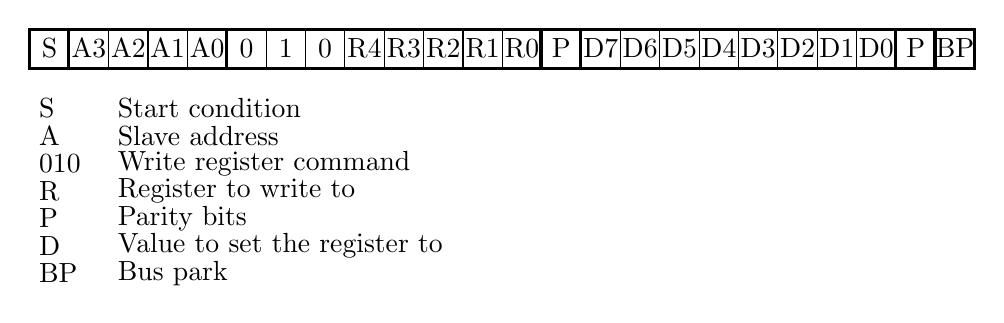
\begin{tikzpicture}[scale=0.5]
        \tikzstyle{bit} = [minimum height=5mm, minimum width=5mm, inner sep=0pt, draw];
        \foreach \i/\j in {
            0/S, 
            1/A3, 2/A2, 3/A1, 4/A0,
            5/0, 6/1, 7/0, 8/R4, 9/R3, 10/R2, 11/R1, 12/R0, 13/P,
            14/D7, 15/D6, 16/D5, 17/D4, 18/D3, 19/D2, 20/D1, 21/D0, 22/P,
            23/BP
        } {
            \node [bit,anchor=south west] at (\i,0) {\j};
        };

        \draw[very thick] (0,0) rectangle (1,1);
        \draw[very thick] (1,0) rectangle (5,1);
        \draw[very thick] (5,0) rectangle (13,1);
        \draw[very thick] (13,0) rectangle (14,1);
        \draw[very thick] (14,0) rectangle (22,1);
        \draw[very thick] (22,0) rectangle (23,1);
        \draw[very thick] (23,0) rectangle (24,1);

        \tikzstyle{T} = [anchor=west];
        \begin{scope}[yshift=-10mm, yscale=0.7]
            \foreach \i/\j/\l in {
                0/S/Start condition,
                1/A/Slave address,
                2/010/Write register command,
                3/R/Register to write to,
                4/P/Parity bits,
                5/D/Value to set the register to,
                6/BP/Bus park
            } {
                \node[T] at (0,-\i) {\j};
                \node[T] at (2,-\i) {\l};
            };
        \end{scope}
    \end{tikzpicture}
    \caption{RFFE command for writing to a register.}
    \label{fig:rffe_write_register}
\end{figure}
The RFFE command used for writing to a register is shown in Figure~\ref{fig:rffe_write_register}. The sequence is clocked out serially. A one bit is observed when the SCLK line goes high while the SDATA line is high and a zero bit is observed when the SCLK line goes high while the SDATA line is low. The start, parity, and bus park condition are described as follows:
\begin{description}
    \item[Start] SDATA pulses high while the SCLK line is kept low.
    \item[Parity] The parity is low if the number of ones in the preceding byte is odd. The parity is high if the number of ones in the preceding byte is even.
    \item[Bus park] SCLK is pulsed while SDATA is kept low (i.e.\ a zero is clocked out).
\end{description}
An example of and RFFE Write Register command is shown in Figure~\ref{fig:rffe_example}, where \texttt{0x00} is written to register 1 of the slave with address \texttt{0b0111}. This is the RFFE output when sending the string \texttt{"Ax0"} to the microcontroller, according to Table~\ref{tab:rffe_commands}.

\begin{figure}[htbp]
    \centering
    \includegraphics{img/optical_rffe/avr_rffe_reg1_0x00}
    \caption{Example of an RFFE command from the microcontroller.}
    \label{fig:rffe_example}
\end{figure}

\section{Level Shifting and WS1040 Interface}
The final part of the circuit is the interface towards the tuner. The microcontroller outputs signals between \SI{0}{V} and \SI{3.3}{V} which is not compatible with the tuner. Therefore, a level shifter is inserted, translating the \SI{3.3}{V} to \SI{1.8}{V}. The \SI{1.8}{V} is generated by a low-dropout voltage regulator.

% \section{User Effect - Simulation}


\subsubsection{Hand Simulation}
\begin{itemize}
\item 1 hand - Data mode
\begin{itemize}
\item Align antenna design with upper spacer.
\item Move the antenna design down until touching the lower spacer
\item If the antenna is longer than the lenght from the lower to the upper spacer, the antenna design exceeds the upper spacer.
\end{itemize}
\item 2 hand - read mode
\begin{itemize}
\item No standards for this mode - The Antenna design is placed as wanted.  
\end{itemize}
\end{itemize}

\subsubsection{Head Simulation}
\begin{itemize}
\item SAR measurement
\item Antenna design is aligned with the Antenna design in the ``1-simpler3 sar.cst'' phantom CST file. In the CST file, the antenna design is aligned, so that it barely touches the cheek, whereas in the ``SAR without hand.cst'' file only can be used for the bodyloss of head and hand.
\end{itemize}


% Back matter %%%%%%%%%%%%%%%%%%%%%%%%%%%%%%%%%%%%%%%%%%%%%%%%%%%%%%%%%%%%%%%%%%

\listoffixmes
\bibliographystyle{ieeetr}
\bibliography{bib/sources}
\addcontentsline{toc}{chapter}{Bibliography}

\end{document}
